% ------------------------------------------------------------------------------
% Chapter 2
% ------------------------------------------------------------------------------
\chapter{Summary of the Approach to EDA and Pre-processing}
\label{cha:chapter 2}

In this chapter, we perform an exploratory data analysis (EDA) to gain a deeper understanding of the dataset and uncover insights that will guide the development of our pneumonia detection algorithm. EDA is a critical step in the data science process, as it helps to identify patterns, detect anomalies, and test hypotheses. By visualizing and summarizing the dataset, we can better understand its structure, identify potential issues, and make informed decisions about data preprocessing and model selection.

\section{Exploratory Data Analysis (EDA)}
\label{sec:chap2 section 1}

\subsection{Overview of the Dataset:}
\label{subsec:chap2 section 1.1}

The dataset contained two CSV files: one with class labels and patient IDs and another with bounding box coordinates. The boudning box data has the format given in Table~\ref{tab:cha-2 table1}.

\begin{table}[h!]
    \centering
    \caption{Training Boudning Box Data}
    \label{tab:cha-2 table1}
    \begin{tabular}{c|c|c|c|c|c|c}
        \rowcolor{gray!20}
        \textbf{Index} & \textbf{patientId}                   & \textbf{x} & \textbf{y} & \textbf{width} & \textbf{height} & \textbf{Target} \\
        0              & 0004cfab-14fd-4e49-80ba-63a80b6bddd6 & NaN        & NaN        & NaN            & NaN             & 0               \\
        1              & 00313ee0-9eaa-42f4-b0ab-c148ed3241cd & NaN        & NaN        & NaN            & NaN             & 0               \\
        2              & 00322d4d-1c29-4943-afc9-b6754be640eb & NaN        & NaN        & NaN            & NaN             & 0               \\
        3              & 003df8a0-6bf1-40ed-b54c-ac657f8495c5 & NaN        & NaN        & NaN            & NaN             & 0               \\
        4              & 00436515-870c-4b36-a041-de91049b9ab4 & 264.0      & 152.0      & 213.0          & 379.0           & 1               \\
        5              & 00436515-870c-4b36-a041-de91049b9ab4 & 562.0      & 152.0      & 256.0          & 453.0           & 1               \\
    \end{tabular}
\end{table}

The file, which contains the bouding boxes coordinates, provides essential information about the bounding boxes and targets associated with each patient. This dataframe we created from the CSV file includes the following columns:

\begin{itemize}
    \item \textbf{patientId:} A unique identifier for each patient.
    \item \textbf{x:} The x-coordinate of the bounding box, indicating its horizontal position.
    \item \textbf{y:} The y-coordinate of the bounding box, indicating its vertical position.
    \item \textbf{width:} The width of the bounding box.
    \item \textbf{height:} The height of the bounding box.
    \item \textbf{Target:} A binary label indicating the presence of pneumonia (1) or its absence (0).
\end{itemize}

The dataset consists of 30,227 entries, with bounding box coordinates ($x$, $y$, width, height) provided for 9,555 entries where pneumonia is present (Target = 1). The remaining 20,722 entries, where Target = 0, have null values for the bounding box coordinates, indicating the absence of pneumonia.

The second file contains the training labels data, which has the format given in Table~\ref{tab:cha-2 table2}.

\begin{table}[h!]
    \centering
    \caption{Training Labels Data}
    \label{tab:cha-2 table2}
    \begin{tabular}{c|l|l}
        \rowcolor{gray!20}
        \textbf{Index} & \textbf{patientId}                   & \textbf{class}               \\
        0              & 0004cfab-14fd-4e49-80ba-63a80b6bddd6 & No Lung Opacity / Not Normal \\
        1              & 00313ee0-9eaa-42f4-b0ab-c148ed3241cd & No Lung Opacity / Not Normal \\
        2              & 00322d4d-1c29-4943-afc9-b6754be640eb & No Lung Opacity / Not Normal \\
        3              & 003df8a0-6bf1-40ed-b54c-ac657f8495c5 & Normal                       \\
        4              & 00436515-870c-4b36-a041-de91049b9ab4 & Lung Opacity                 \\
        5              & 00436515-870c-4b36-a041-de91049b9ab4 & Lung Opacity                 \\
    \end{tabular}
\end{table}


The training labels is smiliarly converted to a dataframe. The data consists of 30227 entries, with each entry corresponding to a unique entry in the bounding box data. The dataframe contains the following columns:

\begin{itemize}
    \item \textbf{patientId:} A unique identifier for each patient, which is consistent with the identifiers in the training label data.
    \item \textbf{class:} A categorical label indicating the status of the lung opacity in the chest radiographs. The possible values are:
          \begin{itemize}
              \item \textbf{No Lung Opacity / Not Normal:} Indicates that while pneumonia is not present, there is some abnormality in the image that may mimic the appearance of pneumonia.
                    \textbf{Lung Opacity:} Indicates the presence of pneumonia.
                    \textbf{Normal:} Indicates that there are no abnormalities or pneumonia present in the image.
          \end{itemize}
\end{itemize}

The key points to note from the training labels data are:
\begin{itemize}
    \item The dataframe includes 30,227 entries, with each entry corresponding to a unique patient ID.
    \item The class labels help in distinguishing between normal images, images with lung opacity (pneumonia), and images with other abnormalities.
    \item There are no missing values in either the patientId or class columns, ensuring a complete dataset for analysis.
\end{itemize}

The training and testing images are provided in two separate folders, with each image name corresponding to a unique patient ID. We created a dataframe that maps each patient ID to the corresponding image file path, which will be used to load and preprocess the images for model training. Table ~\ref{tab:cha-2 table3} shows the format of the dataframe containing the image file paths.

\begin{table}[h!]
    \centering
    \caption{Image File Paths Data}
    \label{tab:cha-2 table3}
    \begin{adjustbox}{max width=\textwidth}
        \begin{tabularx}{\textwidth}{c|X|X}
            \rowcolor{gray!20}
            \textbf{Index} & \textbf{path}                    & \textbf{patientId} \\
            0              & data/..train\_images/ec811ac3-.. & ec811ac3-..        \\
            1              & data/..train\_images/a45992b1-.. & a45992b1-..        \\
            2              & data/..train\_images/b1d07564-.. & b1d07564-..        \\
            3              & data/..train\_images/a0c6c07c-.. & a0c6c07c-..        \\
        \end{tabularx}
    \end{adjustbox}
\end{table}

There are 26684 images in the training dataset and 3000 images in the test dataset. The number of training images match with the number of unique patient IDs in the training labels data, indicating that each patient has an associated image.

\textbf{Bounding Box Consistency:} We confirmed that the number of bounding boxes for a patient in the bouding box dataframe matches the number of entries for that patient in the class label dataframe. This consistency indicates that the bounding box annotations are correctly aligned with the class labels.

\textbf{Unique Classes per Patient:} Each patient ID is associated with only one class, ensuring that there are no conflicting class labels for a single patient. This was verified by grouping the class label dataframe by $patientId$ and checking the number of unique classes for each patient.

Further, we inspected the metadata associated with the medical images. This metadata provides valuable information about the image acquisition process, patient details, and other relevant attributes. By extracting and analyzing this metadata, we can gain deeper insights into the dataset and ensure the consistency and quality of the data used for model training.

\textbf{Reading a Sample Image File:}
\begin{itemize}
    \item A sample DICOM image file was read to inspect its metadata. The metadata includes a variety of fields such as the modality, patient ID, patient age, view position, and more.
    \item Relevant metadata fields were extracted from the DICOM files and stored in a dataframe for further analysis. Table ~\ref{tab:cha-2 table4} shows the format of the dataframe containing the extracted metadata fields.
    \item The extracted fields include \emph{path, patientId, patientSex, patientAge,} and \emph{viewPosition}

\end{itemize}

\begin{table}[h!]
    \centering
    \caption{Metadata from DICOM Images}
    \label{tab:cha-2 table4}
    \begin{adjustbox}{max width=\textwidth}
        \begin{tabularx}{\textwidth}{c|X|X|c|c|c|c}
            \rowcolor{gray!20}
            \textbf{Index} & \textbf{path}    & \textbf{patientId} & \textbf{patientSex} & \textbf{patientAge} & \textbf{viewPosition} \\
            0              & data/..images/.. & ec811ac3-..        & M                   & 51.0                & AP                    \\
            1              & data/..images/.. & a45992b1-..        & M                   & 24.0                & PA                    \\
            2              & data/..images/.. & b1d07564-..        & M                   & 51.0                & AP                    \\
        \end{tabularx}
    \end{adjustbox}
\end{table}

\subsection{Distribution and skewness of Classes and Variables:}
\label{subsec:chap2 section 1.2}

Understanding the distribution of classes in the dataset is crucial for developing a robust deep learning model. The class distribution helps in identifying any imbalances that may exist, which can impact model training and performance. We first analysed the Targets in the training labels data to determine the distribution of pneumonia cases in the dataset. This is done after removing outliers, which is discussed in section~\ref{subsec:chap2 section 1.6}.

\begin{figure}[H]
    \begin{center}
        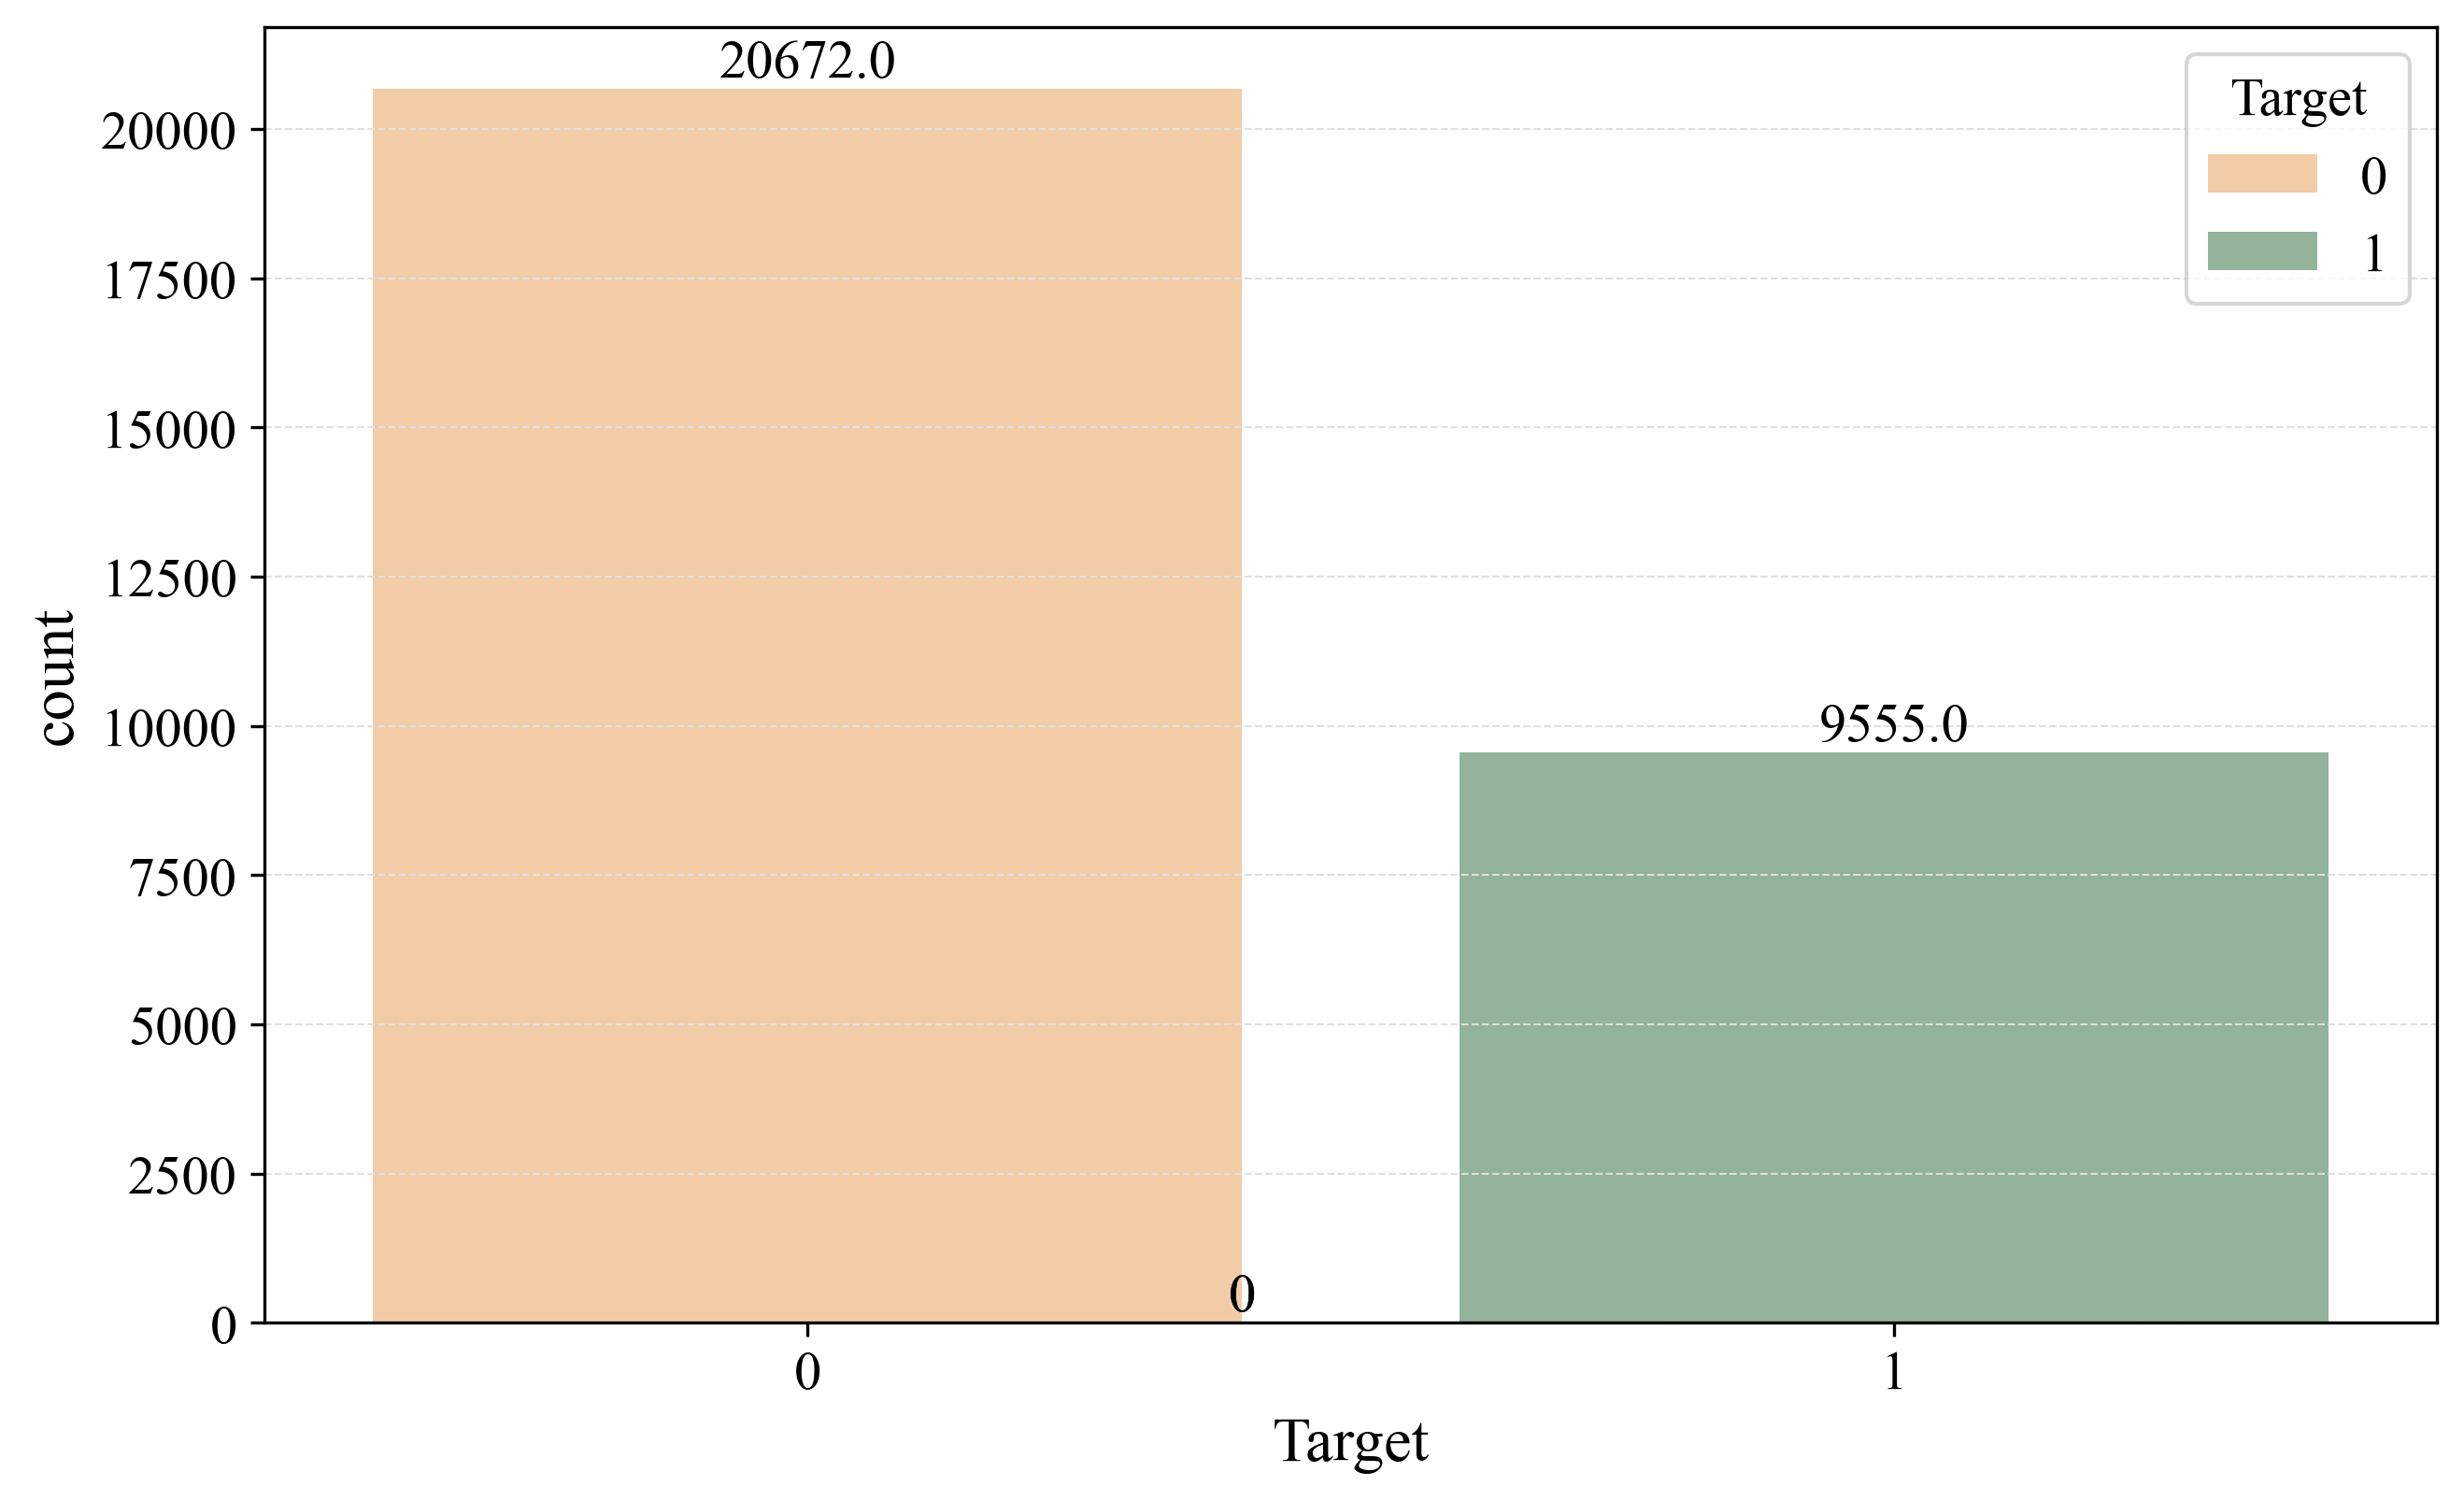
\includegraphics[width = 0.6\textwidth]{figures/Figure1.png}
        \caption{The count of $Target$ column in the training data}
        \label{fig:cha-2 figure1}
    \end{center}
\end{figure}

\textbf{Main Points:}

\begin{itemize}
    \item For patients with no pneumonia, the bounding box coordinates ($x$, $y$, width, height) are null.
    \item There are a total of 20,672 rows with null bouding box coordinates, indicating the absence of pneumonia.
    \item The correspoindg $Target$ value for these rows is 0.
    \item There are a total of 9,555 rows with non-null bounding box coordinates, indicating the presence of pneumonia.
    \item The corresponding $Target$ value for these rows is 1.
\end{itemize}

The distribution of the $Target$ variable is visualized in Figure~\ref{fig:cha-2 figure1}. The plot shows a significant class imbalance, with a higher number of cases labeled as $Target = 0$ (no pneumonia) compared to $Target = 1$ (pneumonia present). This imbalance can potentially affect the performance of the model, as it may become biased towards predicting the majority class (no pneumonia) while training for predicting the $Target$.
To address this imbalance, techniques such as resampling (oversampling the minority class or undersampling the majority class), using class weights, or applying data augmentation can be employed.

Next we analyzed the $class$ column in the training labels data to understand the distribution of class labels in the dataset. The distribution of classes is visualized in Figure~\ref{fig:cha-2 figure2}.


\begin{figure}[H]
    \begin{center}
        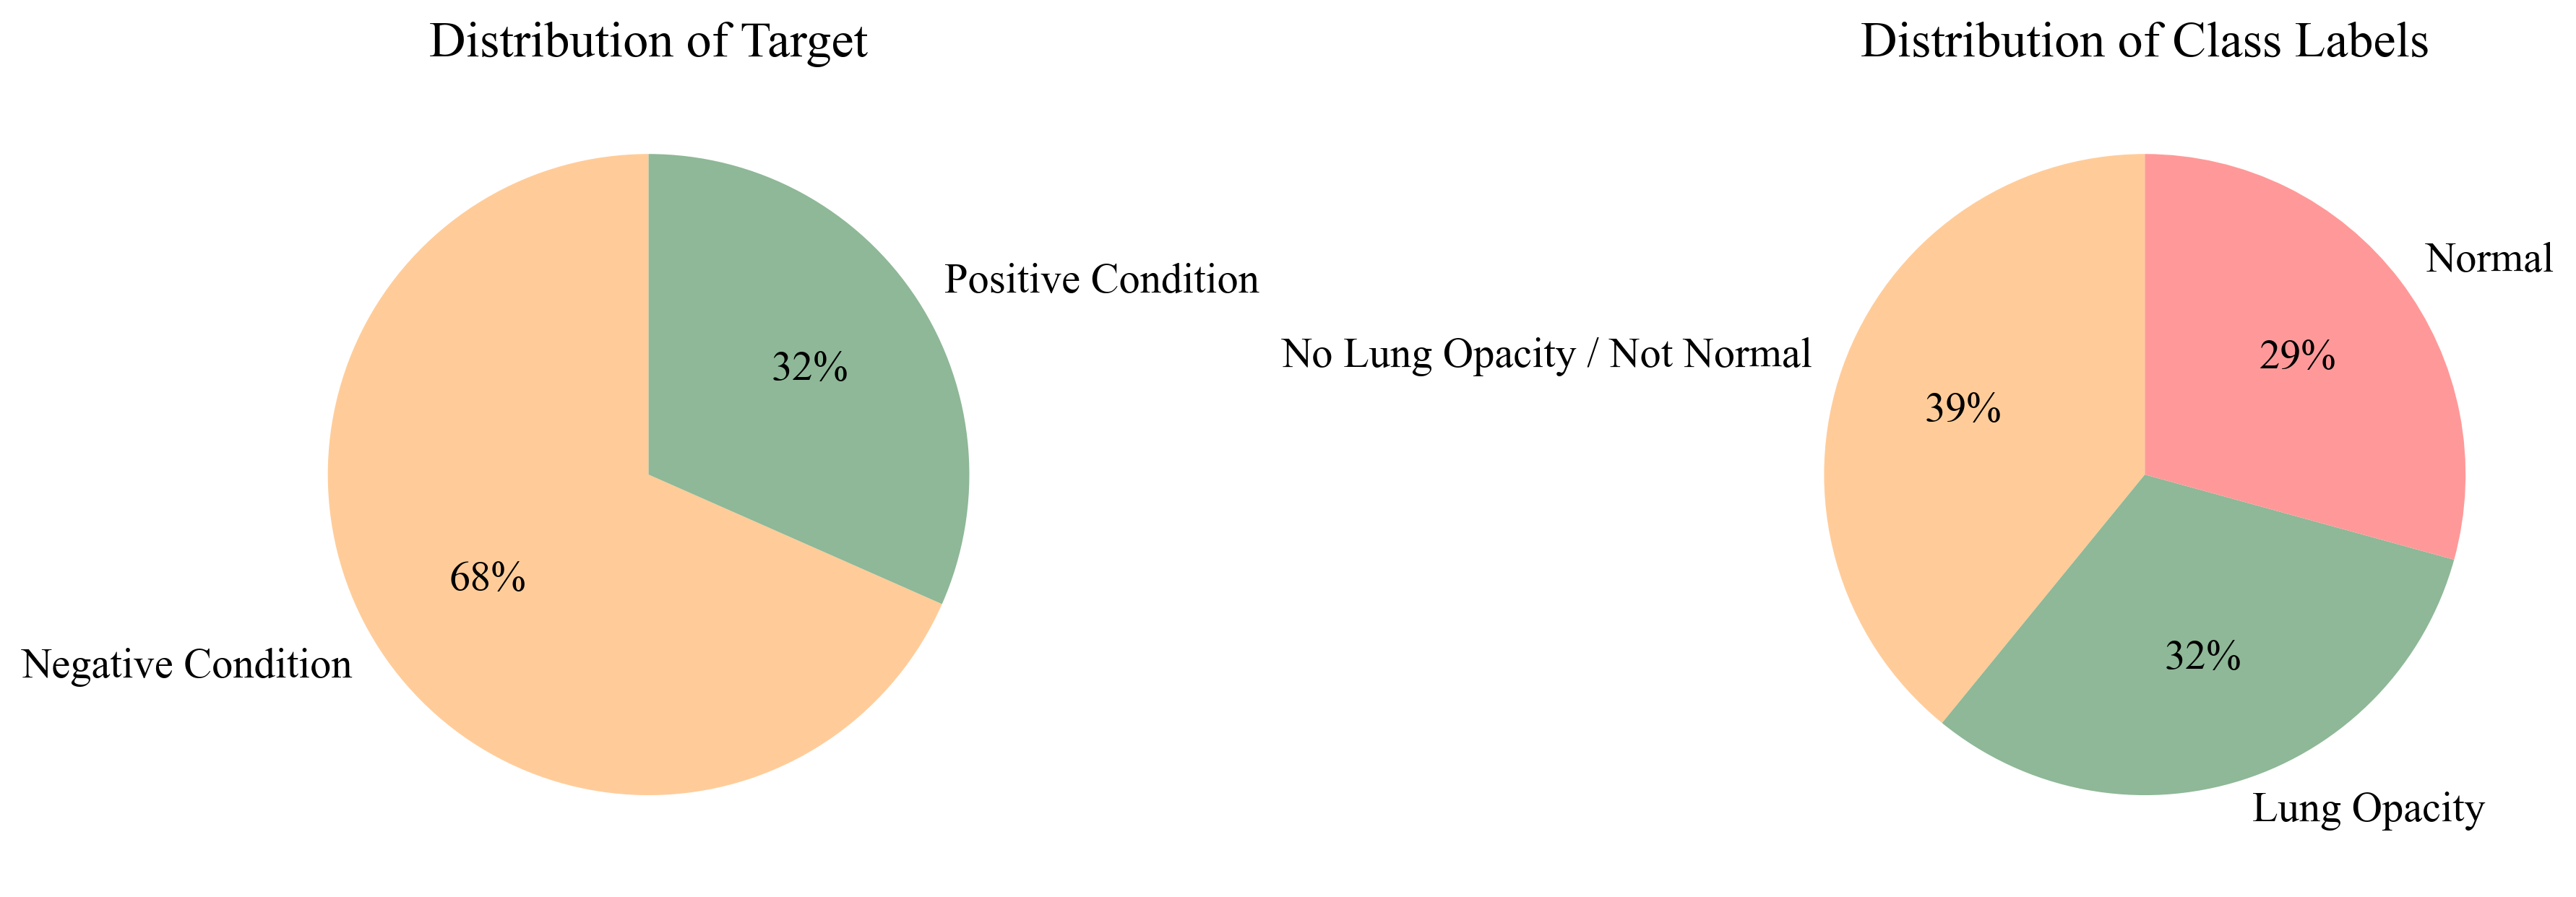
\includegraphics[width = 1.0\textwidth]{figures/Figure4.png}
        \caption{The distribution of $class$ labels in the training data compared to the $Target$ variable}
        \label{fig:cha-2 figure2}
    \end{center}
\end{figure}

Although the overall condition distribution is skewed towards the negative condition, the negative condition itself comprises two sub-classes, which helps in moderating the imbalance. The \emph{No Lung Opacity / Not Normal class} has the highest proportion of records (39\%), followed by the \emph{Lung Opacity} class (32\%), and the \emph{Normal} class (29\%).

The histograms in Figure ~\ref{fig:cha-2 figure3} and Figure ~\ref{fig:cha-2 figure4} show the distribution of the $patientAge$ within each class binned with different intervals for better understanding.

\begin{figure}[H]
    \begin{center}
        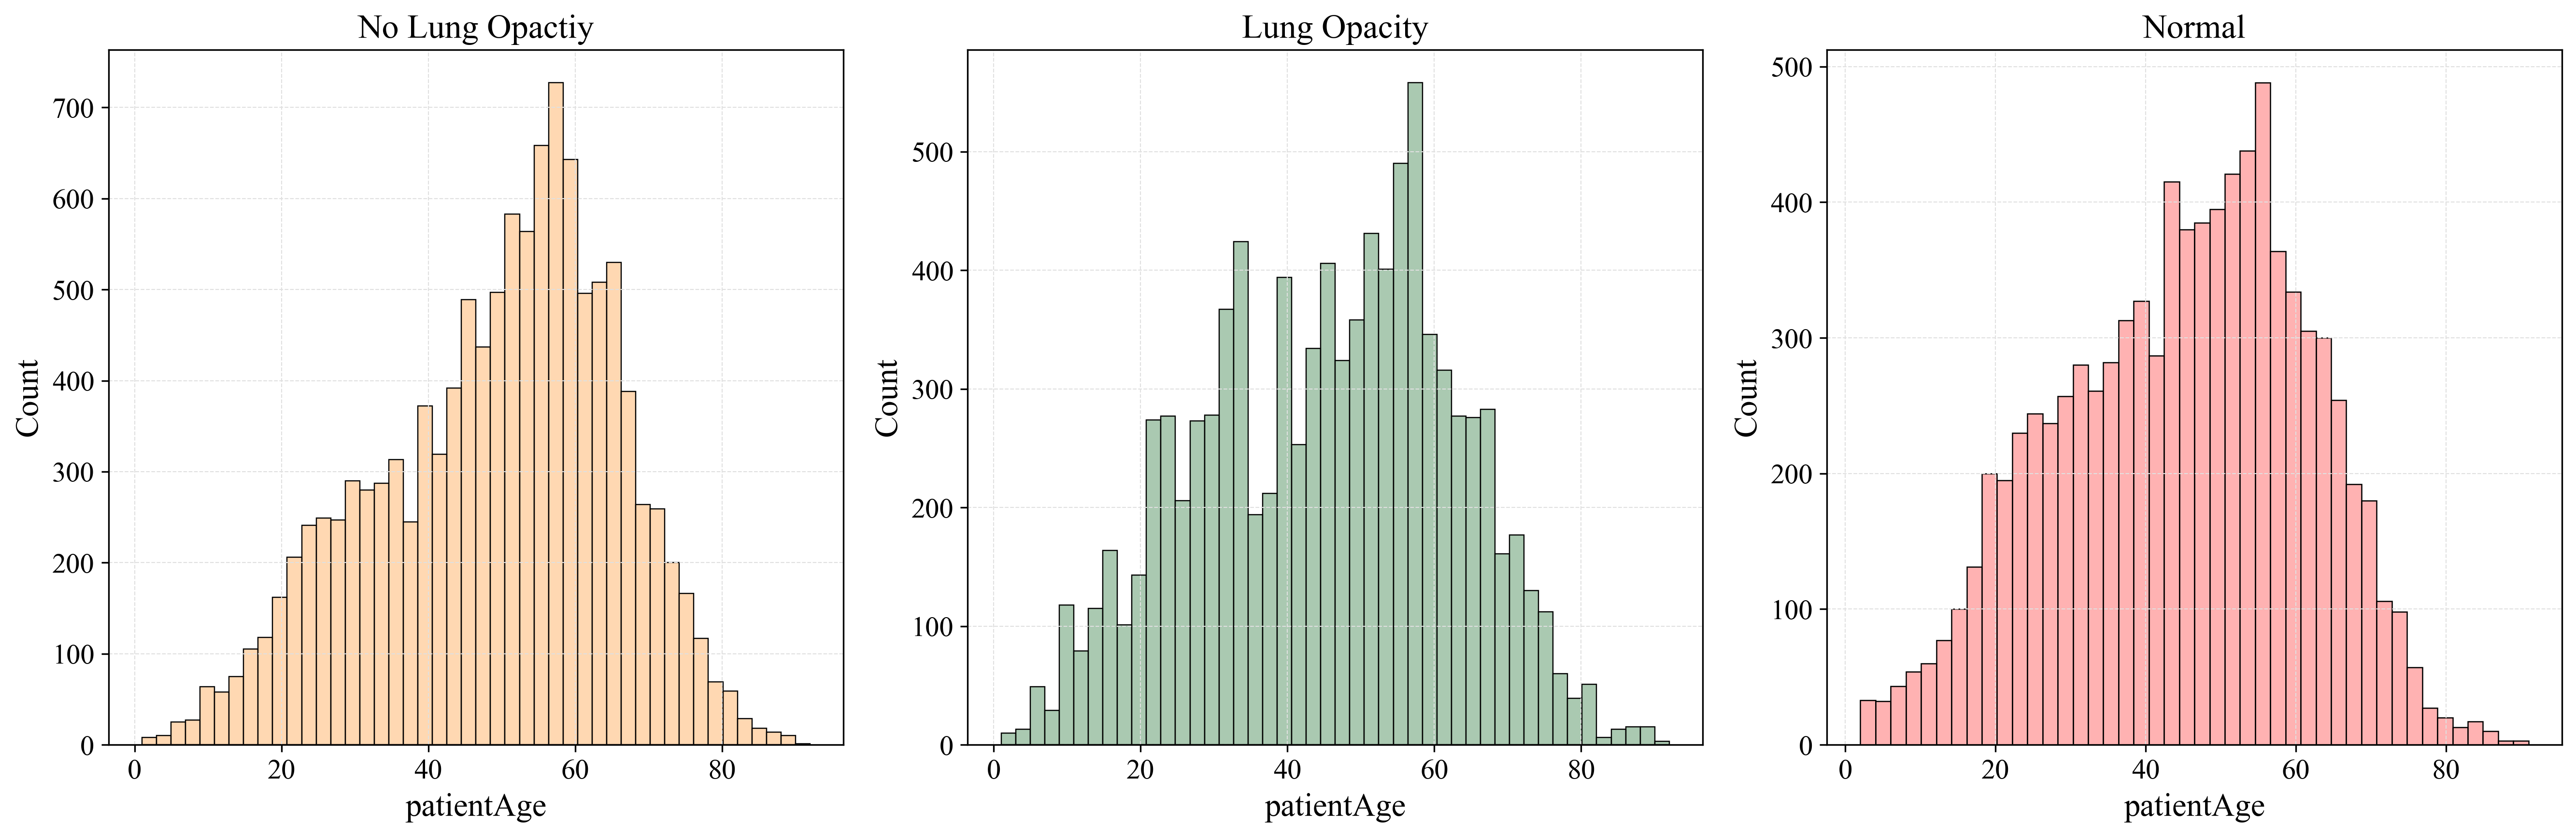
\includegraphics[width = 1.0\textwidth]{figures/Figure5.png}
        \caption{Distribution of $patientAge$ within each class binned at an interval of 2 years}
        \label{fig:cha-2 figure3}
    \end{center}
\end{figure}

\begin{figure}[H]
    \begin{center}
        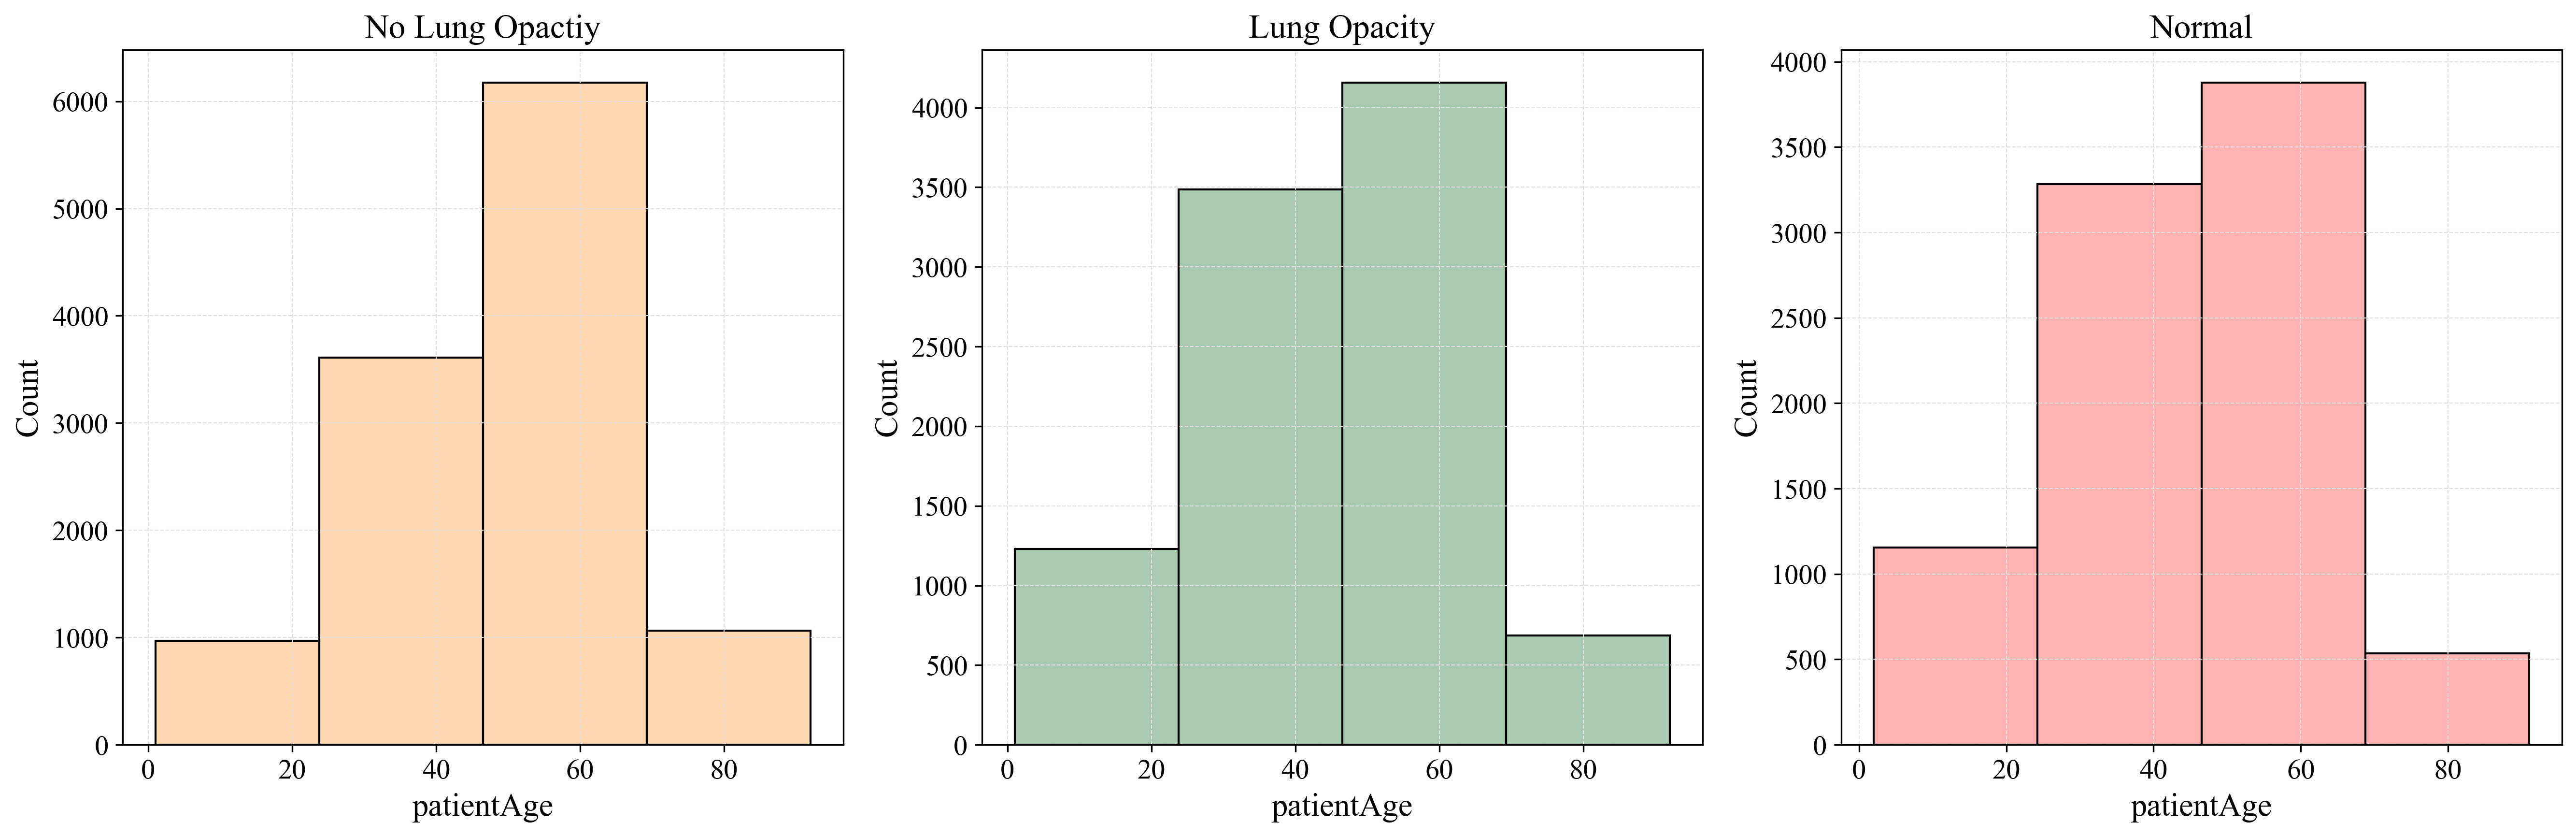
\includegraphics[width = 1.0\textwidth]{figures/Figure6.png}
        \caption{Distribution of $patientAge$ within each class binned at an interval of 25 years}
        \label{fig:cha-2 figure4}
    \end{center}
\end{figure}

\textbf{No Lung Opacity / Not Normal:}
\begin{itemize}
    \item The age distribution for this class shows a peak around 60 years, with a relatively balanced distribution around this peak.
    \item This class contains a significant number of middle-aged and elderly patients.
\end{itemize}

\textbf{Lung Opacity (Pneumonia):}
\begin{itemize}
    \item The age distribution for the pneumonia class also peaks around 60 years but shows a more balanced spread across different age groups.
    \item There is a noticeable presence of pneumonia cases in both younger and older patients.
\end{itemize}

\textbf{Normal:}
\begin{itemize}
    \item The age distribution for the normal class peaks around 55 years, with a relatively balanced distribution around this peak.
    \item This class also contains a significant number of middle-aged and elderly patients.
\end{itemize}

There is a noticeable skew towards middle-aged and elderly patients across all class labels. This skewness could be due to the higher likelihood of pneumonia and other lung conditions in older populations.
The presence of younger patients is relatively lower across all classes, which may impact the model's ability to generalize across different age groups. Despite the skew towards older age groups, the distribution within each class appears relatively balanced.

\subsection{Patient Demographics and Data Diversity}
\label{subsec:chap2 section 1.3}

To gain a comprehensive understanding of the dataset, it is important to analyze patient demographics, such as age and gender, across different class labels. This analysis provides insights into the representation of different patient groups within the dataset and helps in identifying any potential biases. For this we will plot the distribution of $patientSex$ and $patientAge$ across different class labels.

We have already observed in the previous section that the distribution of $patientAge$ appears roughly normal (bell-shaped) for all three class labels:\emph{No Lung Opacity / Not Normal},\emph{Lung Opacity}, and \emph{Normal}. The combined distrubtion of age across the three classes is shown in Figure~\ref{fig:cha-2 figure5}.

\begin{figure}[H]
    \begin{center}
        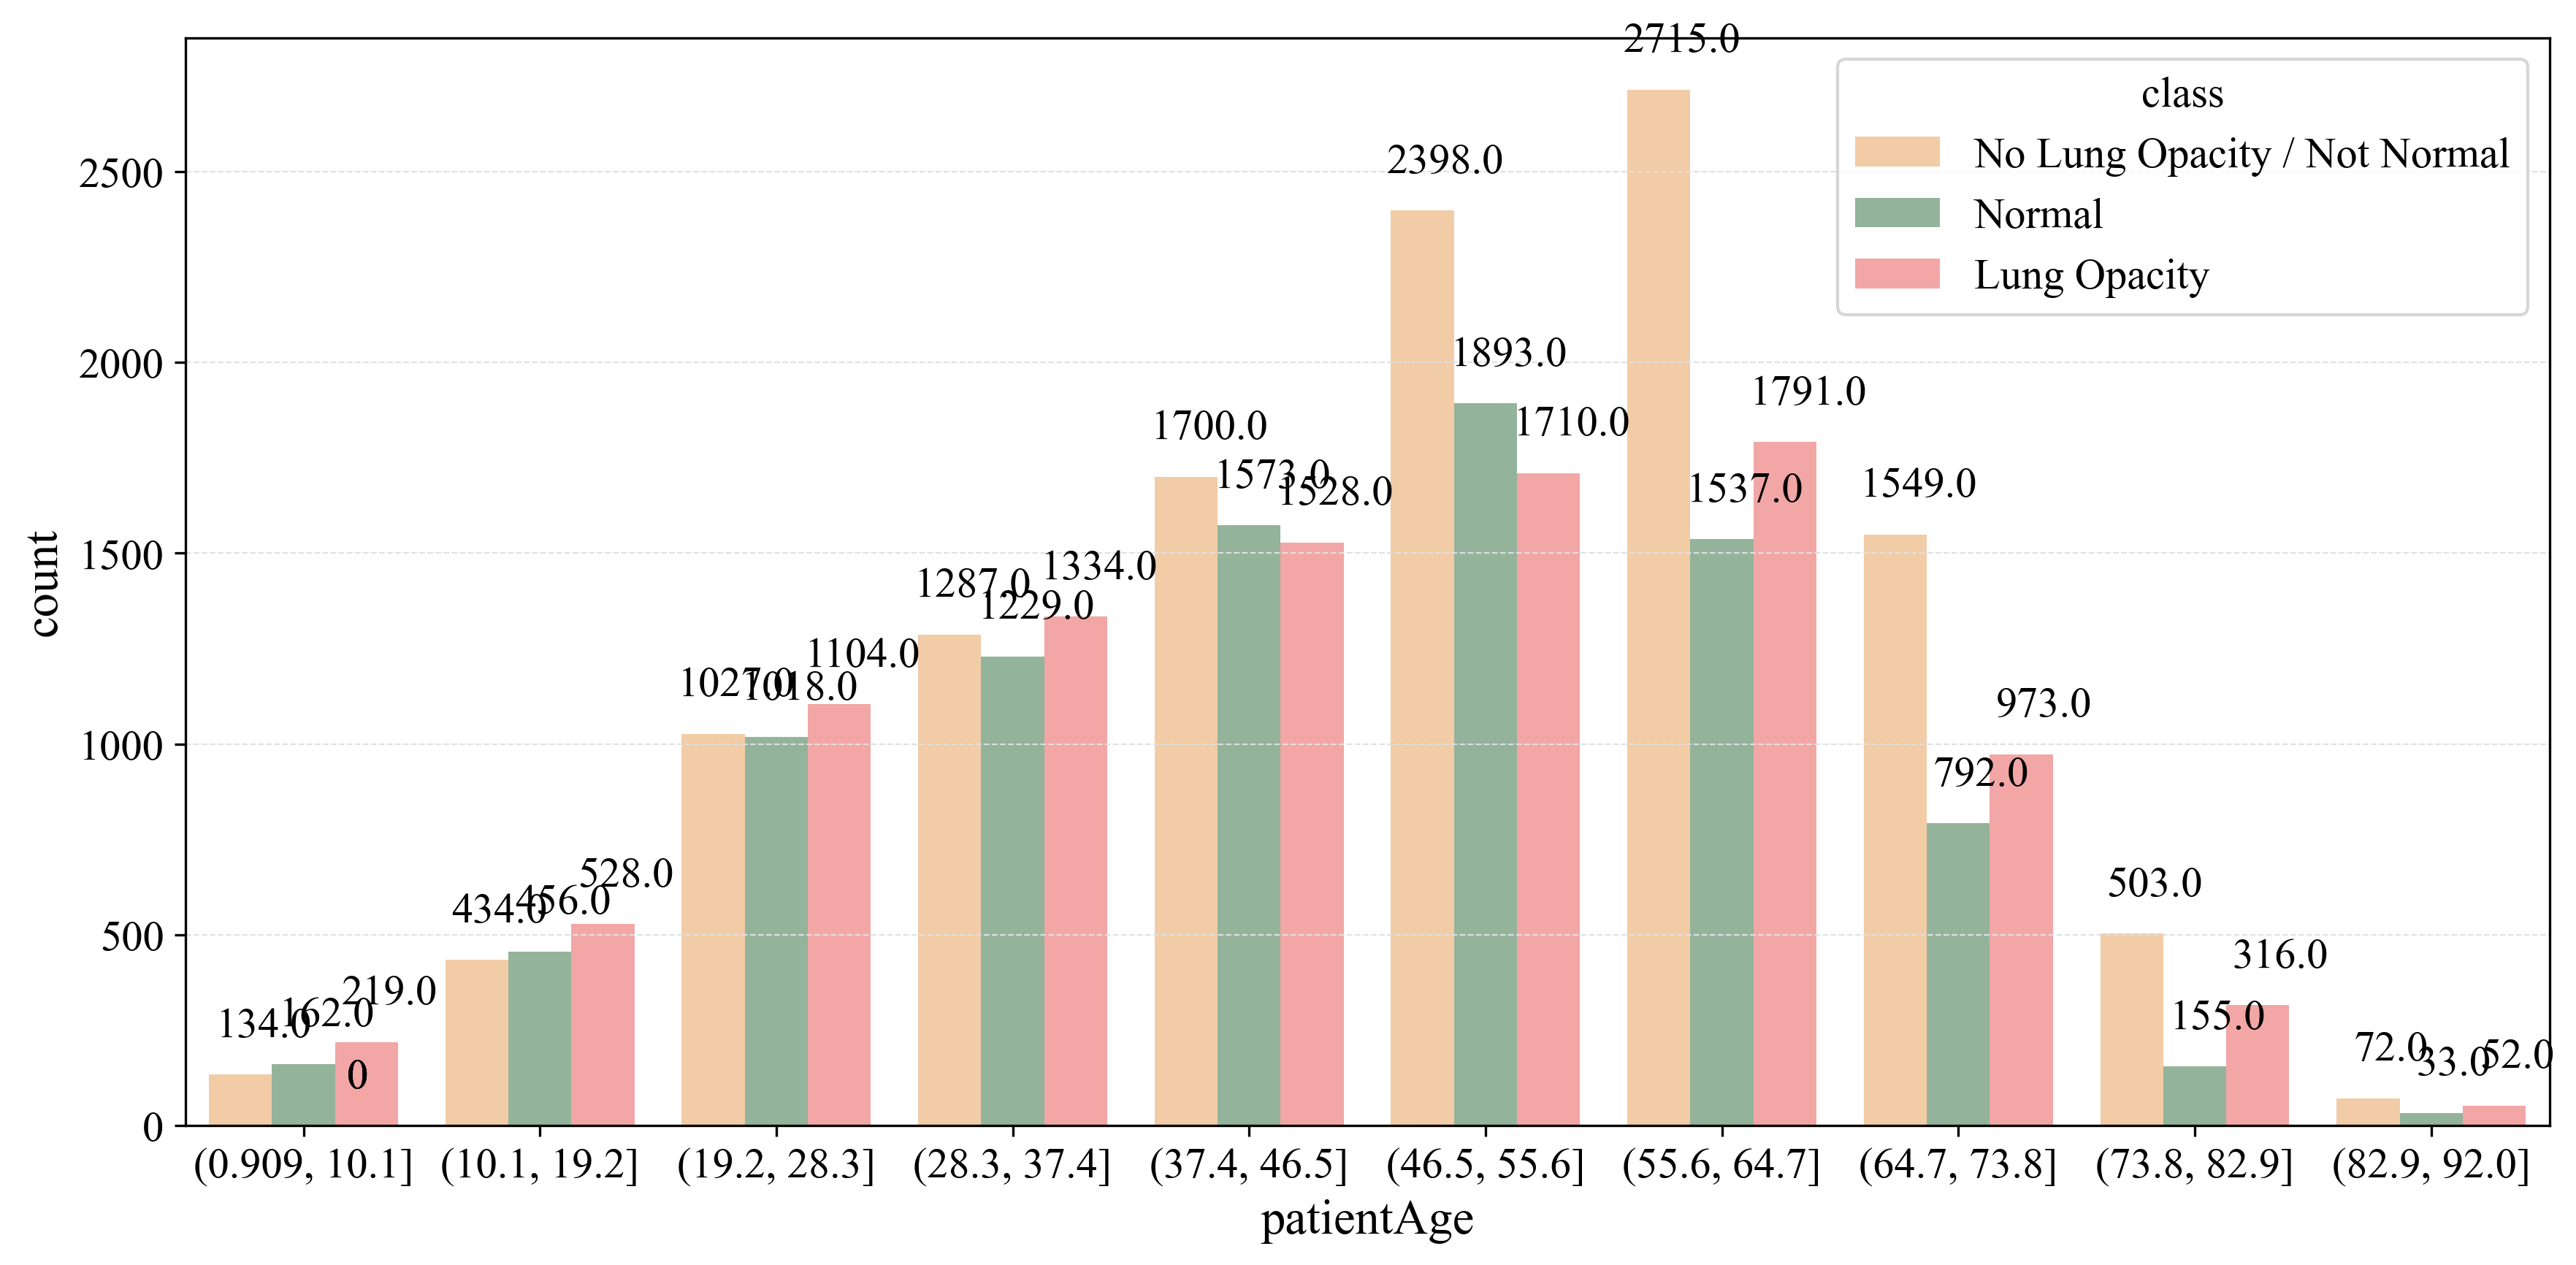
\includegraphics[width = 0.6\textwidth]{figures/Figure8.png}
        \caption{Distribution of $patientAge$ across all class labels}
        \label{fig:cha-2 figure5}
    \end{center}
\end{figure}

Figure~\ref{fig:cha-2 figure5} verifies that the peak age range is around 50 to 60 years for all distributions, indicating that this age group is most represented in the dataset. The similarity in age distribution across all three classes suggests that age cannot be a strong predictor of the class label.

There is a noticeable difference in the number of male and female patients across different classes. This is illustrated in Figure~\ref{fig:cha-2 figure6} and Figure~\ref{fig:cha-2 figure7} The number of male patients suffering from pneumonia (Lung Opacity) is greater compared to female patients. In the \emph{No Lung Opacity / Not Normal} class, and the \emph{Normal} classes,  the number of male patients is also higher than that of female patients.

\begin{figure}[H]
    \begin{center}
        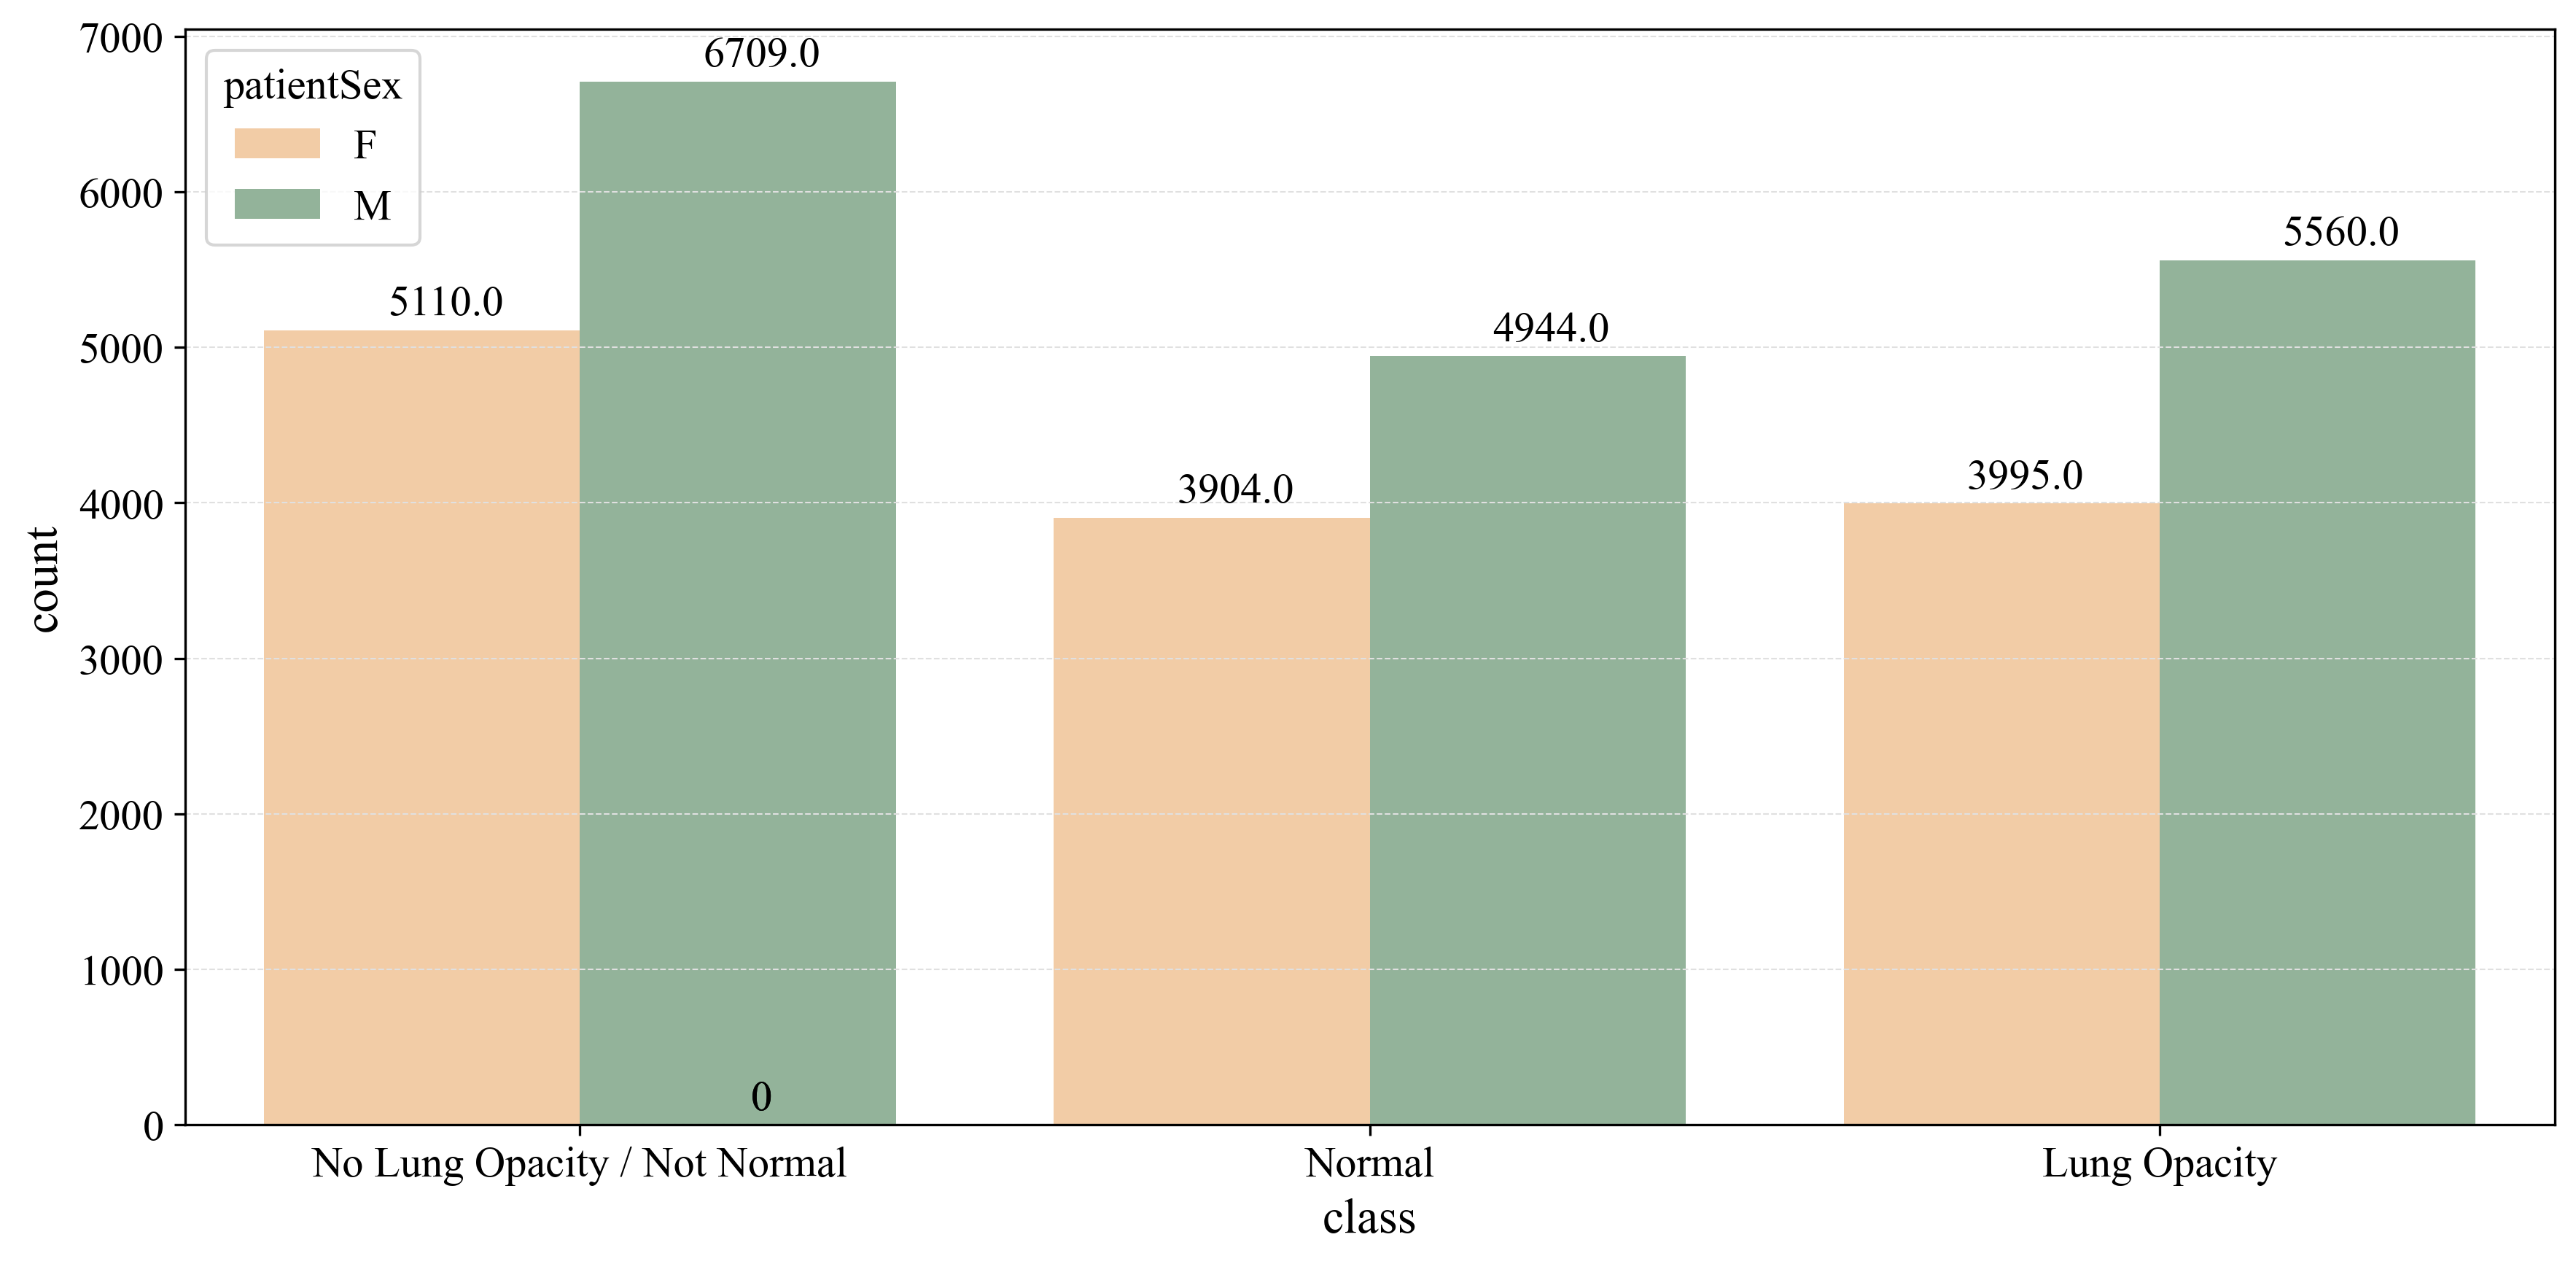
\includegraphics[width = 0.6\textwidth]{figures/Figure11.png}
        \caption{Distribution of $patientSex$ across all class labels}
        \label{fig:cha-2 figure6}
    \end{center}
\end{figure}

\begin{figure}[H]
    \begin{center}
        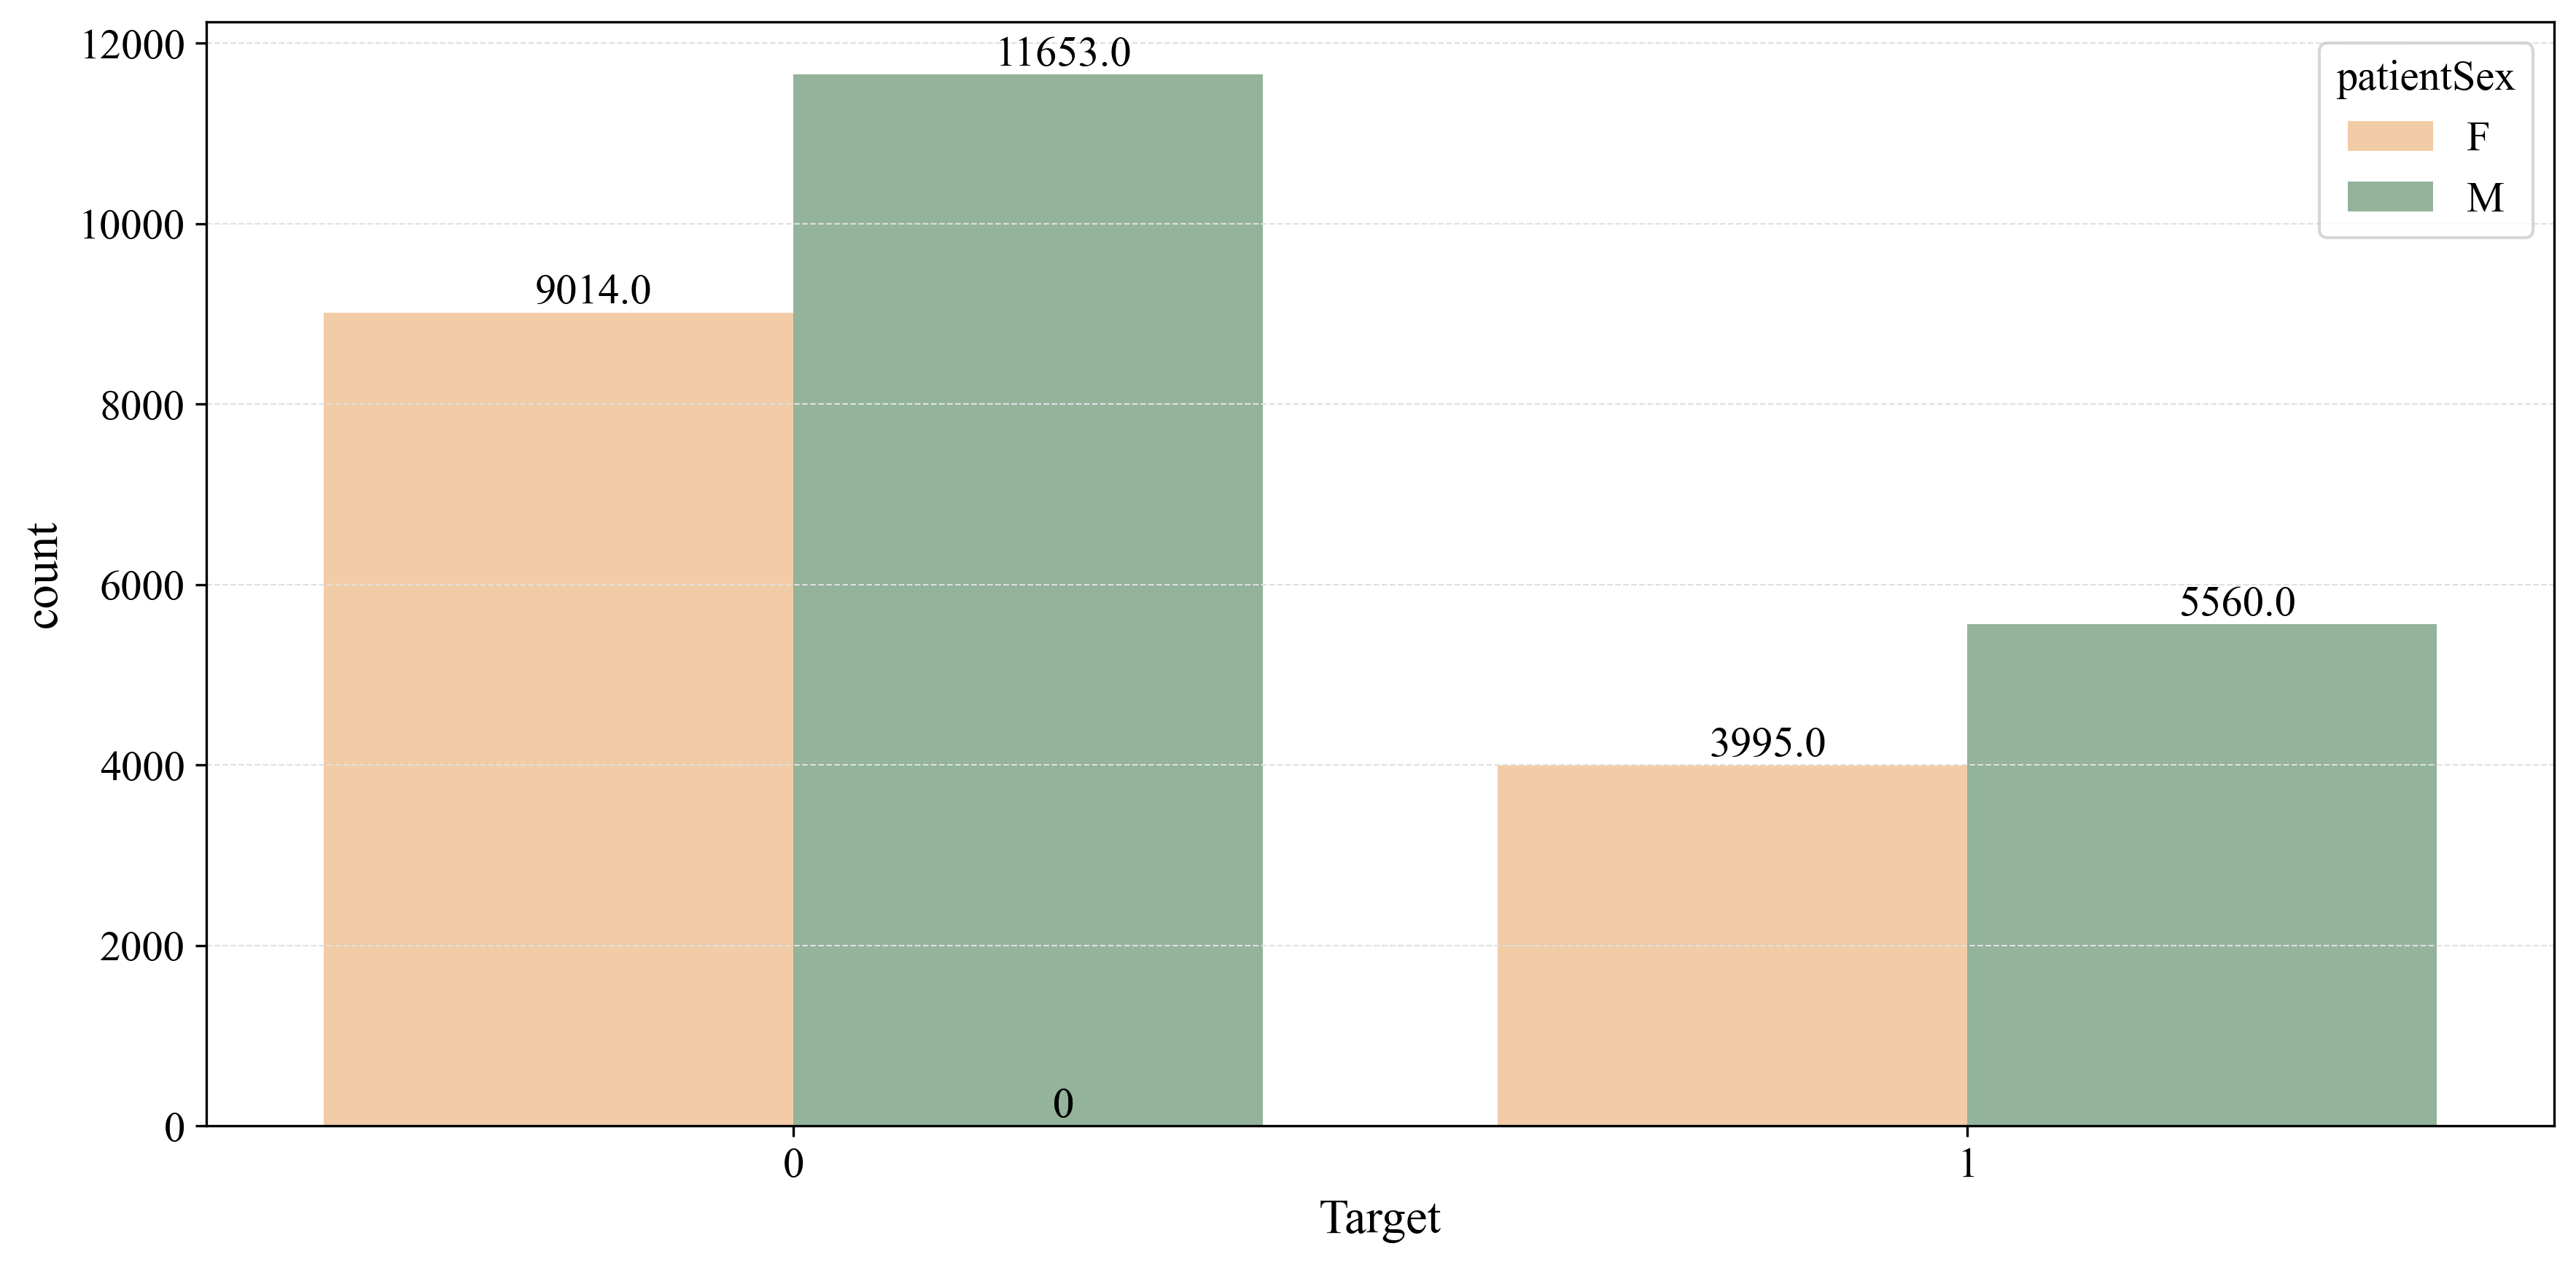
\includegraphics[width = 0.6\textwidth]{figures/Figure12.png}
        \caption{Distribution of $patientSex$ across Target}
        \label{fig:cha-2 figure7}
    \end{center}
\end{figure}

The dataset includes two view positions: Posterior-Anterior (PA) and Anterior-Posterior (AP). The distribution of view positions shows a relatively balanced representation of PA and AP views across different age groups as shown in Figure~\ref{fig:cha-2 figure8}.

\begin{figure}[H]
    \begin{center}
        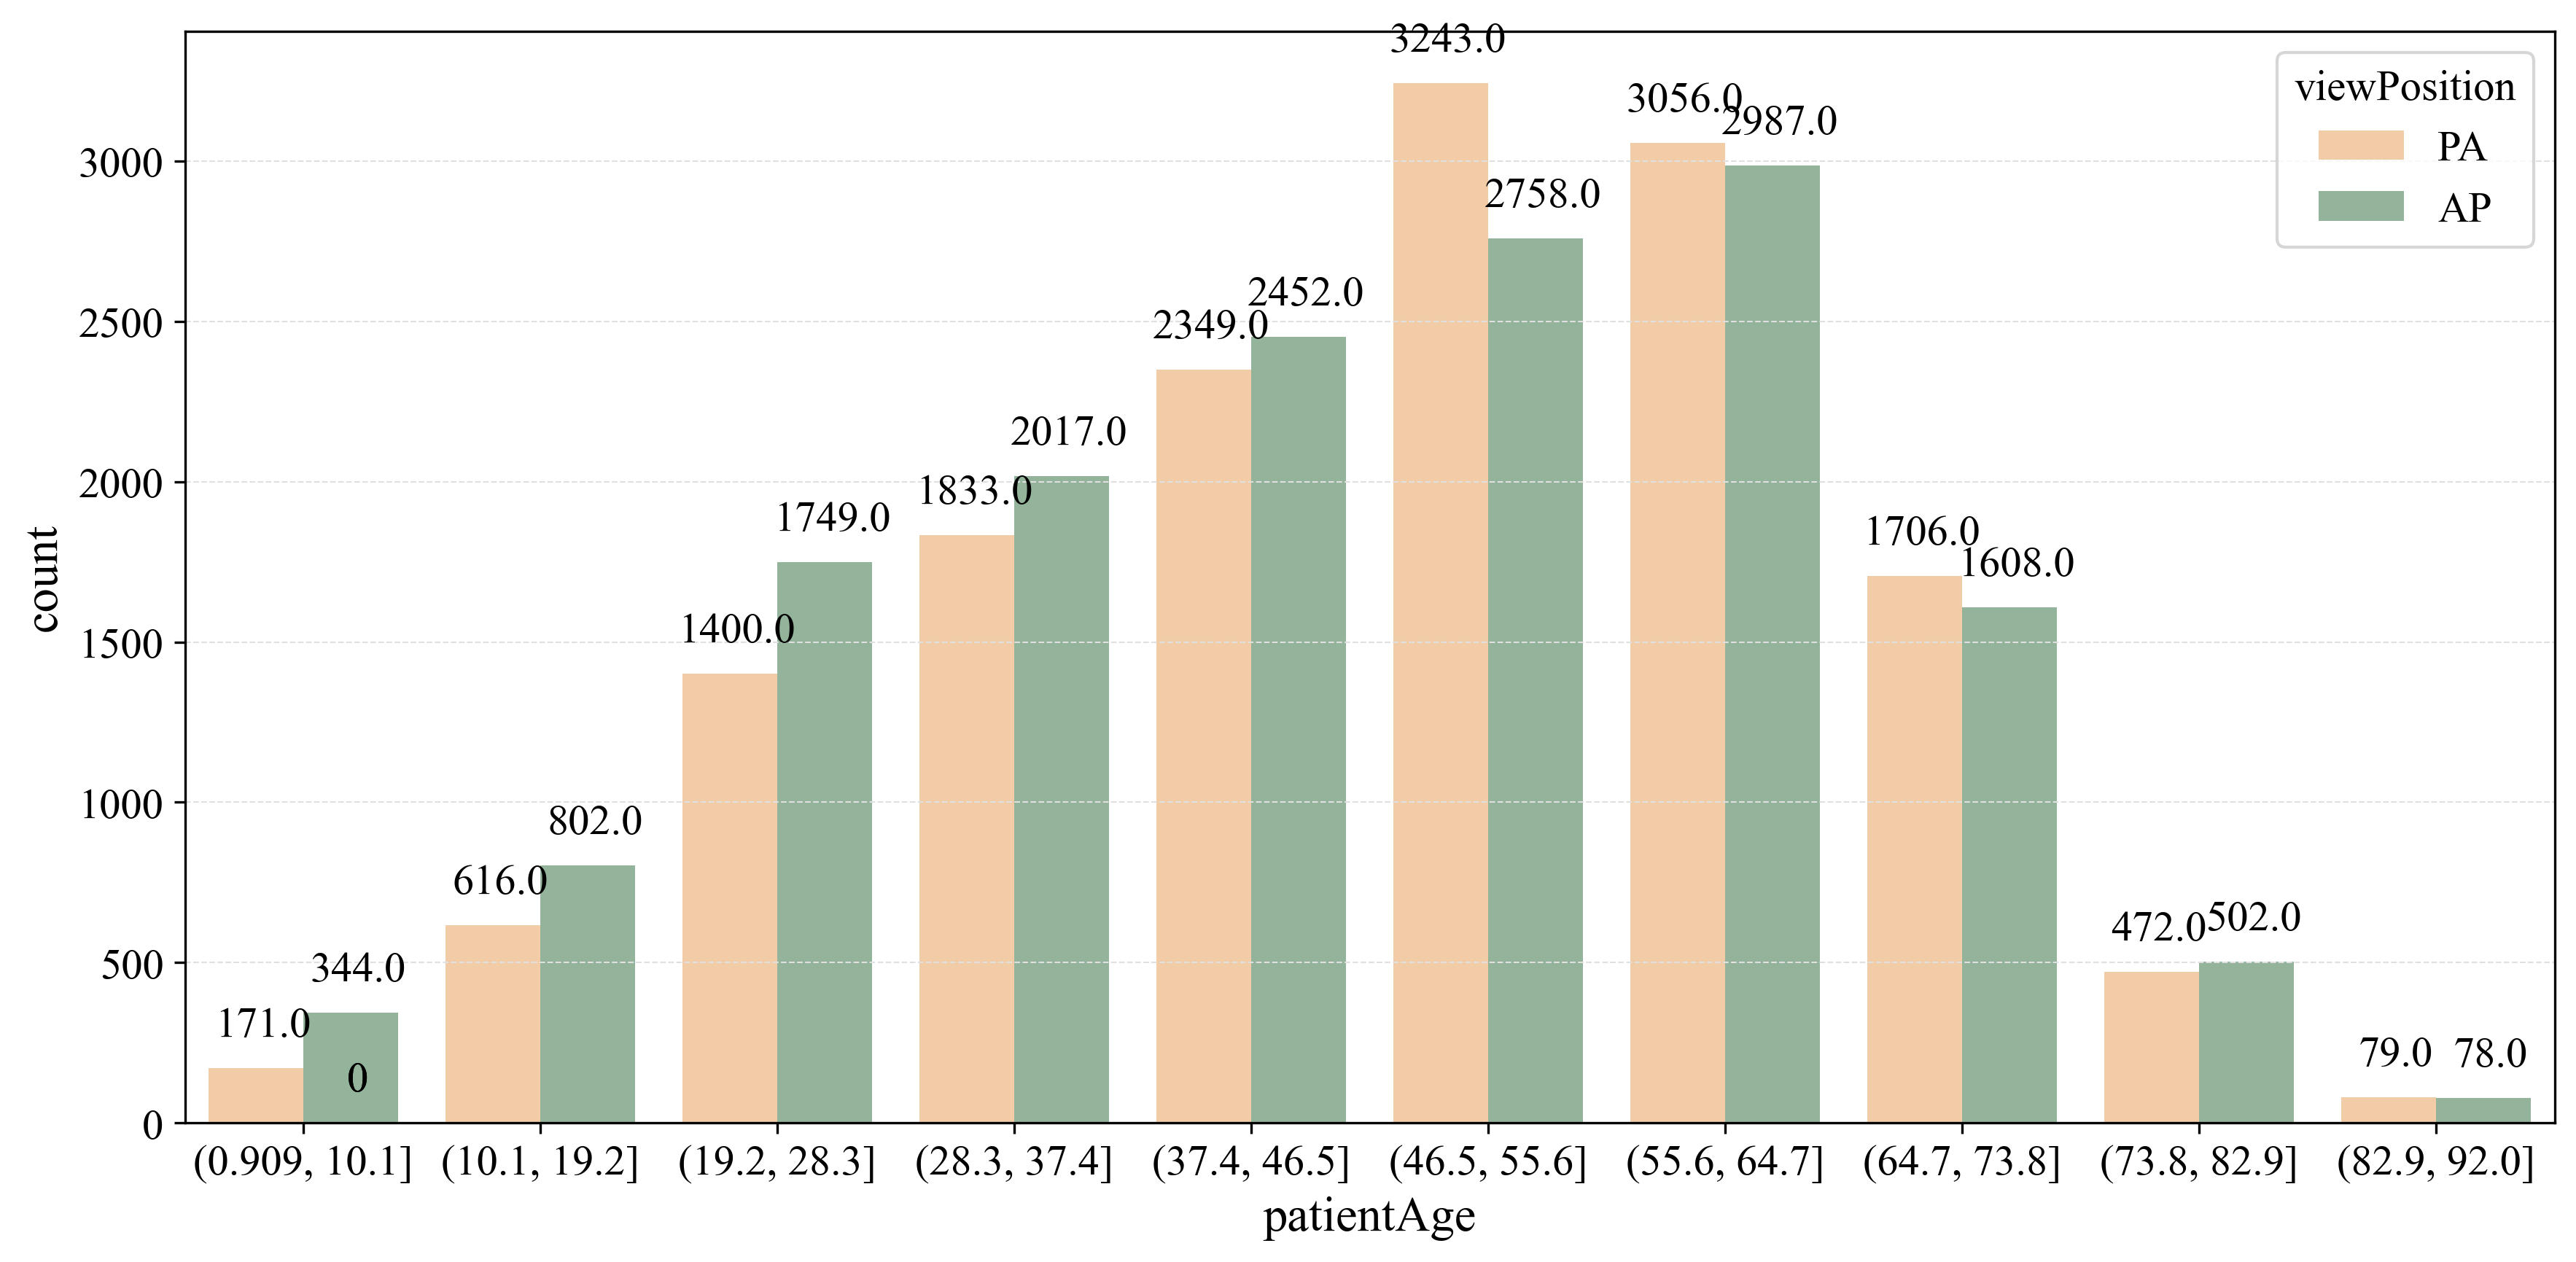
\includegraphics[width = 0.6\textwidth]{figures/Figure9.png}
        \caption{Distribution of $viewPosition$ across different age groups}
        \label{fig:cha-2 figure8}
    \end{center}
\end{figure}

There is a slight predominance of PA view positions in the age range of 45 to 65 years. The balanced distribution of PA and AP view positions indicates that the dataset includes a diverse set of imaging techniques.The PA view is slightly more common in middle-aged to older patients, which could be due to the clinical preference for PA views in routine chest radiographs. The presence of both PA and AP views ensures that the model will be trained on a variety of imaging angles, improving its generalization capability.

\subsection{Analysis of Bounding Boxes}
\label{subsec:chap2 section 1.4}

Analyzing the distribution and location of bounding boxes is essential for understanding the spatial characteristics of lung opacities within the images. The center of the bounding boxes represents the approximate location of the lung opacities, which can provide insights into common patterns and areas affected by pneumonia.

\textbf{Distribution of Bounding Box Center Across Age Groups:}

The centers of the bounding boxes are plotted for different age groups to observe any age-related patterns in the location of lung opacities. The age groups considered are: 0-25, 25-50, 50-75, and 75-100 years. Figures ~\ref{fig:cha-2 figure9} and ~\ref{fig:cha-2 figure10} illustrate the distribution of bounding box centers across different age groups.

\begin{figure}[H]
    \begin{center}
        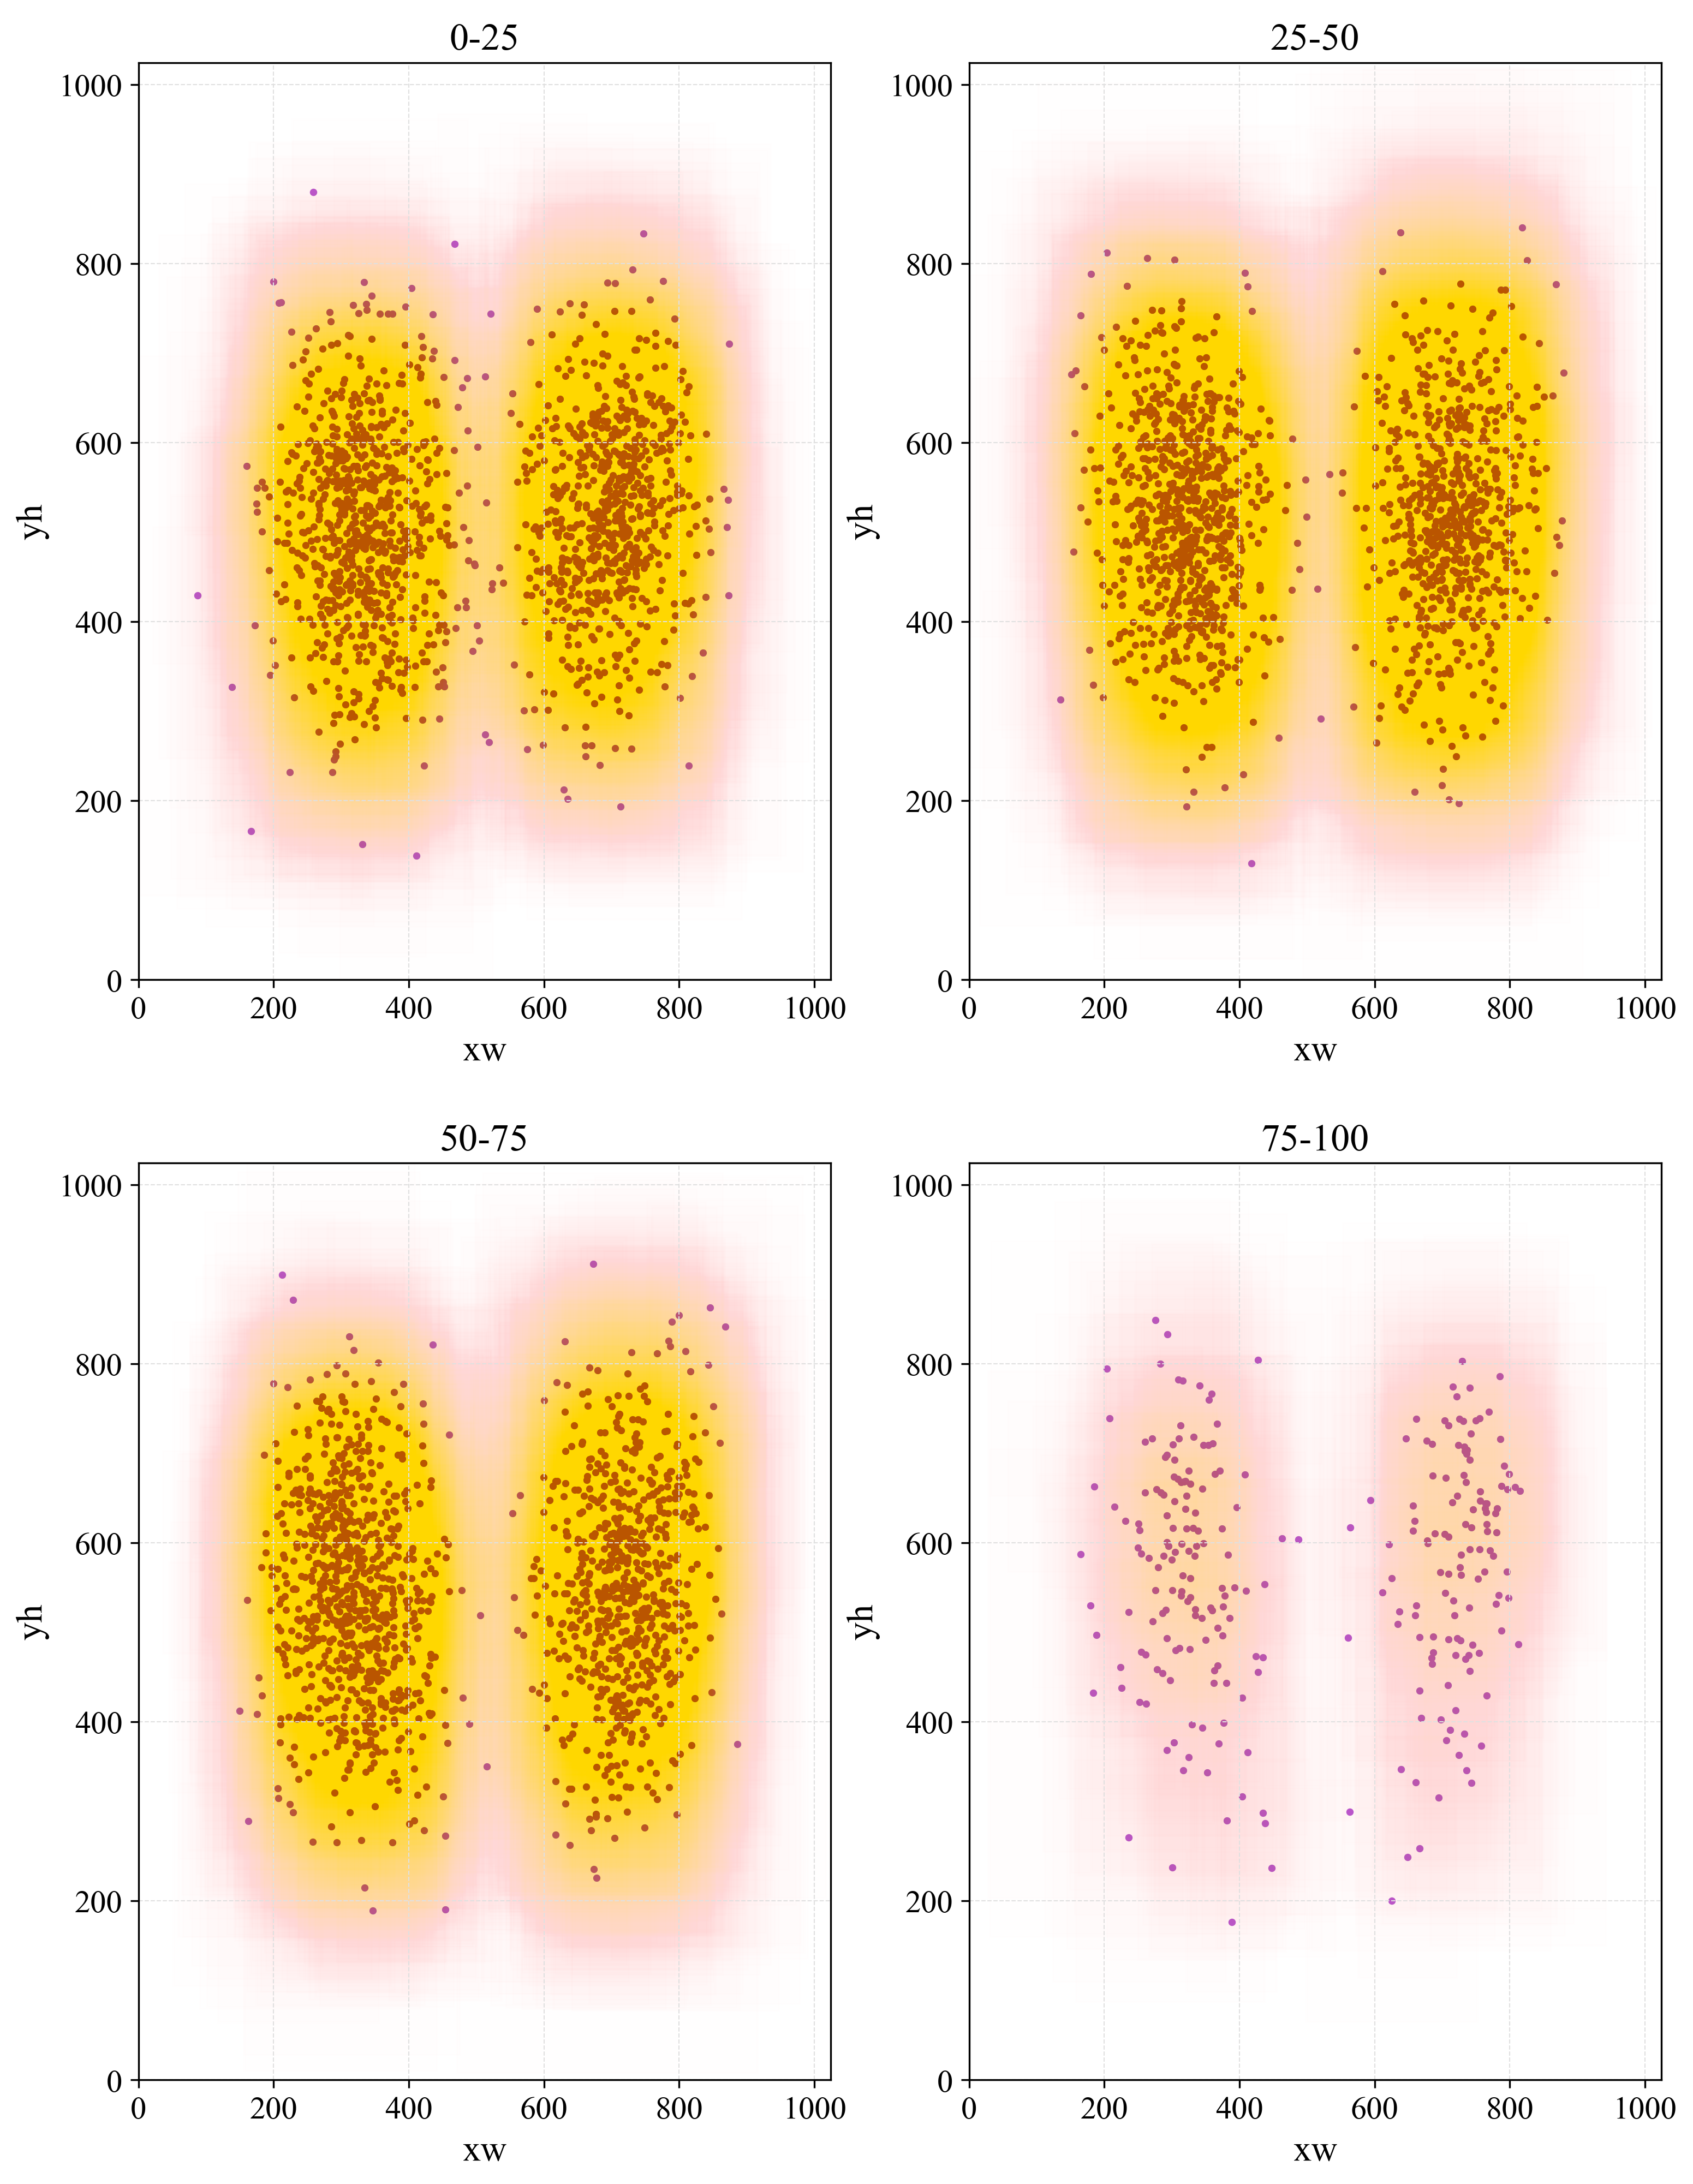
\includegraphics[width = 0.6\textwidth]{figures/Figure14.png}
        \caption{Distribution of bounding box centers across different age groups}
        \label{fig:cha-2 figure9}
    \end{center}
\end{figure}

\begin{figure}[H]
    \begin{center}
        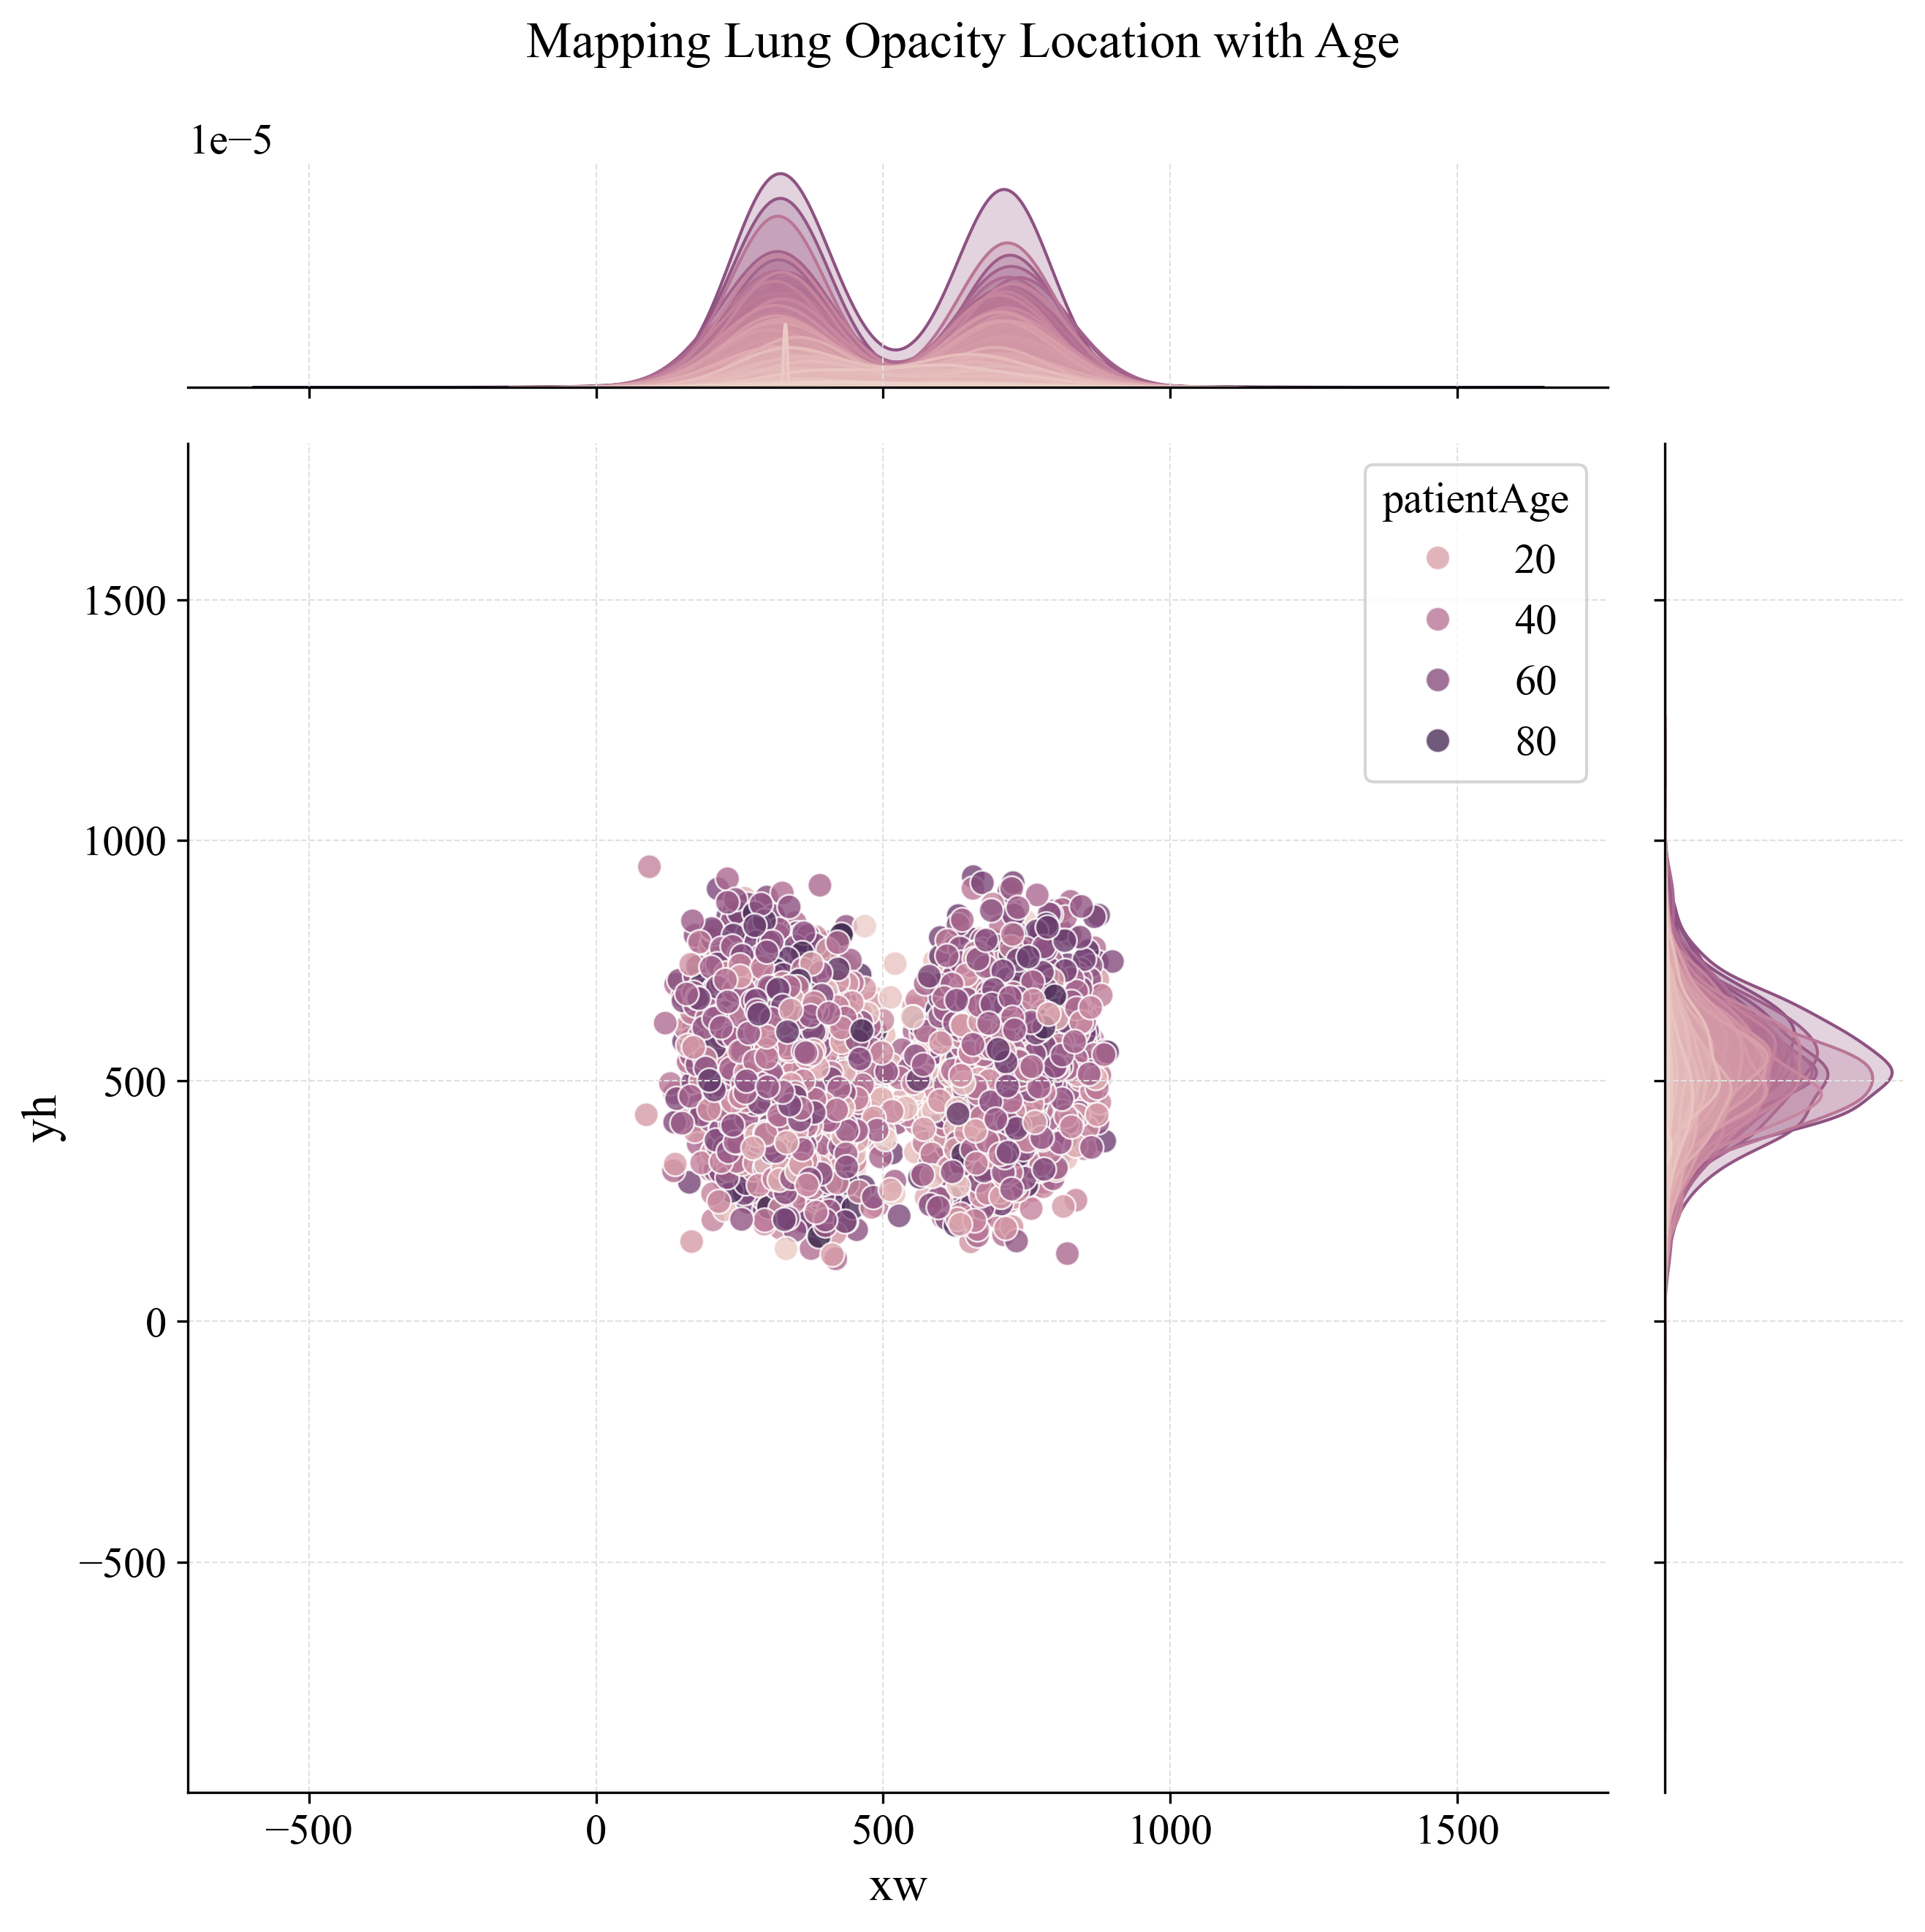
\includegraphics[width = 0.6\textwidth]{figures/Figure15.png}
        \caption{Distribution of bounding box centers across different age groups}
        \label{fig:cha-2 figure10}
    \end{center}
\end{figure}

\begin{itemize}
    \item Age 0-25: The centers of the lung opacities are relatively dispersed but show a concentration in the central region of the lungs.
    \item Age 25-50: Similar to the younger age group, there is a noticeable concentration of lung opacities in the central region, with a slight increase in dispersion.
    \item Age 50-75: The highest concentration of lung opacities is observed in this age group, with a clear pattern of opacity centers located centrally within the lungs.
    \item Age 75-100: There is a reduction in the number of lung opacities, but the central concentration pattern persists.
\end{itemize}

The Figure ~\ref{cha-2 figure10} shows combined plot of the centers of lung opacities for all ages shows a strong concentration in the central regions of the lungs. This central concentration aligns with the typical presentation of pneumonia, which often affects the lower and central lung fields. This pattern is crucial for training the model to detect pneumonia, as it indicates the regions where opacities are most likely to be found.

A similar analysis with Gender related trends is performed and the results and illustrated in Figure ~\ref{fig:cha-2 figure11} and Figure ~\ref{fig:cha-2 figure12}.

\begin{figure}[H]
    \begin{center}
        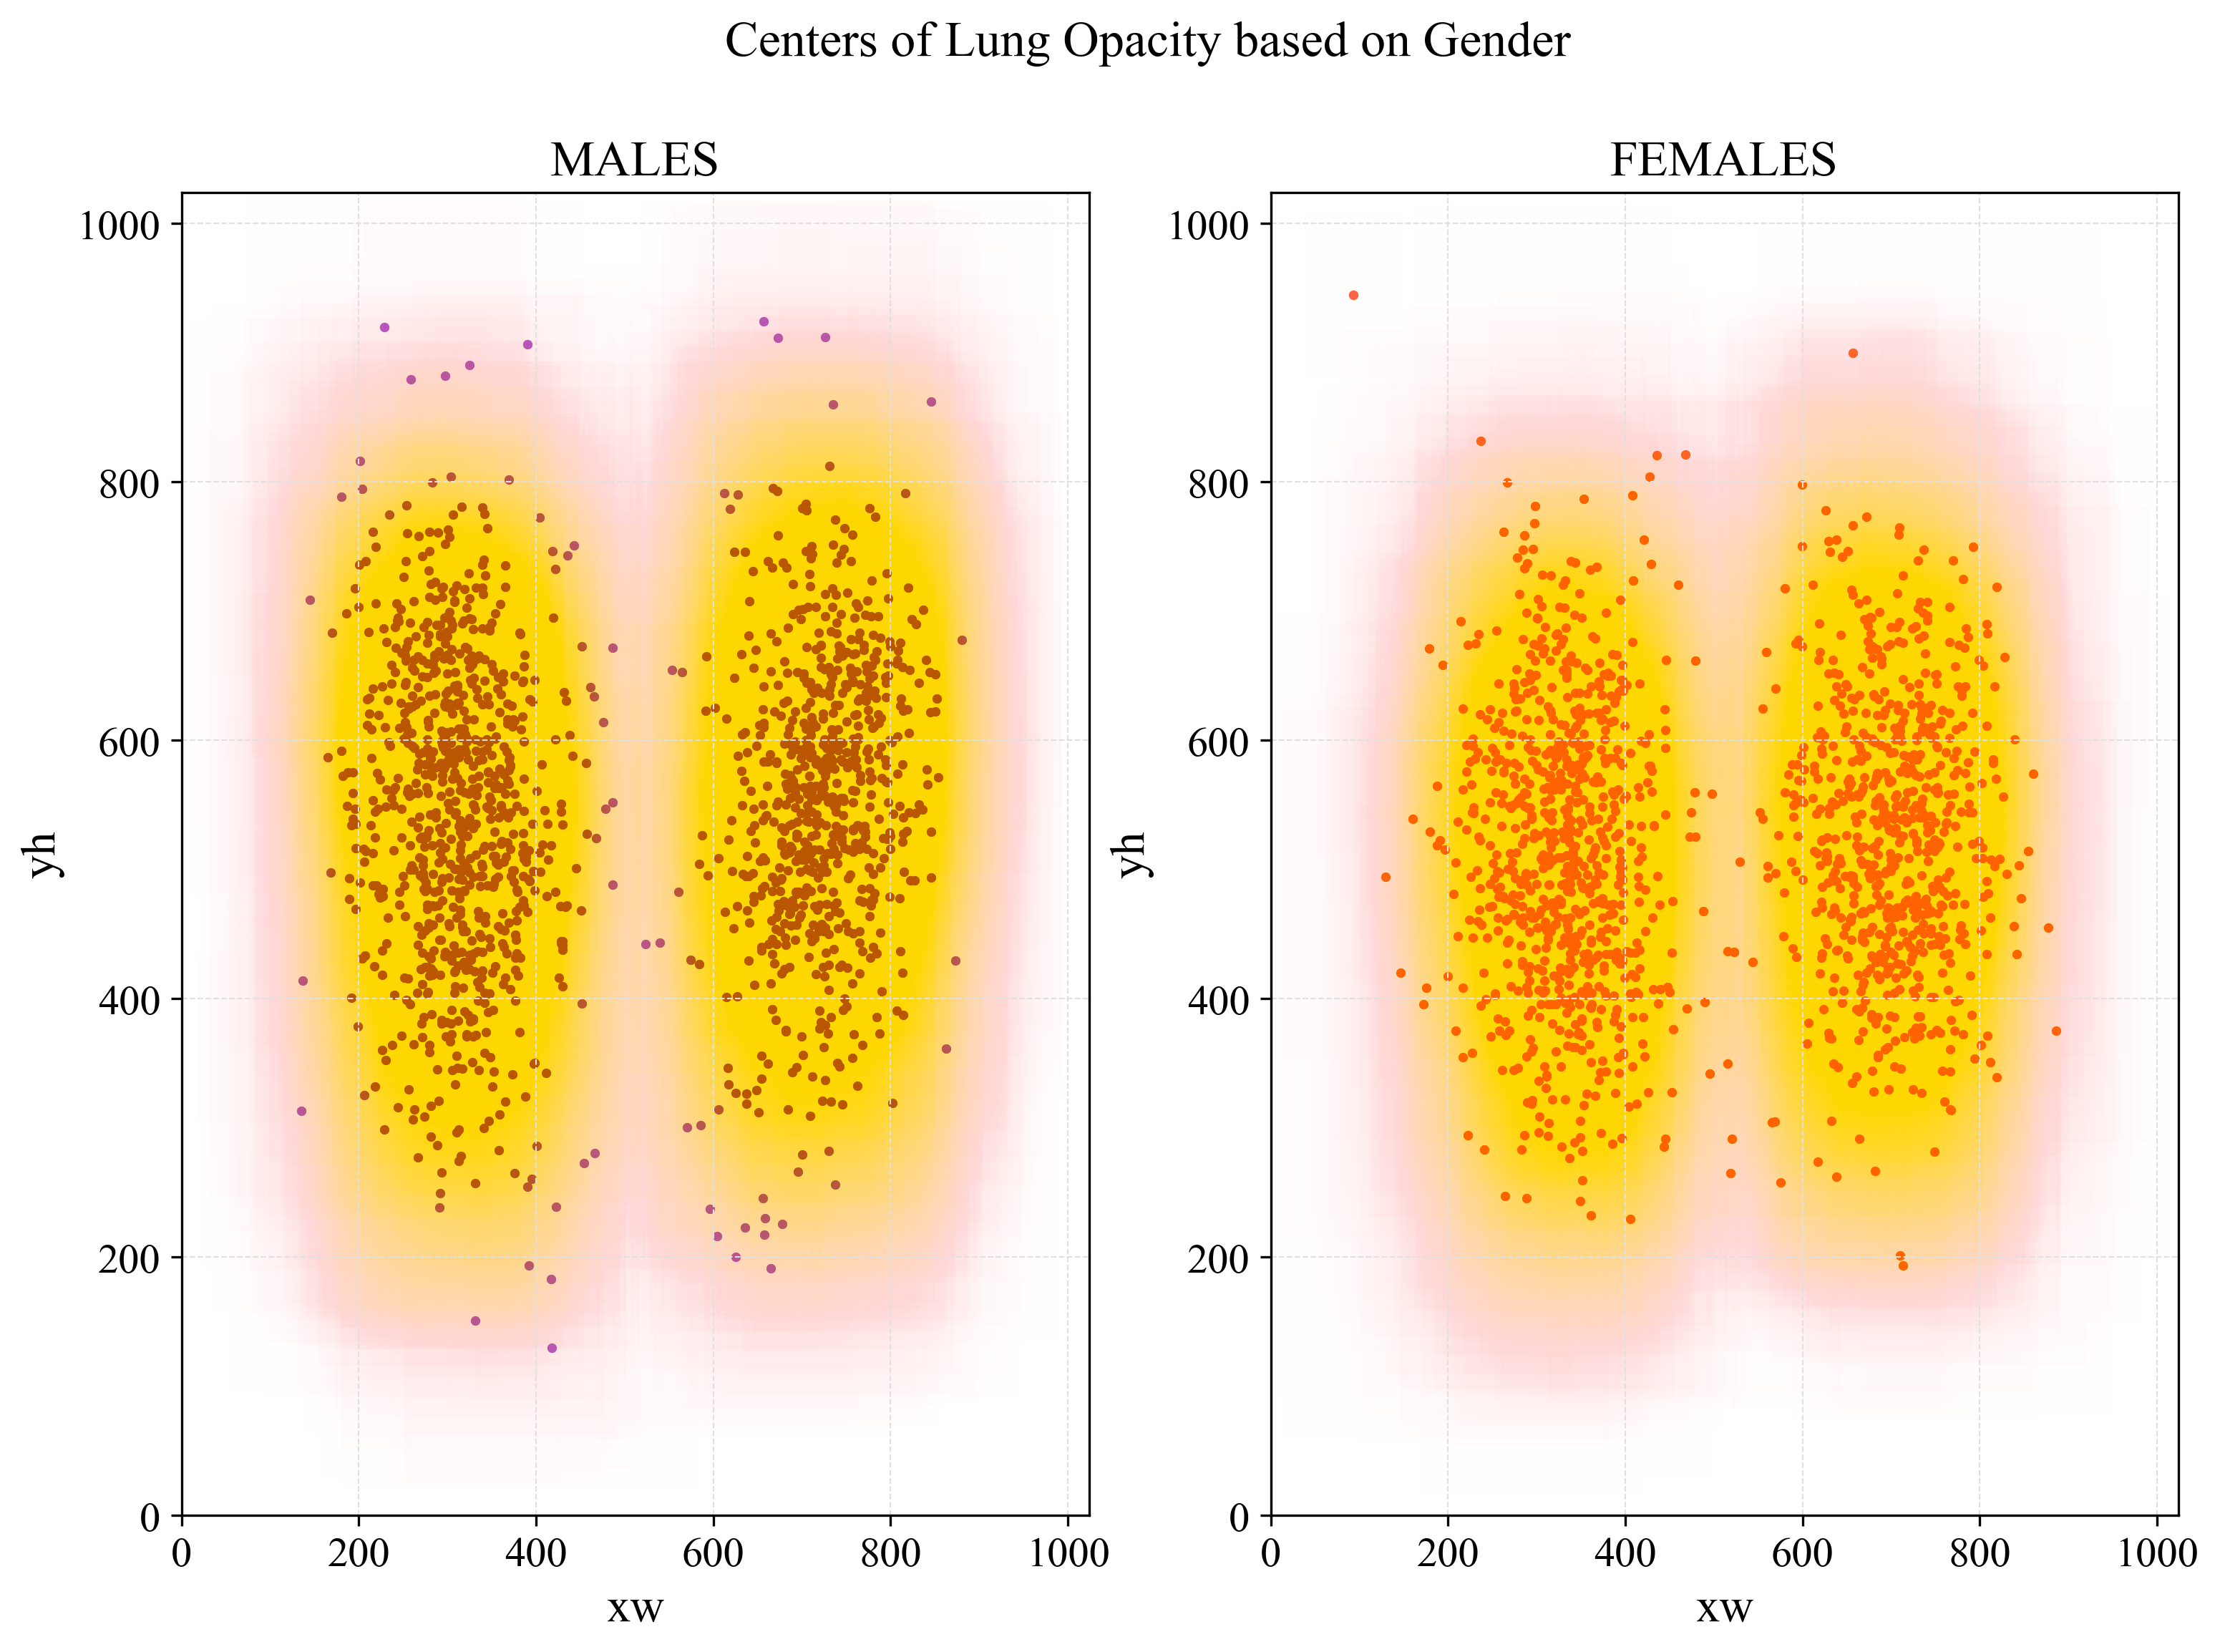
\includegraphics[width = 0.6\textwidth]{figures/Figure16.png}
        \caption{Distribution of bounding box centers across different gender groups}
        \label{fig:cha-2 figure11}
    \end{center}
\end{figure}

\begin{figure}[H]
    \begin{center}
        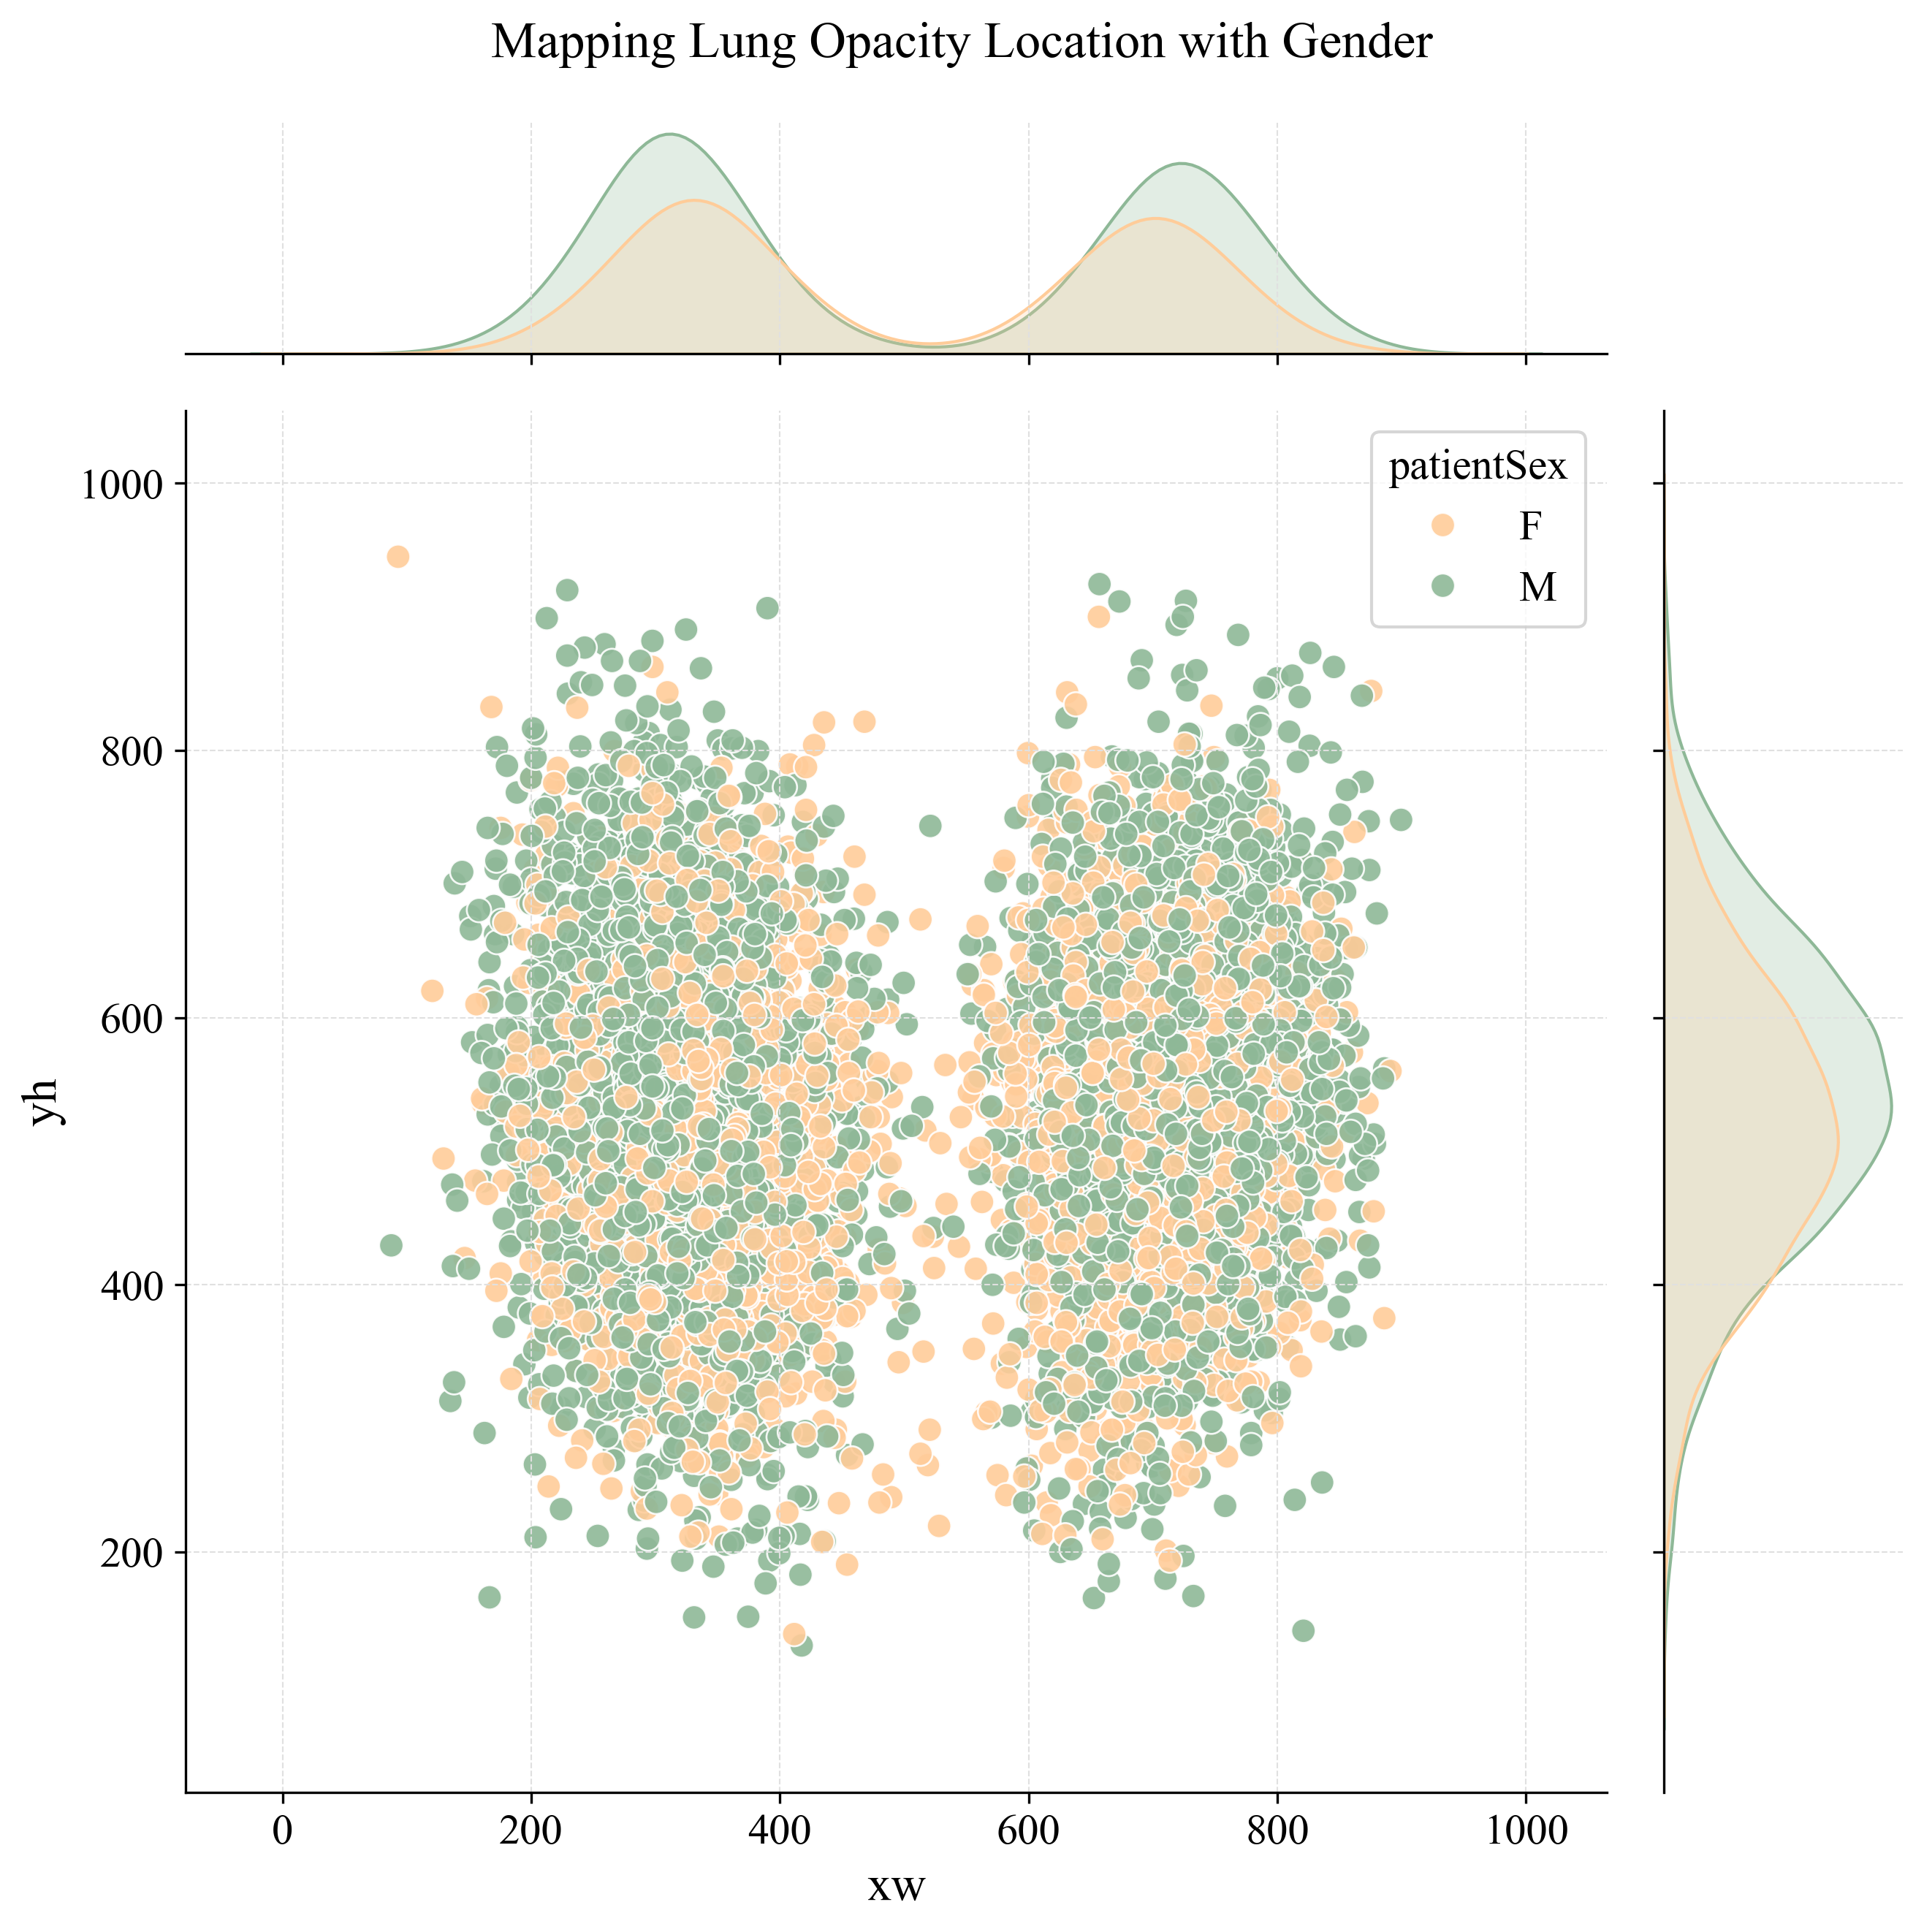
\includegraphics[width = 0.6\textwidth]{figures/Figure17.png}
        \caption{Distribution of bounding box centers across different gender groups}
        \label{fig:cha-2 figure12}
    \end{center}
\end{figure}

The analysis shows that the spatial distribution of lung opacities is similar for both male and female patients. This indicates that the model does not need to account for significant differences in the location of opacities based on gender, simplifying the training process.

A similar analysis with View Positions also shows that the spatial distribution of lung opacities is consistent across different view positions, with a central concentration pattern observed in both PA and AP views. This consistency indicates that the model can be trained effectively on images from different view positions without significant variations in the location of lung opacities. The results are illustrated in Figure ~\ref{fig:cha-2 figure13} and Figure ~\ref{fig:cha-2 figure14}.

\begin{figure}[H]
    \begin{center}
        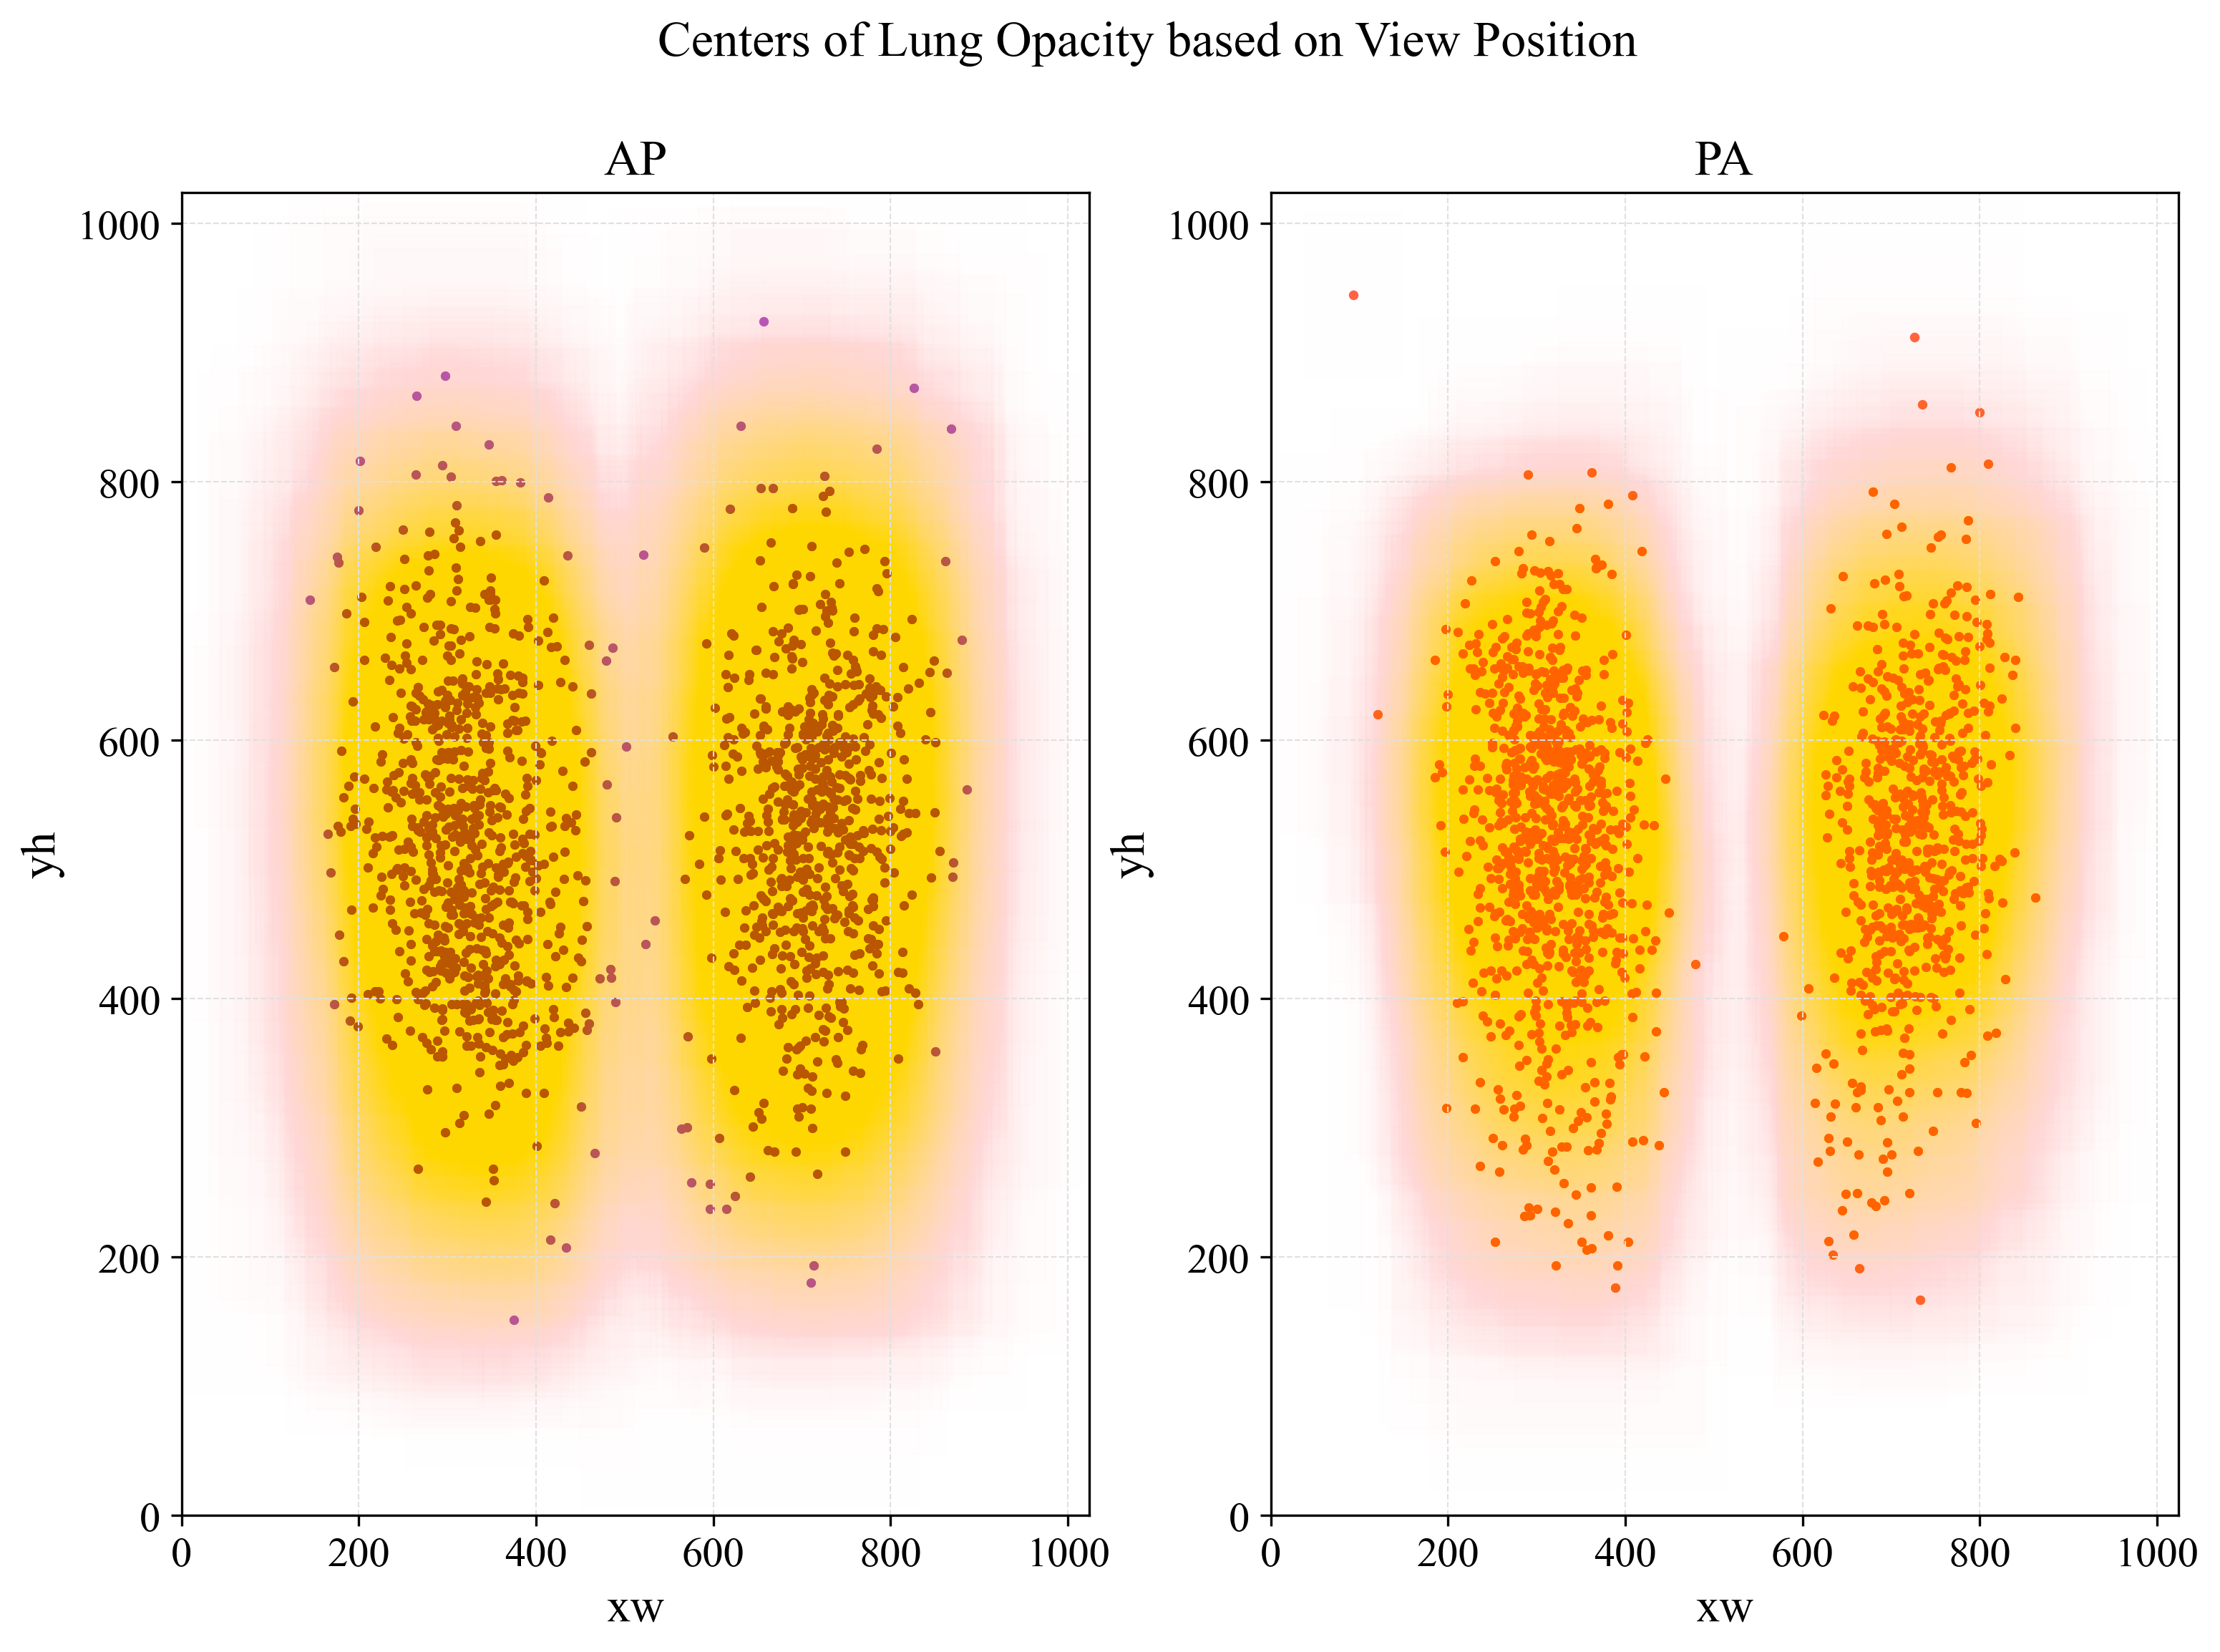
\includegraphics[width = 0.6\textwidth]{figures/Figure18.png}
        \caption{Distribution of bounding box centers across different view positions}
        \label{fig:cha-2 figure13}
    \end{center}
\end{figure}

\begin{figure}[H]
    \begin{center}
        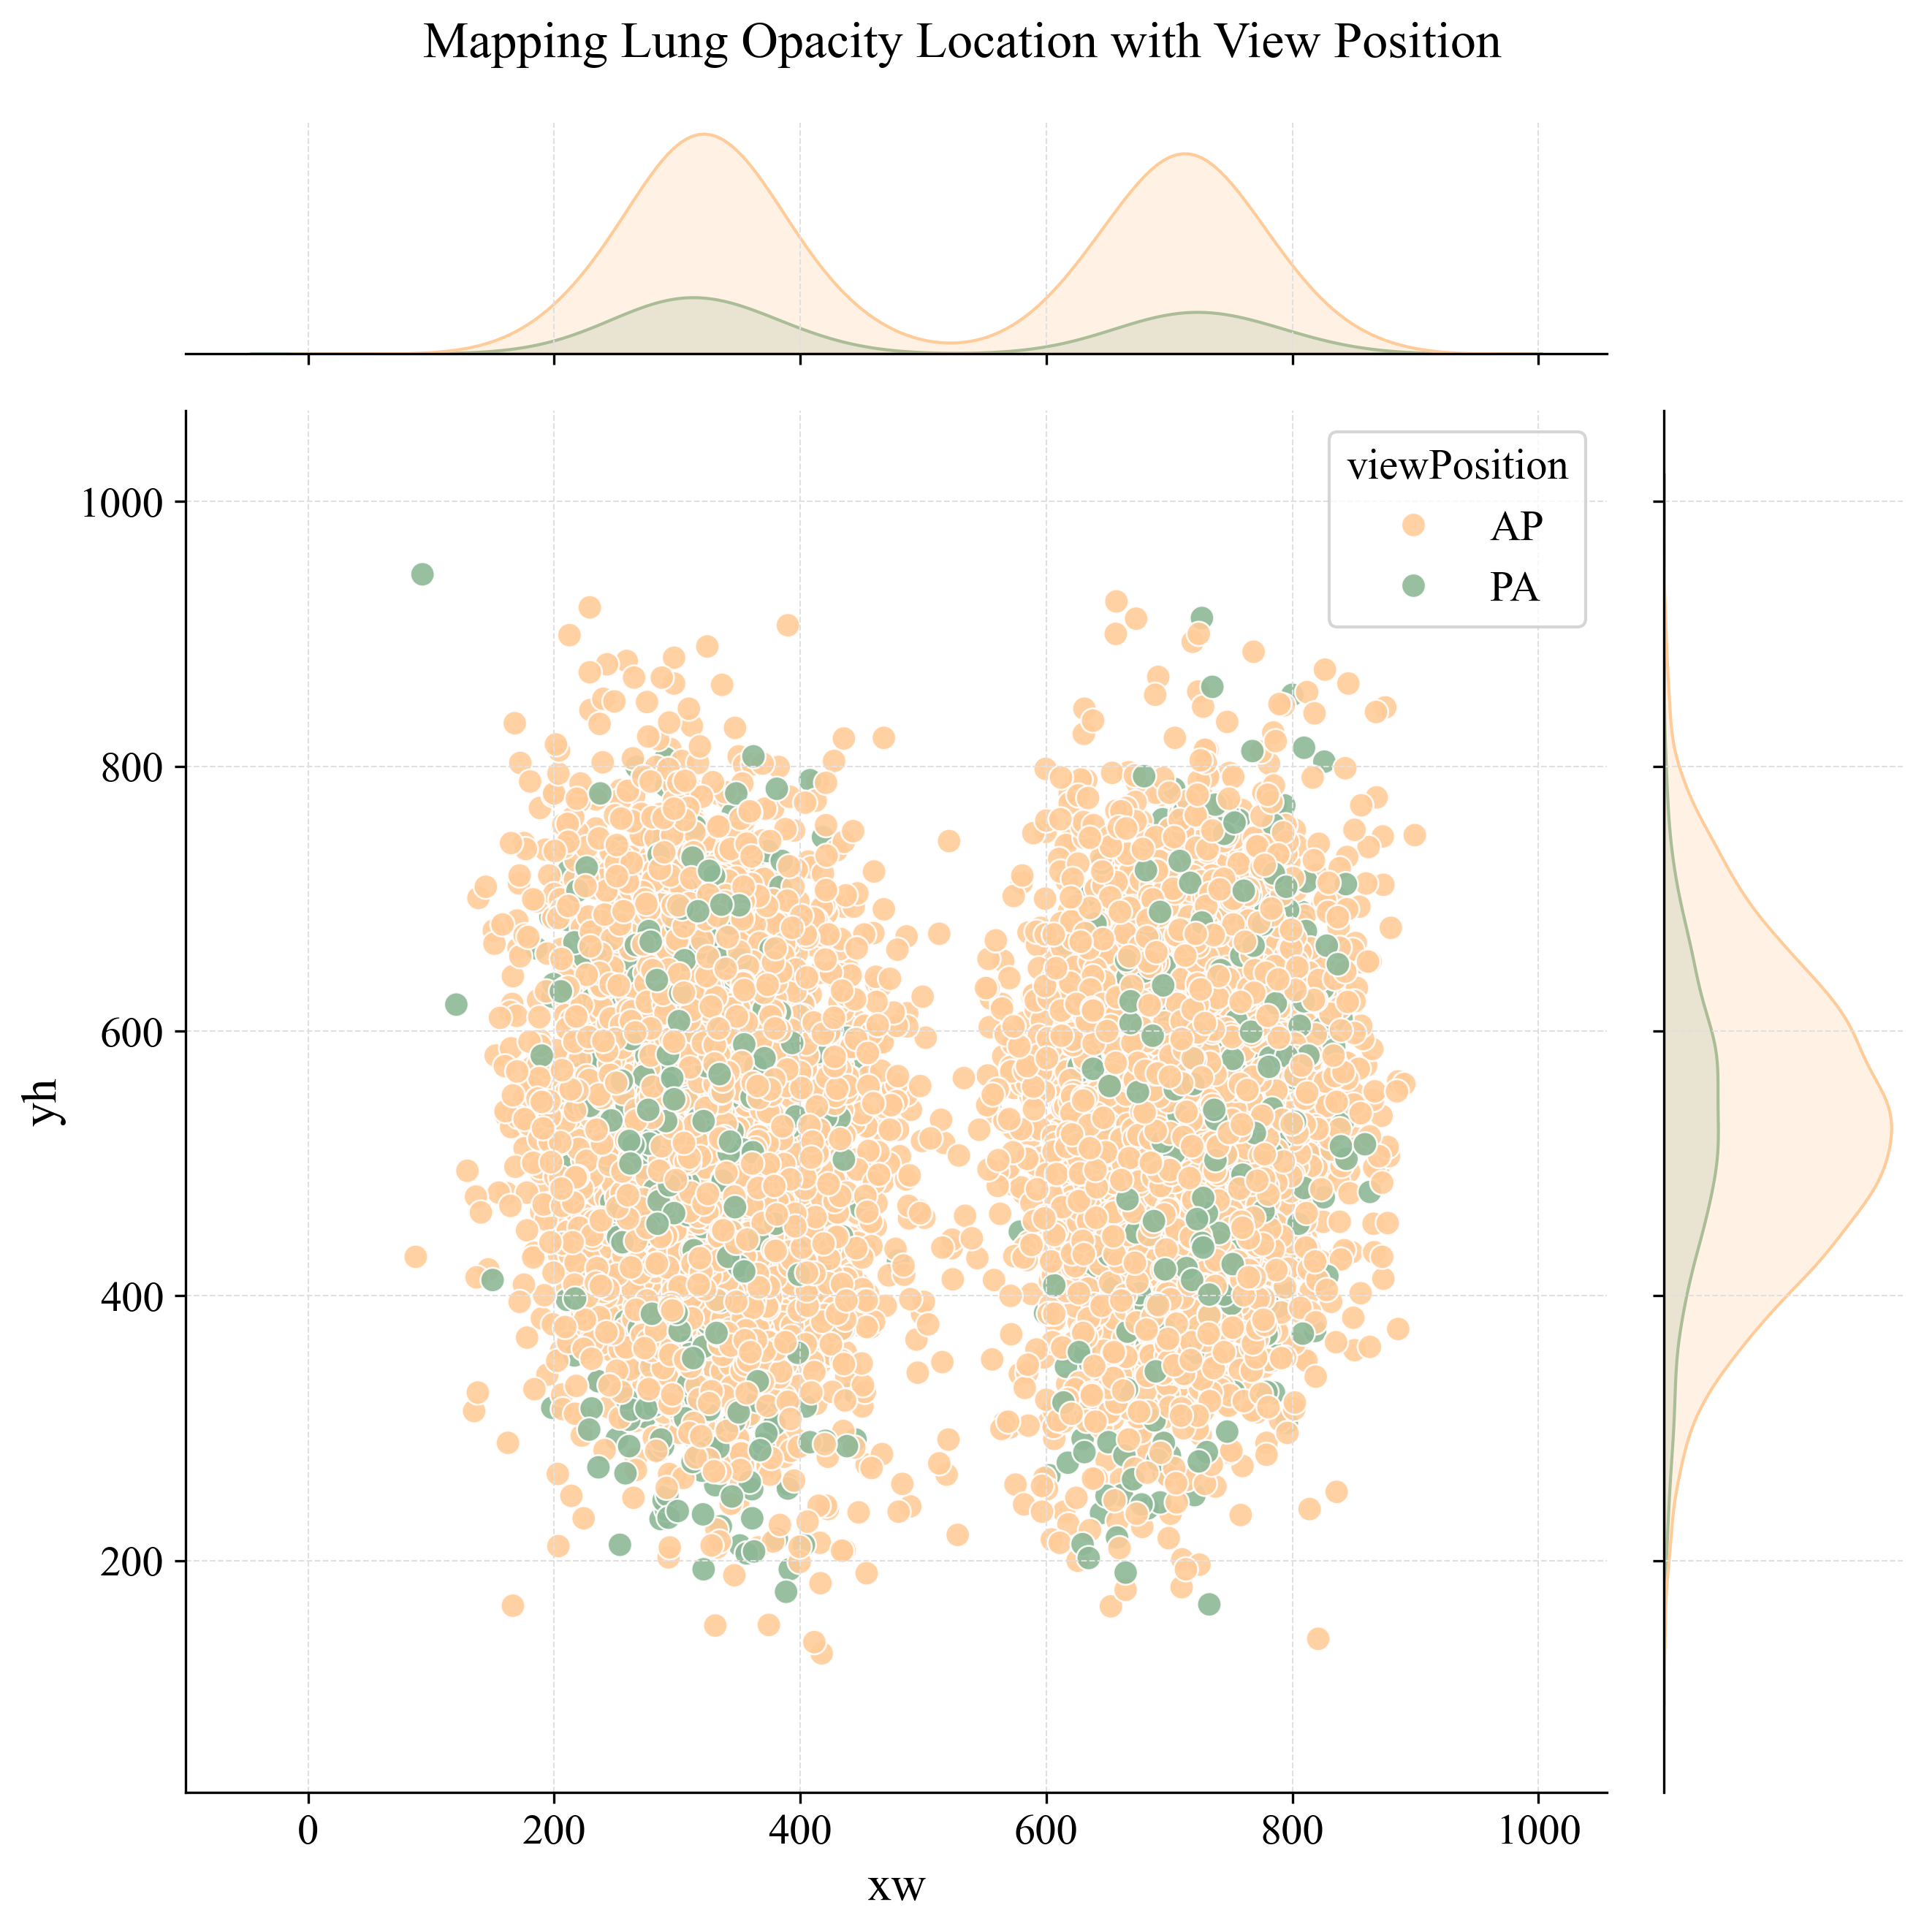
\includegraphics[width = 0.6\textwidth]{figures/Figure19.png}
        \caption{Distribution of bounding box centers across different view positions}
        \label{fig:cha-2 figure14}
    \end{center}
\end{figure}


\subsection{Handling Missing Values and Outliers}
\label{subsec:chap2 section 1.5}

It was observed that there were no missing values in the dataset. All columns, including patient IDs, bounding box coordinates, and class labels, were complete.

\textbf{Initial Outlier Detection Based on Age}
\begin{itemize}
    \item Initial Outlier Detection:
          \begin{itemize}
              \item Outliers were initially detected based on the patientAge column using a box plot analysis.
              \item The box plot revealed a few outliers in the age data, specifically ages above 100 years, which were treated as outliers and removed from the dataset.
          \end{itemize}
    \item Box Plot Analysis:
          \begin{itemize}
              \item The box plot visualization for patient age showed a few data points beyond the whiskers, indicating potential outliers.
              \item These outliers were subsequently removed to ensure a more representative age distribution.
          \end{itemize}
\end{itemize}

The box plot in Figure ~\ref{fig:cha-2 figure15} shows the distribution of patient ages and identifies outliers in the age data. Initial outliers in patient age were identified and removed. The distribution after removal of outliers is shown in Figure ~\ref{fig:cha-2 figure16}.

\begin{figure}[H]
    \begin{center}
        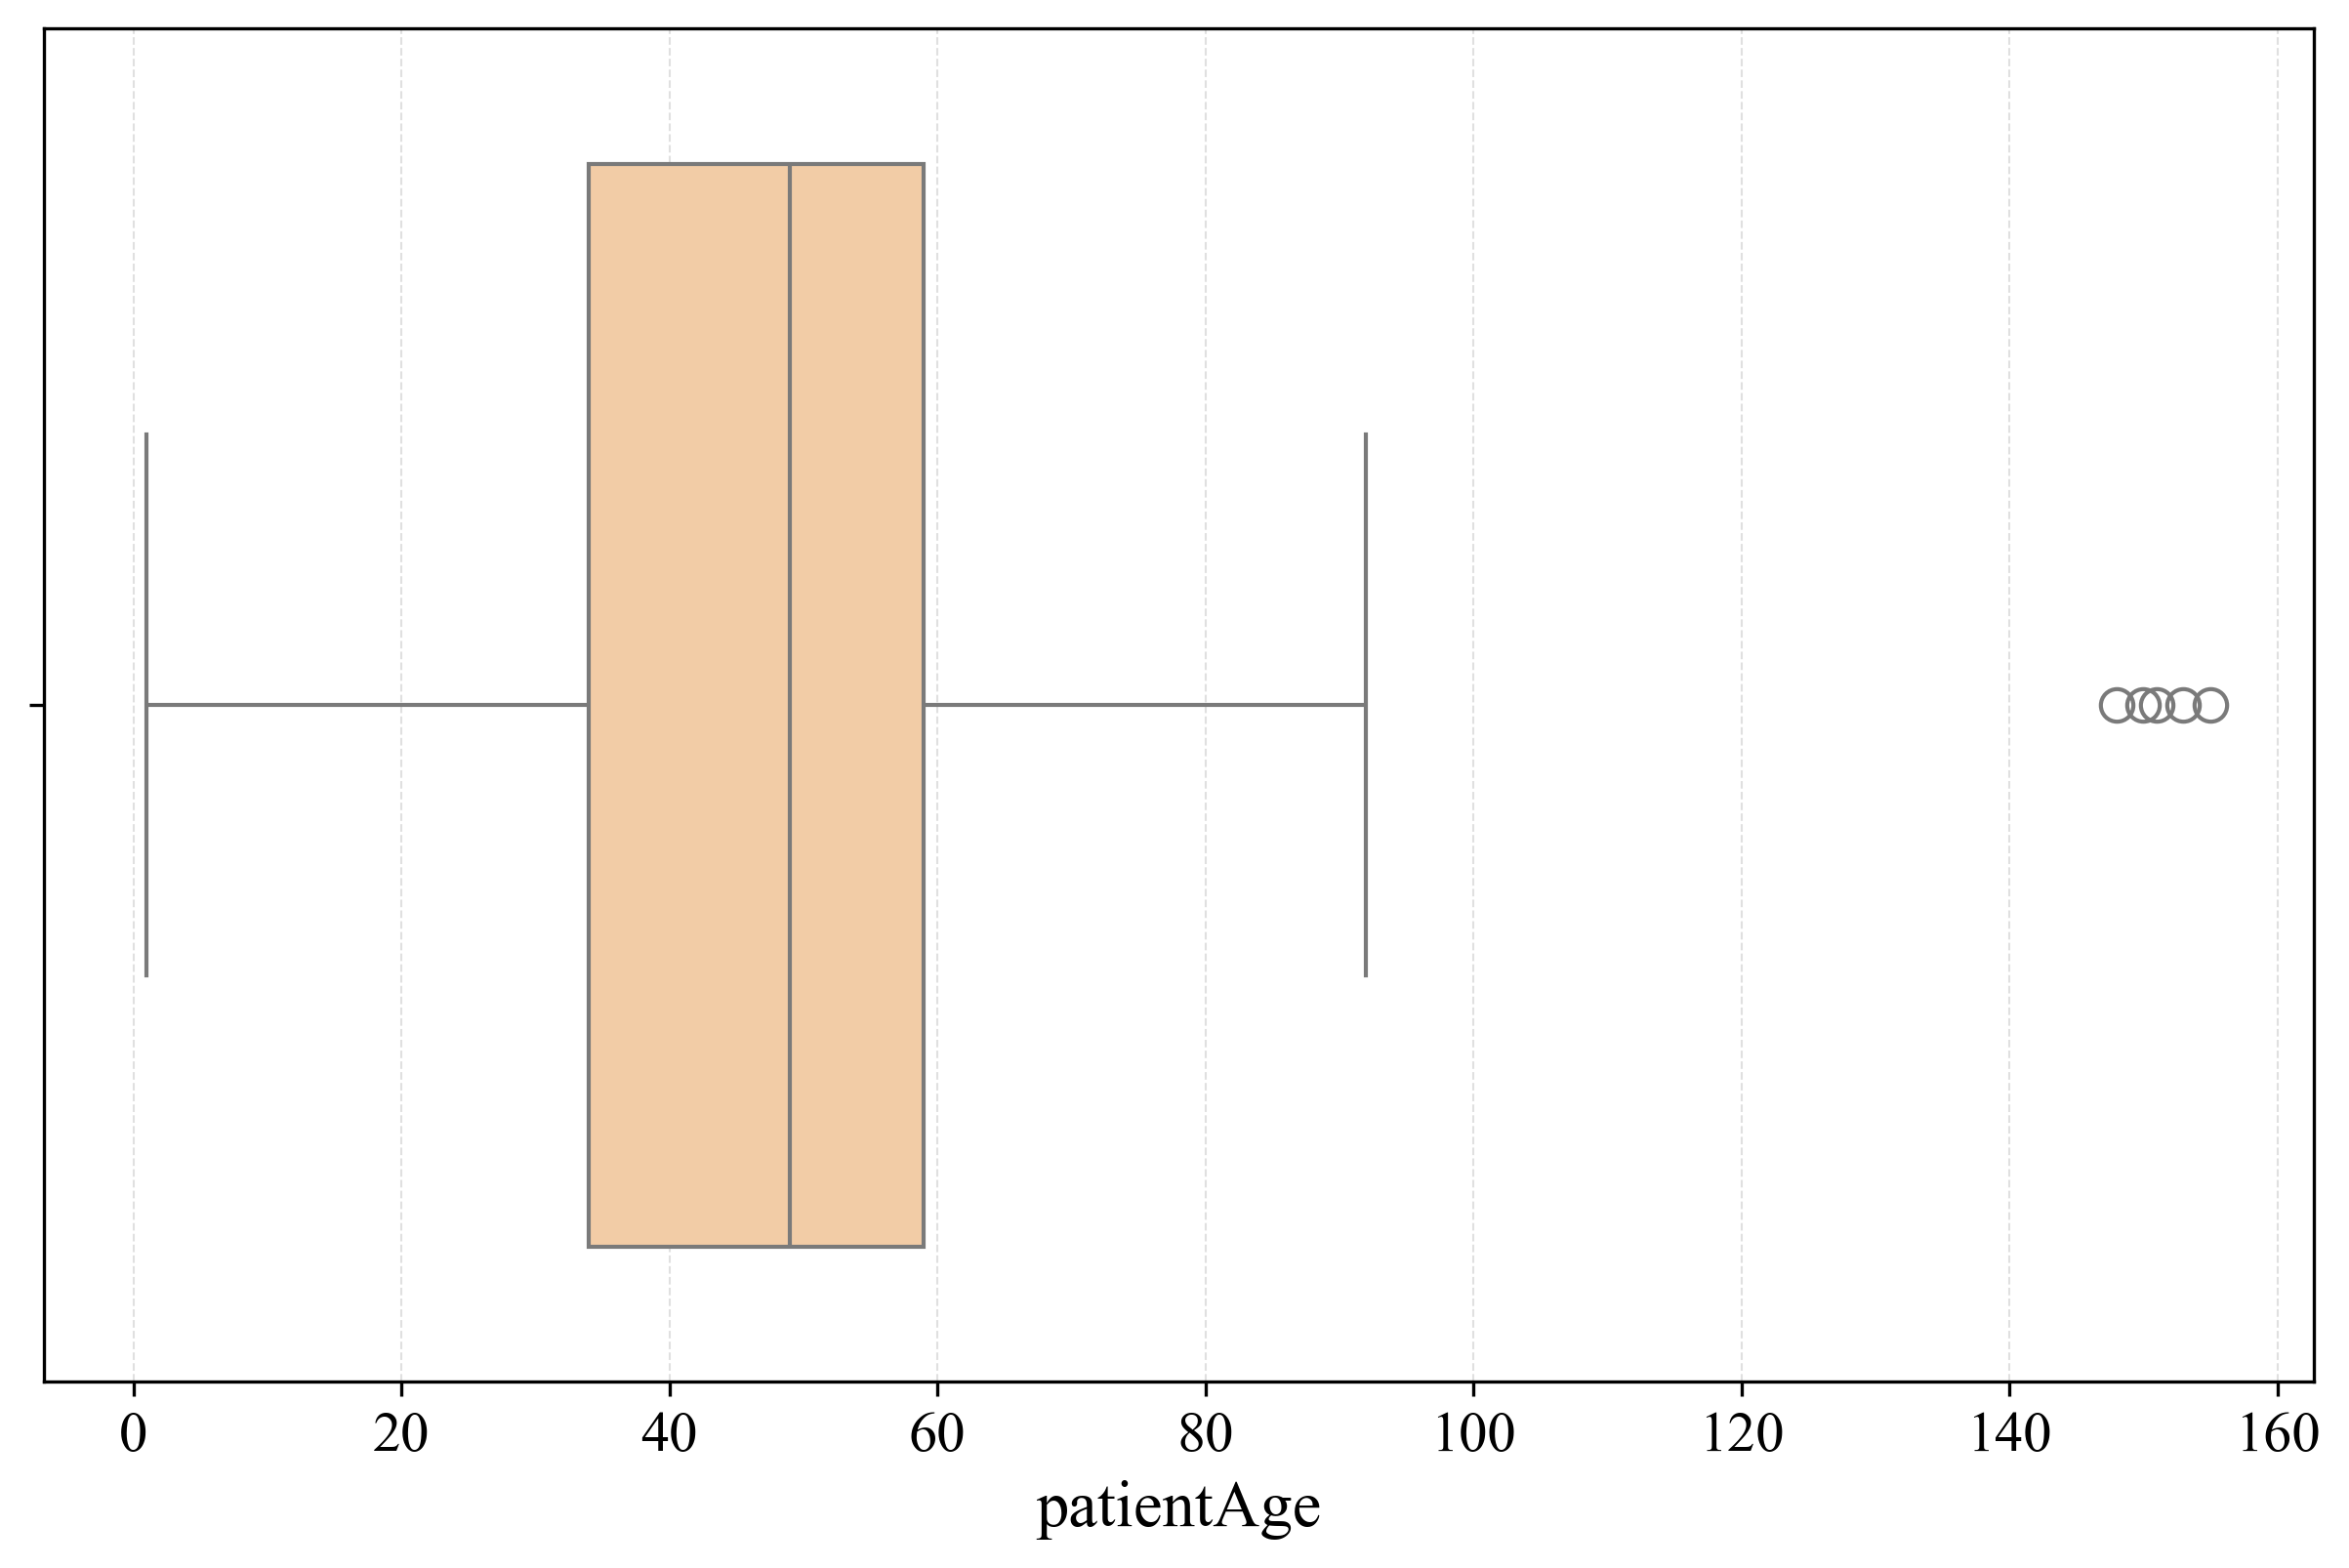
\includegraphics[width = 0.6\textwidth]{figures/Figure2.png}
        \caption{Box plot of patient age before outlier removal}
        \label{fig:cha-2 figure15}
    \end{center}
\end{figure}

\begin{figure}[H]
    \begin{center}
        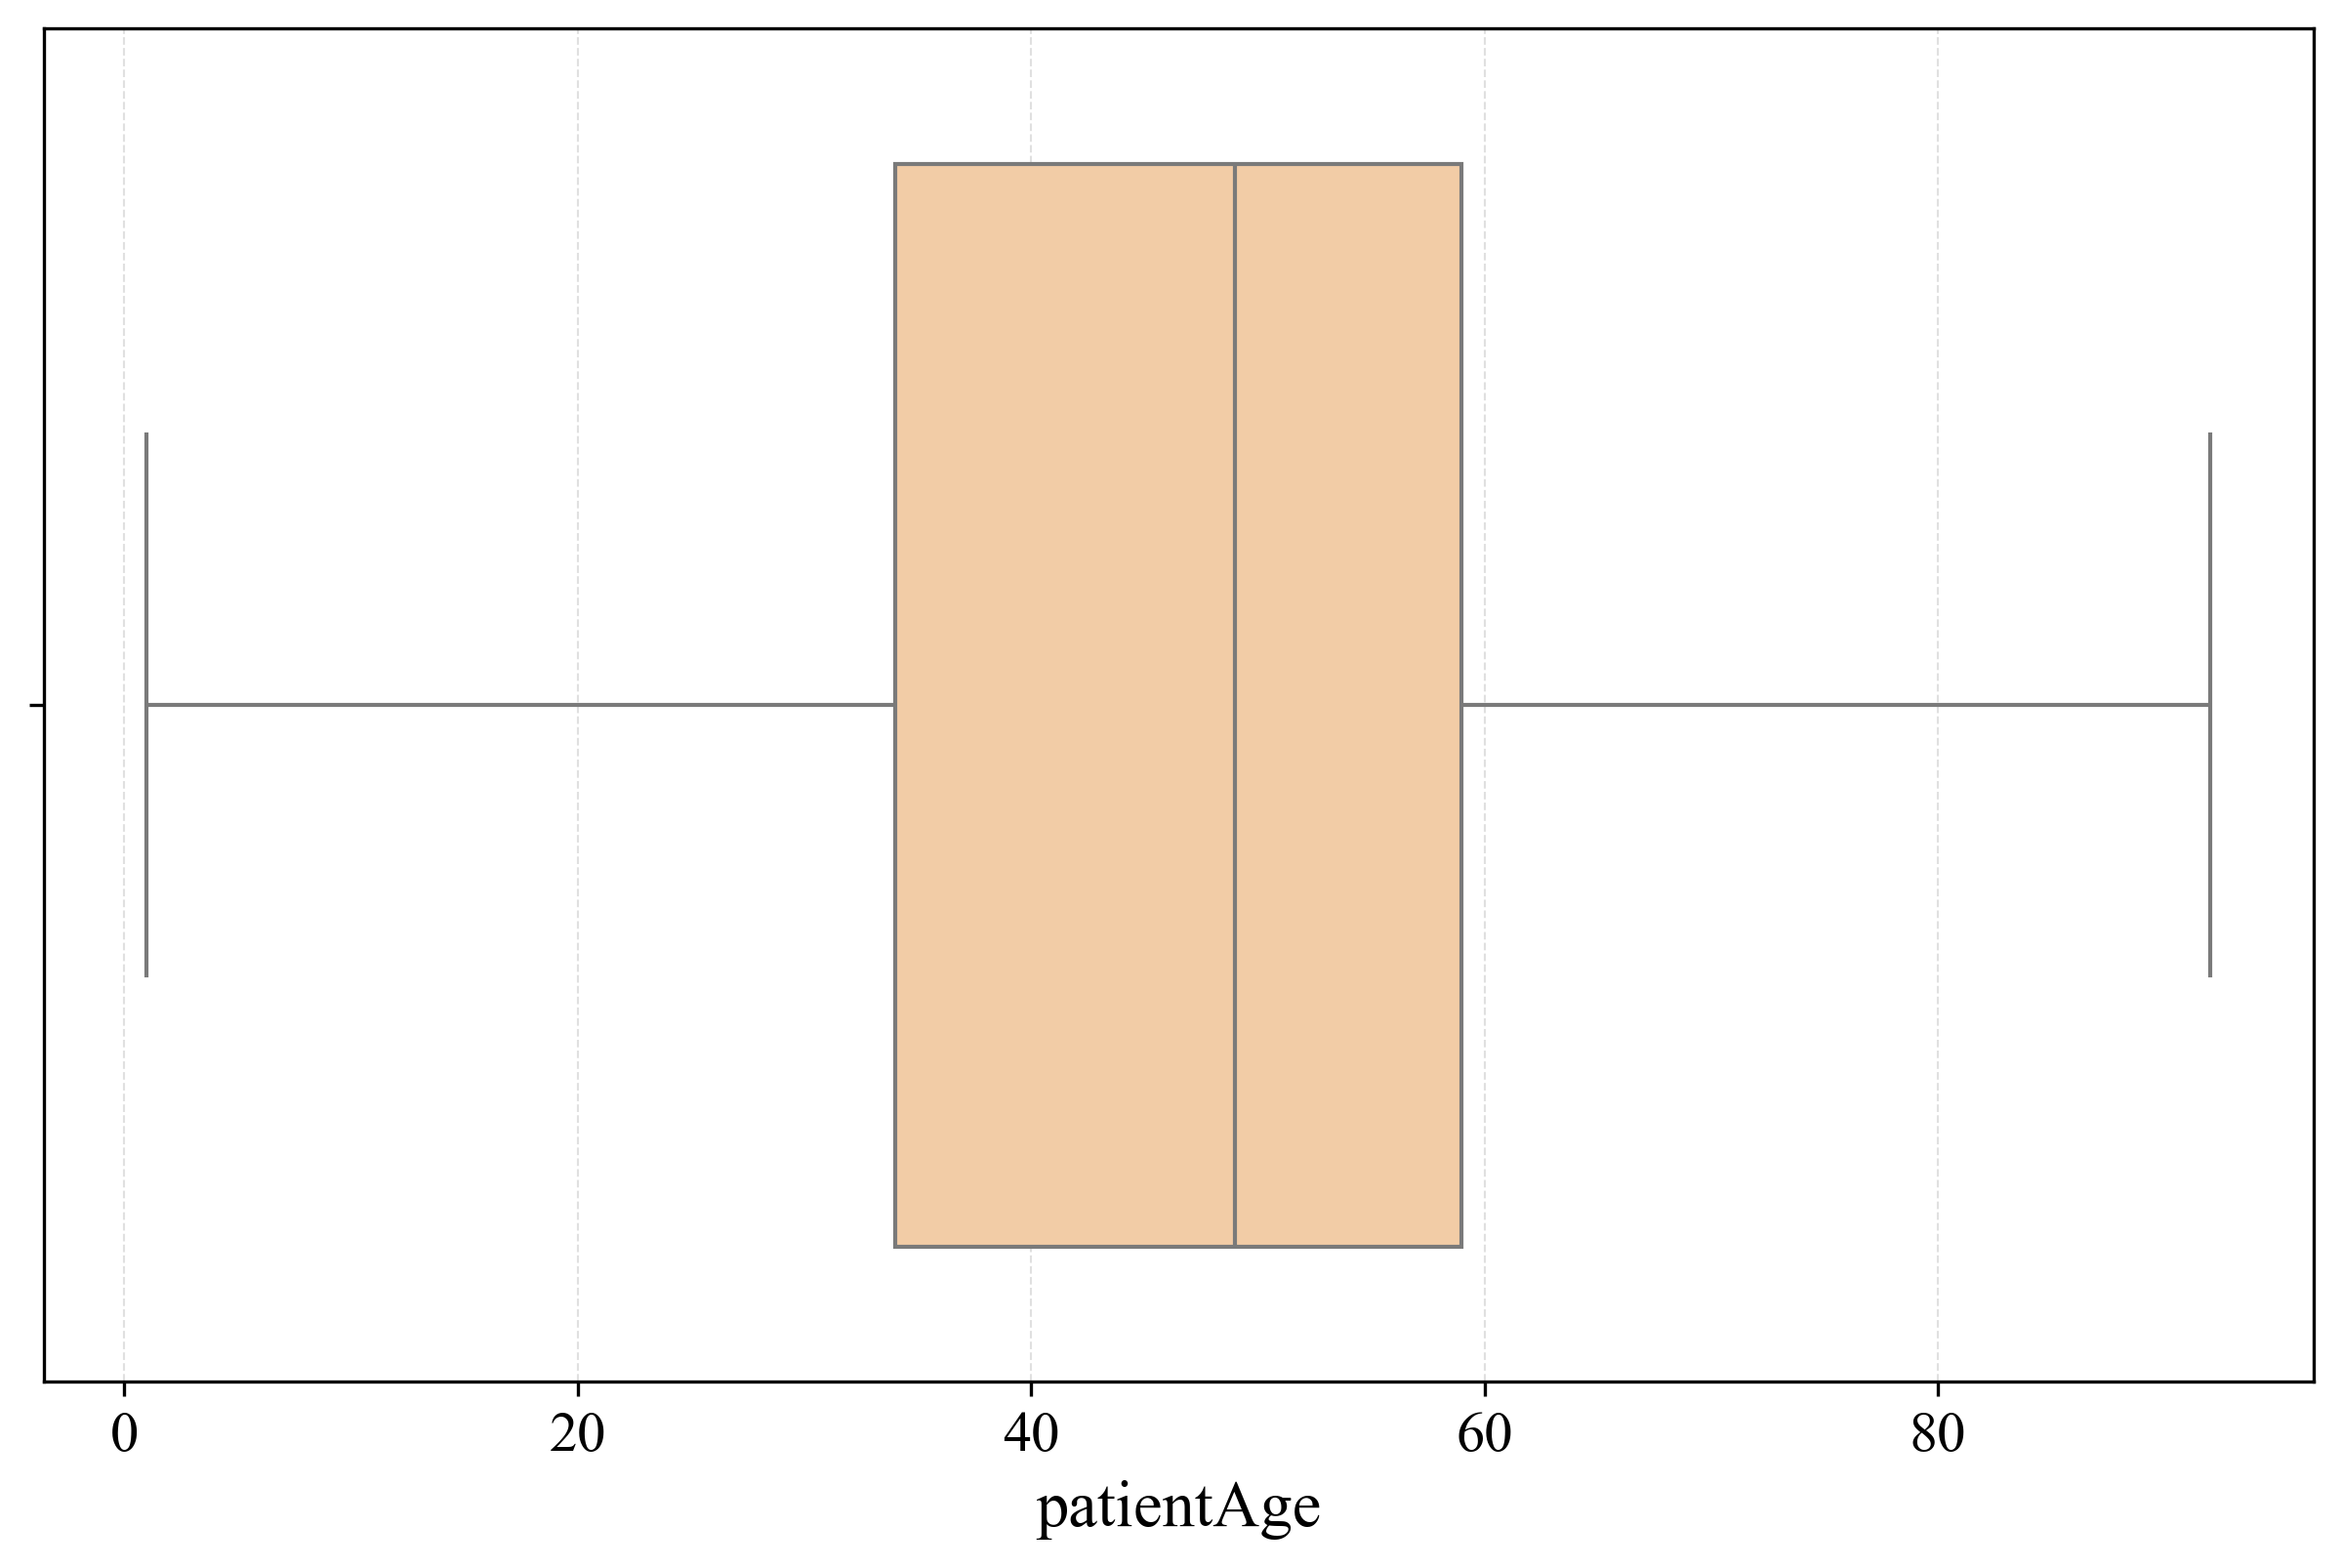
\includegraphics[width = 0.6\textwidth]{figures/Figure3.png}
        \caption{Box plot of patient age after outlier removal}
        \label{fig:cha-2 figure16}
    \end{center}
\end{figure}

\textbf{Outlier Computation based on Bounding Box Coordinates}
\begin{itemize}
    \item Outlier Computation:
          \begin{itemize}
              \item Outliers were further identified based on the location of the bounding box centers using the Gaussian Mixture Model (GMM) method.
              \item This method assumes that the data follows a mixture of Gaussian distributions and calculates the likelihood of each data point belonging to these distributions.
          \end{itemize}
    \item Outlier Detection:
          \begin{itemize}
              \item Outliers were marked as points with a low likelihood of belonging to any of the Gaussian components fitted to the data.
              \item These outliers are visualized as red crosses in the scatter plots.
          \end{itemize}
    \item Handling Outliers:
          \begin{itemize}
              \item To facilitate further analysis, two copies of the dataset were created: one with outliers and one without outliers.
              \item This allows us to compare the model performance on datasets with and without outliers and understand the impact of outliers on the model's accuracy and robustness.
          \end{itemize}
\end{itemize}

The scatter plot in Figure ~\ref{fig:cha-2 figure17} shows the centers of the bounding boxes, with outliers marked as red crosses. The initial GMM treatment identified outliers and removed them. The second scatter plot in Figure ~\ref{fig:cha-2 figure18} shows the distribution of bounding box centers after outlier removal. A second GMM analysis shows that there are a few more new outliers which are removed and the final distribution is shown in Figure ~\ref{fig:cha-2 figure19}.

\begin{figure}[H]
    \begin{center}
        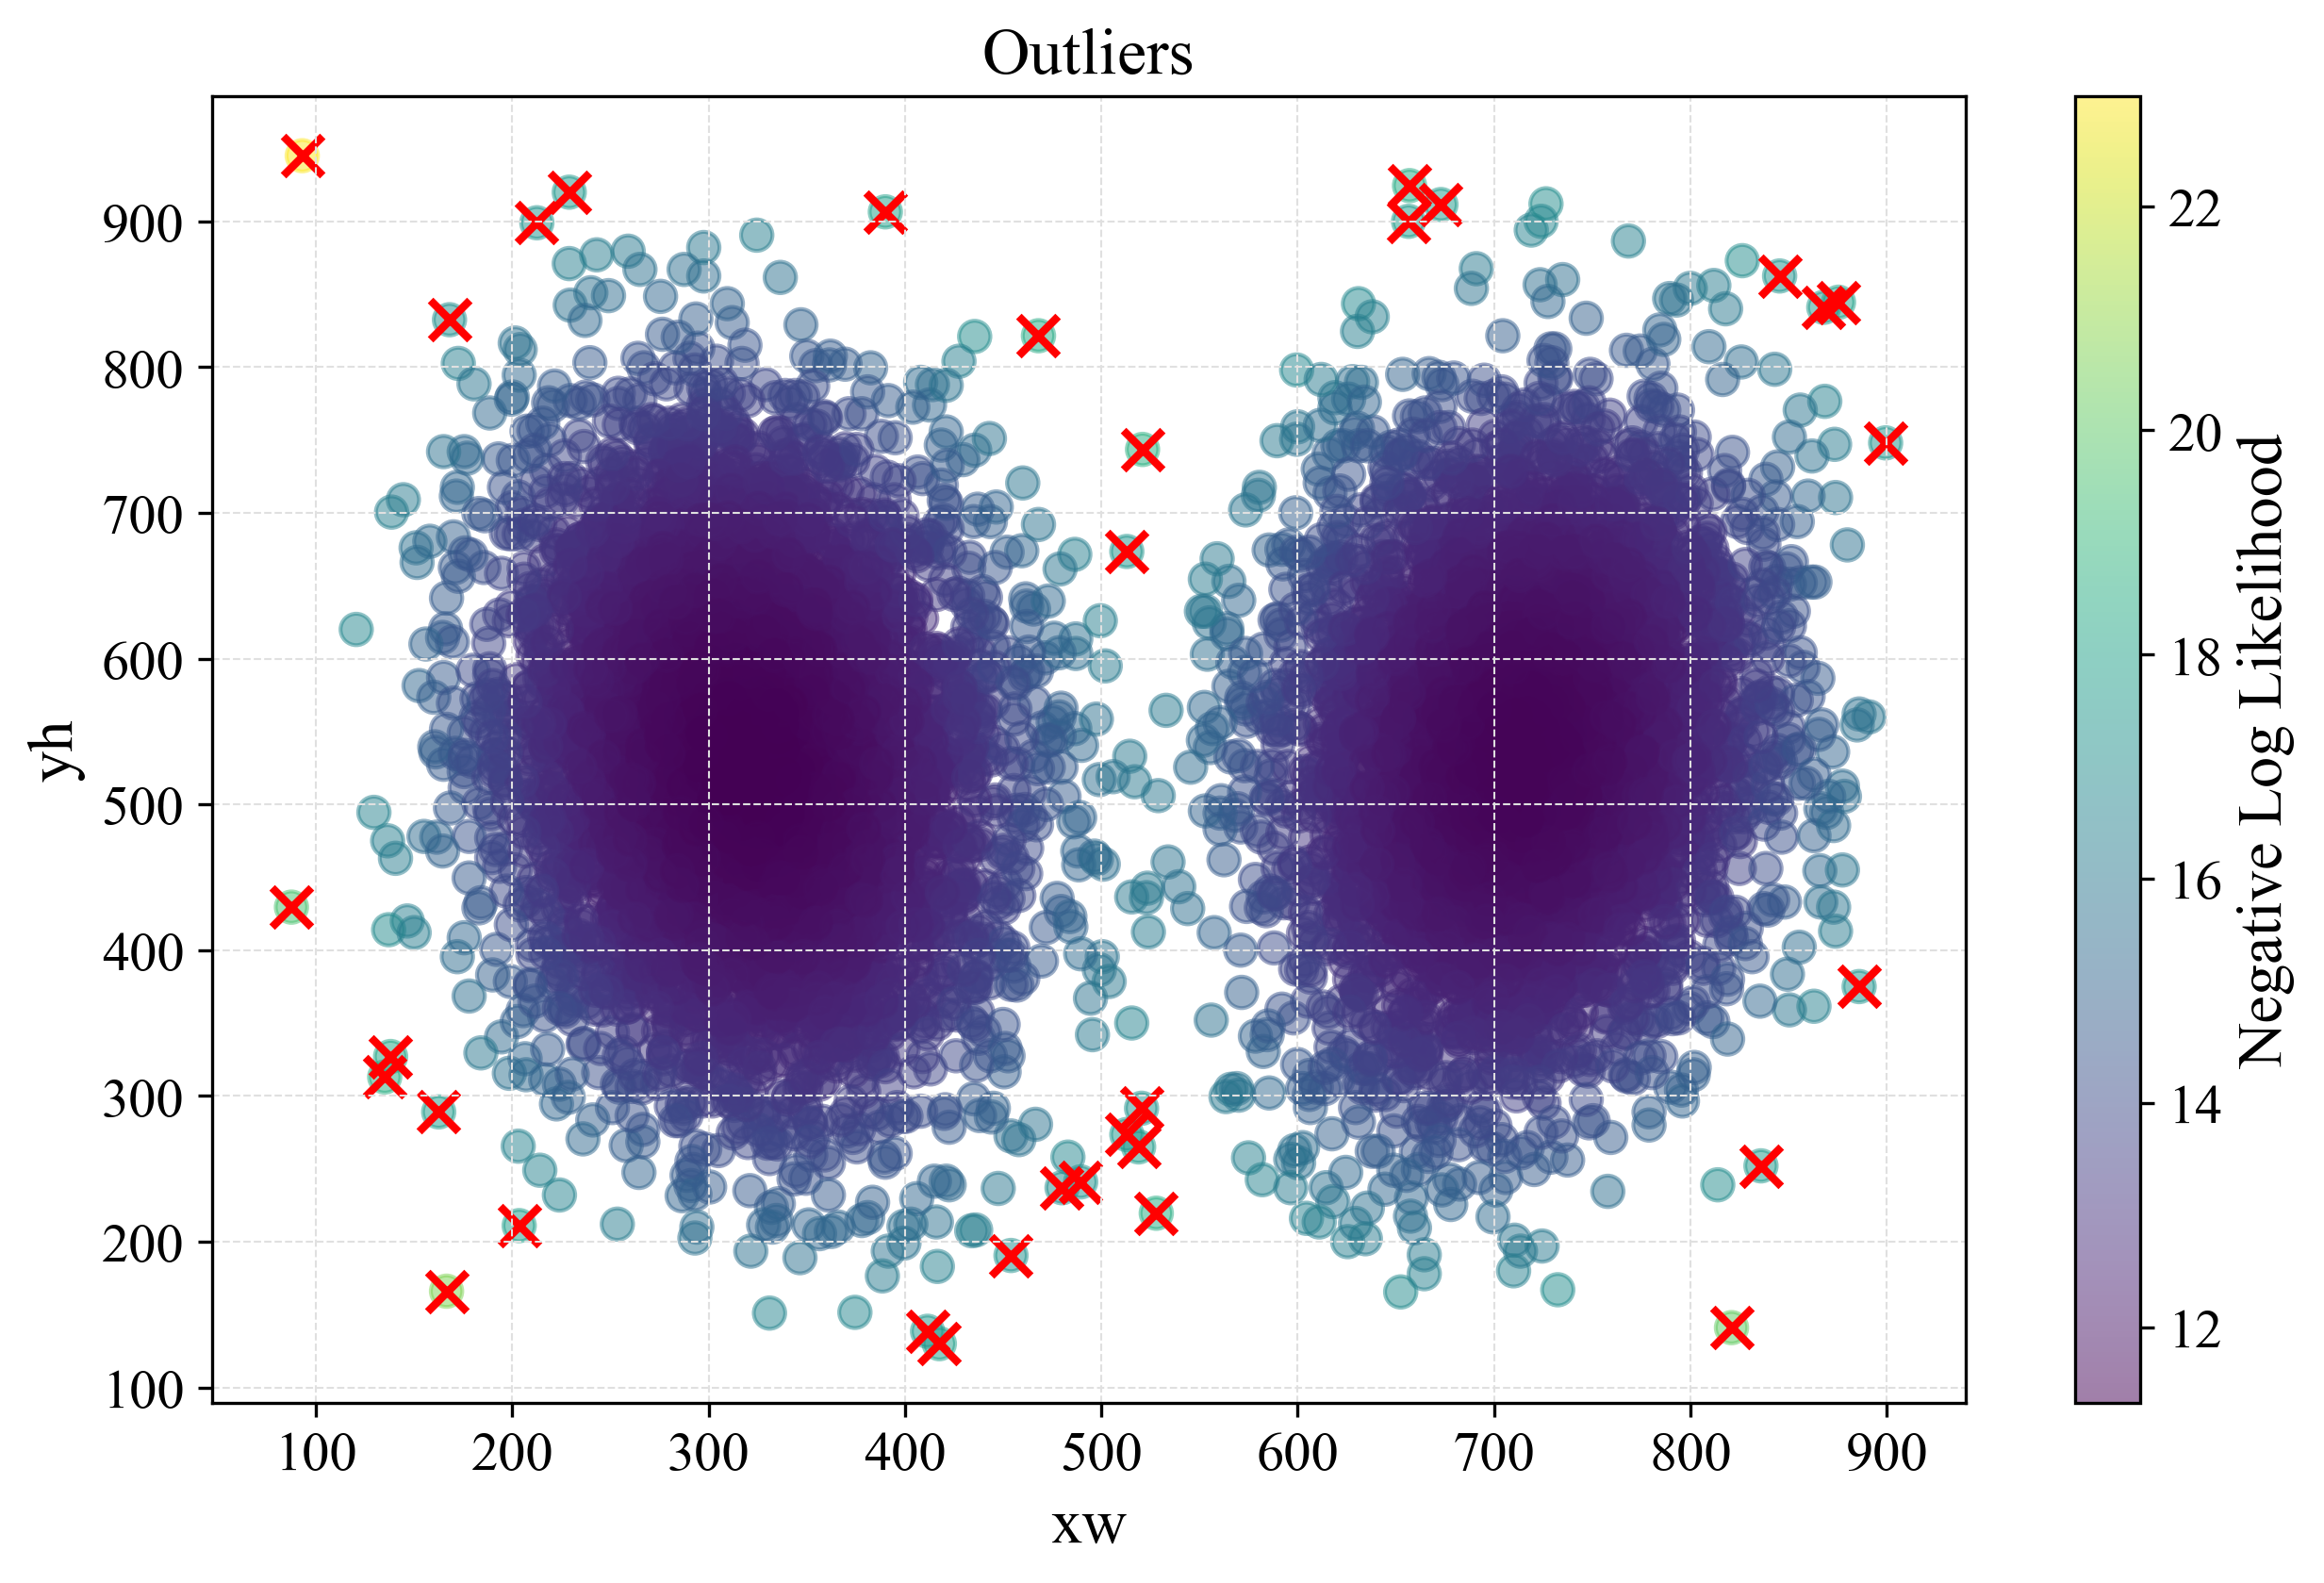
\includegraphics[width = 0.8\textwidth]{figures/Figure20.png}
        \caption{Scatter plot of bounding box centers before outlier removal}
        \label{fig:cha-2 figure17}
    \end{center}
\end{figure}

\begin{figure}[H]
    \begin{center}
        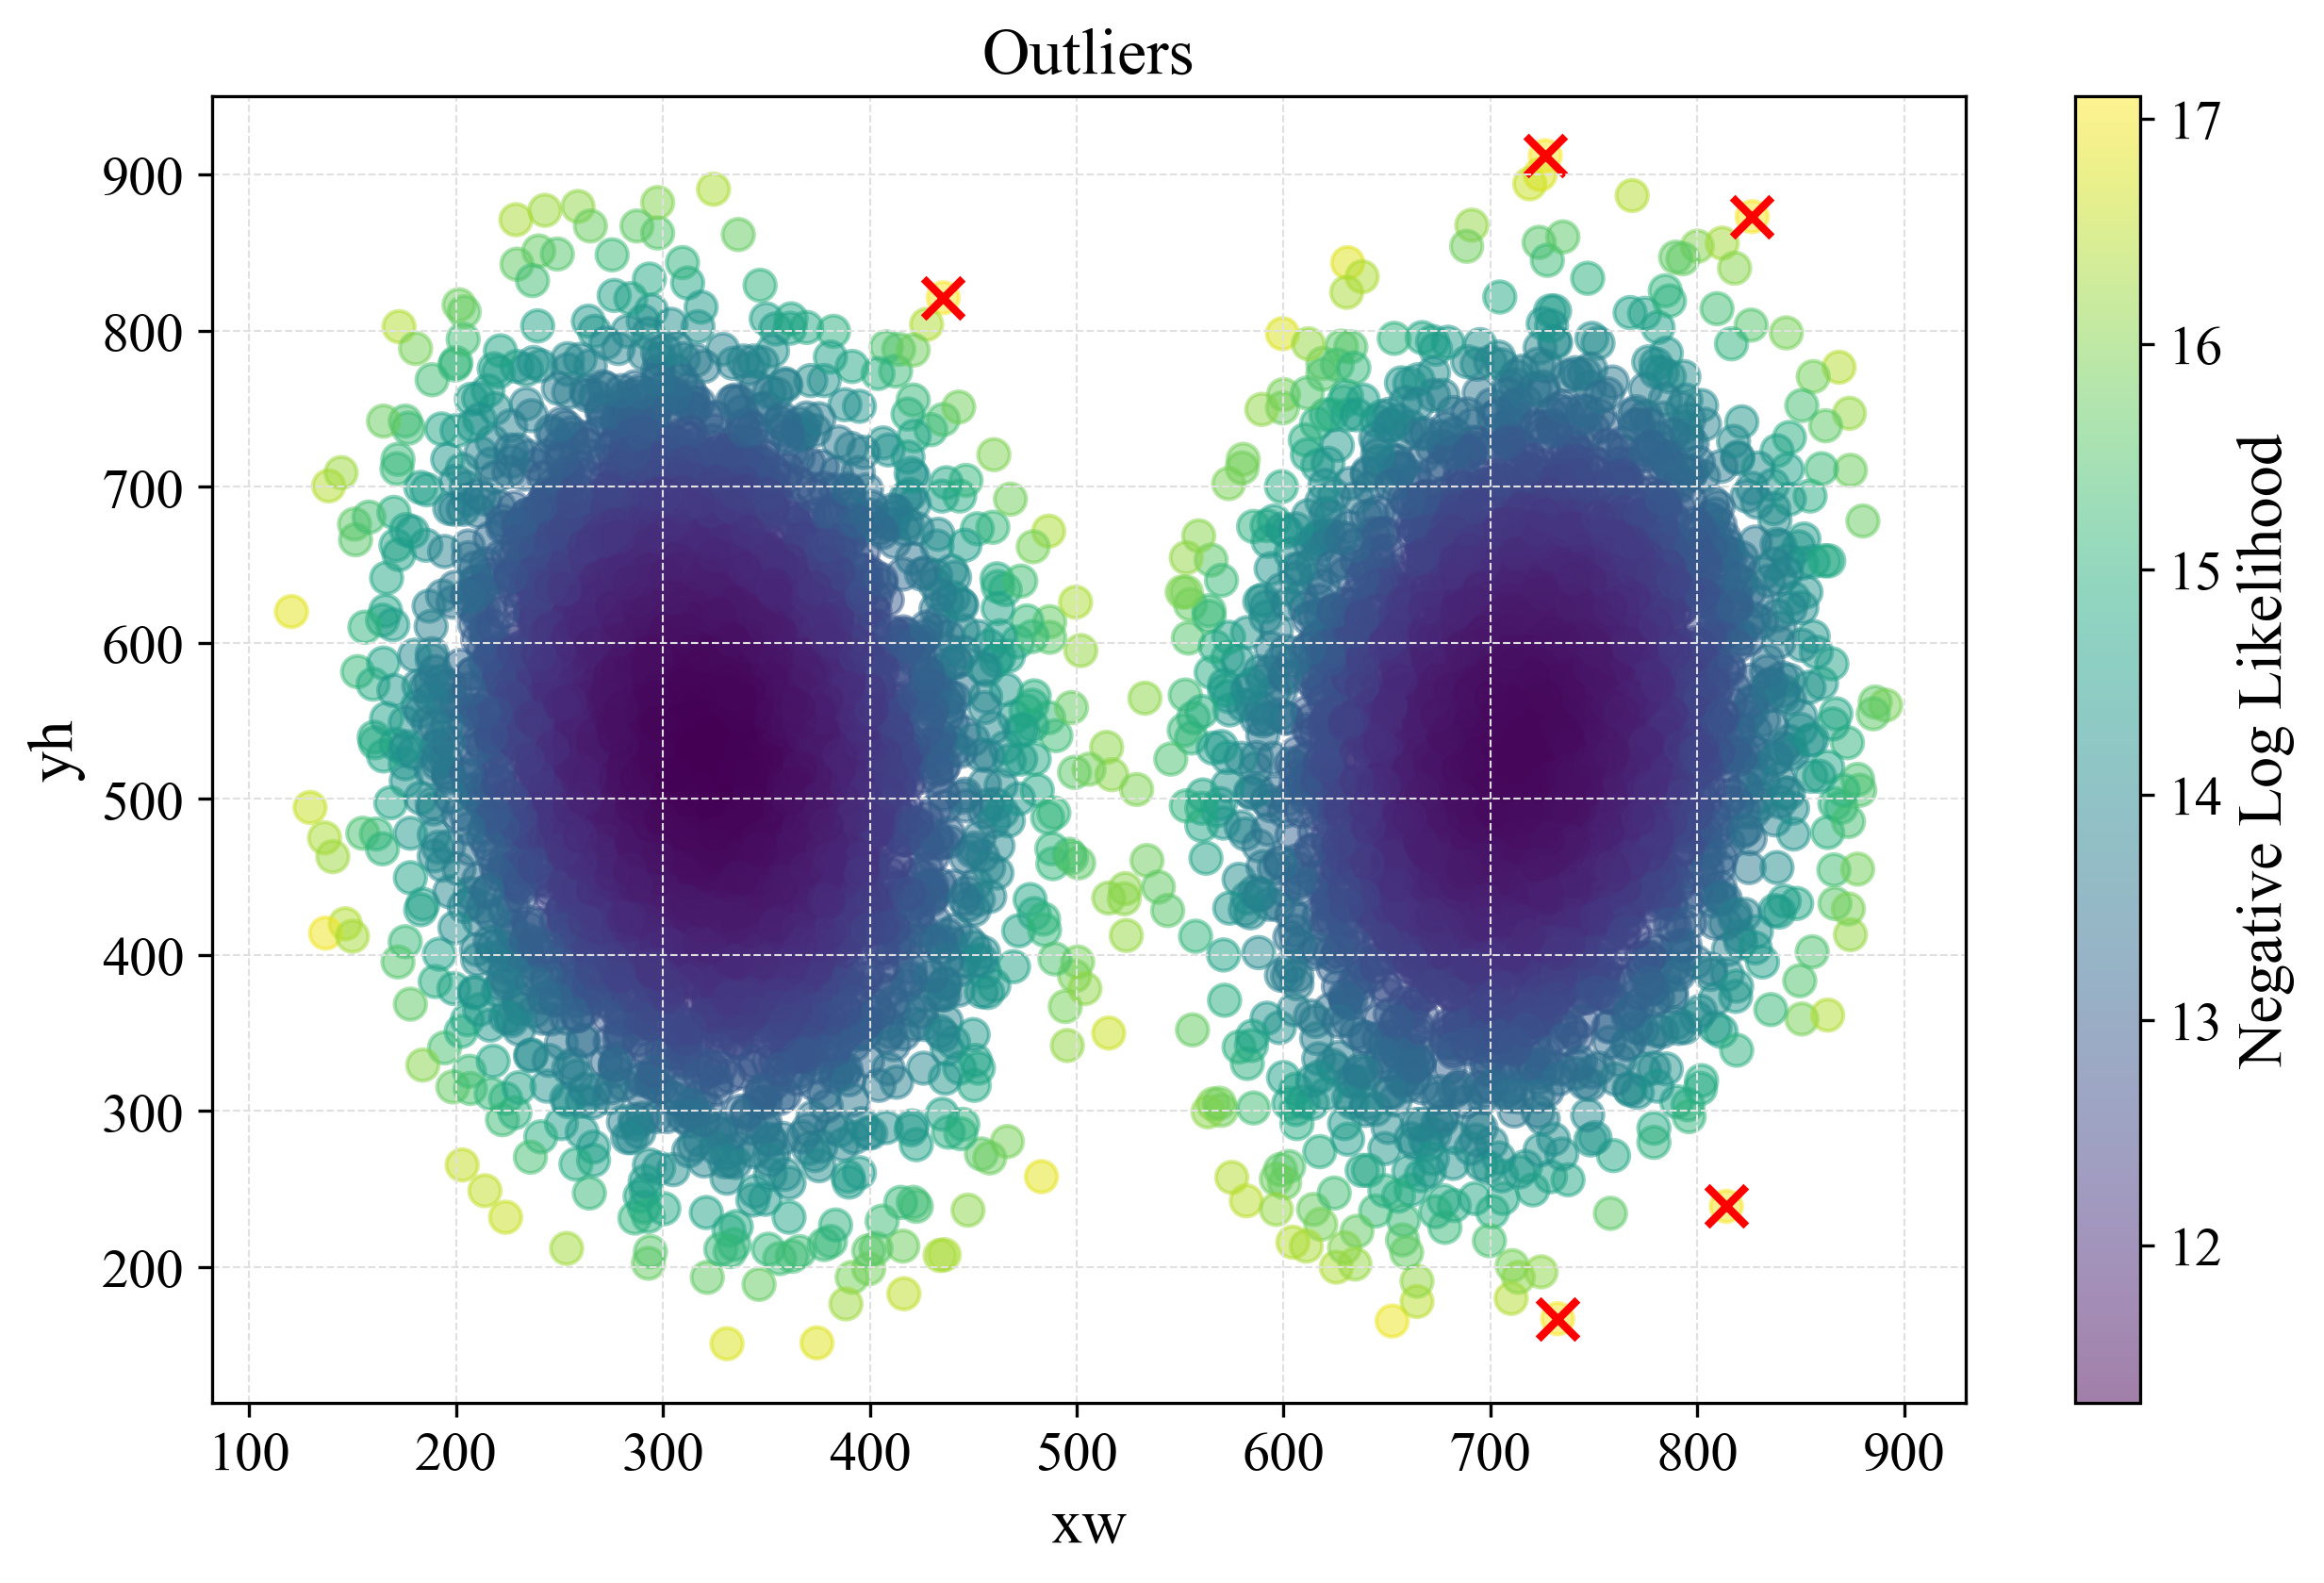
\includegraphics[width = 0.8\textwidth]{figures/Figure21.png}
        \caption{Scatter plot of bounding box centers after initial outlier removal}
        \label{fig:cha-2 figure18}
    \end{center}
\end{figure}

\begin{figure}[H]
    \begin{center}
        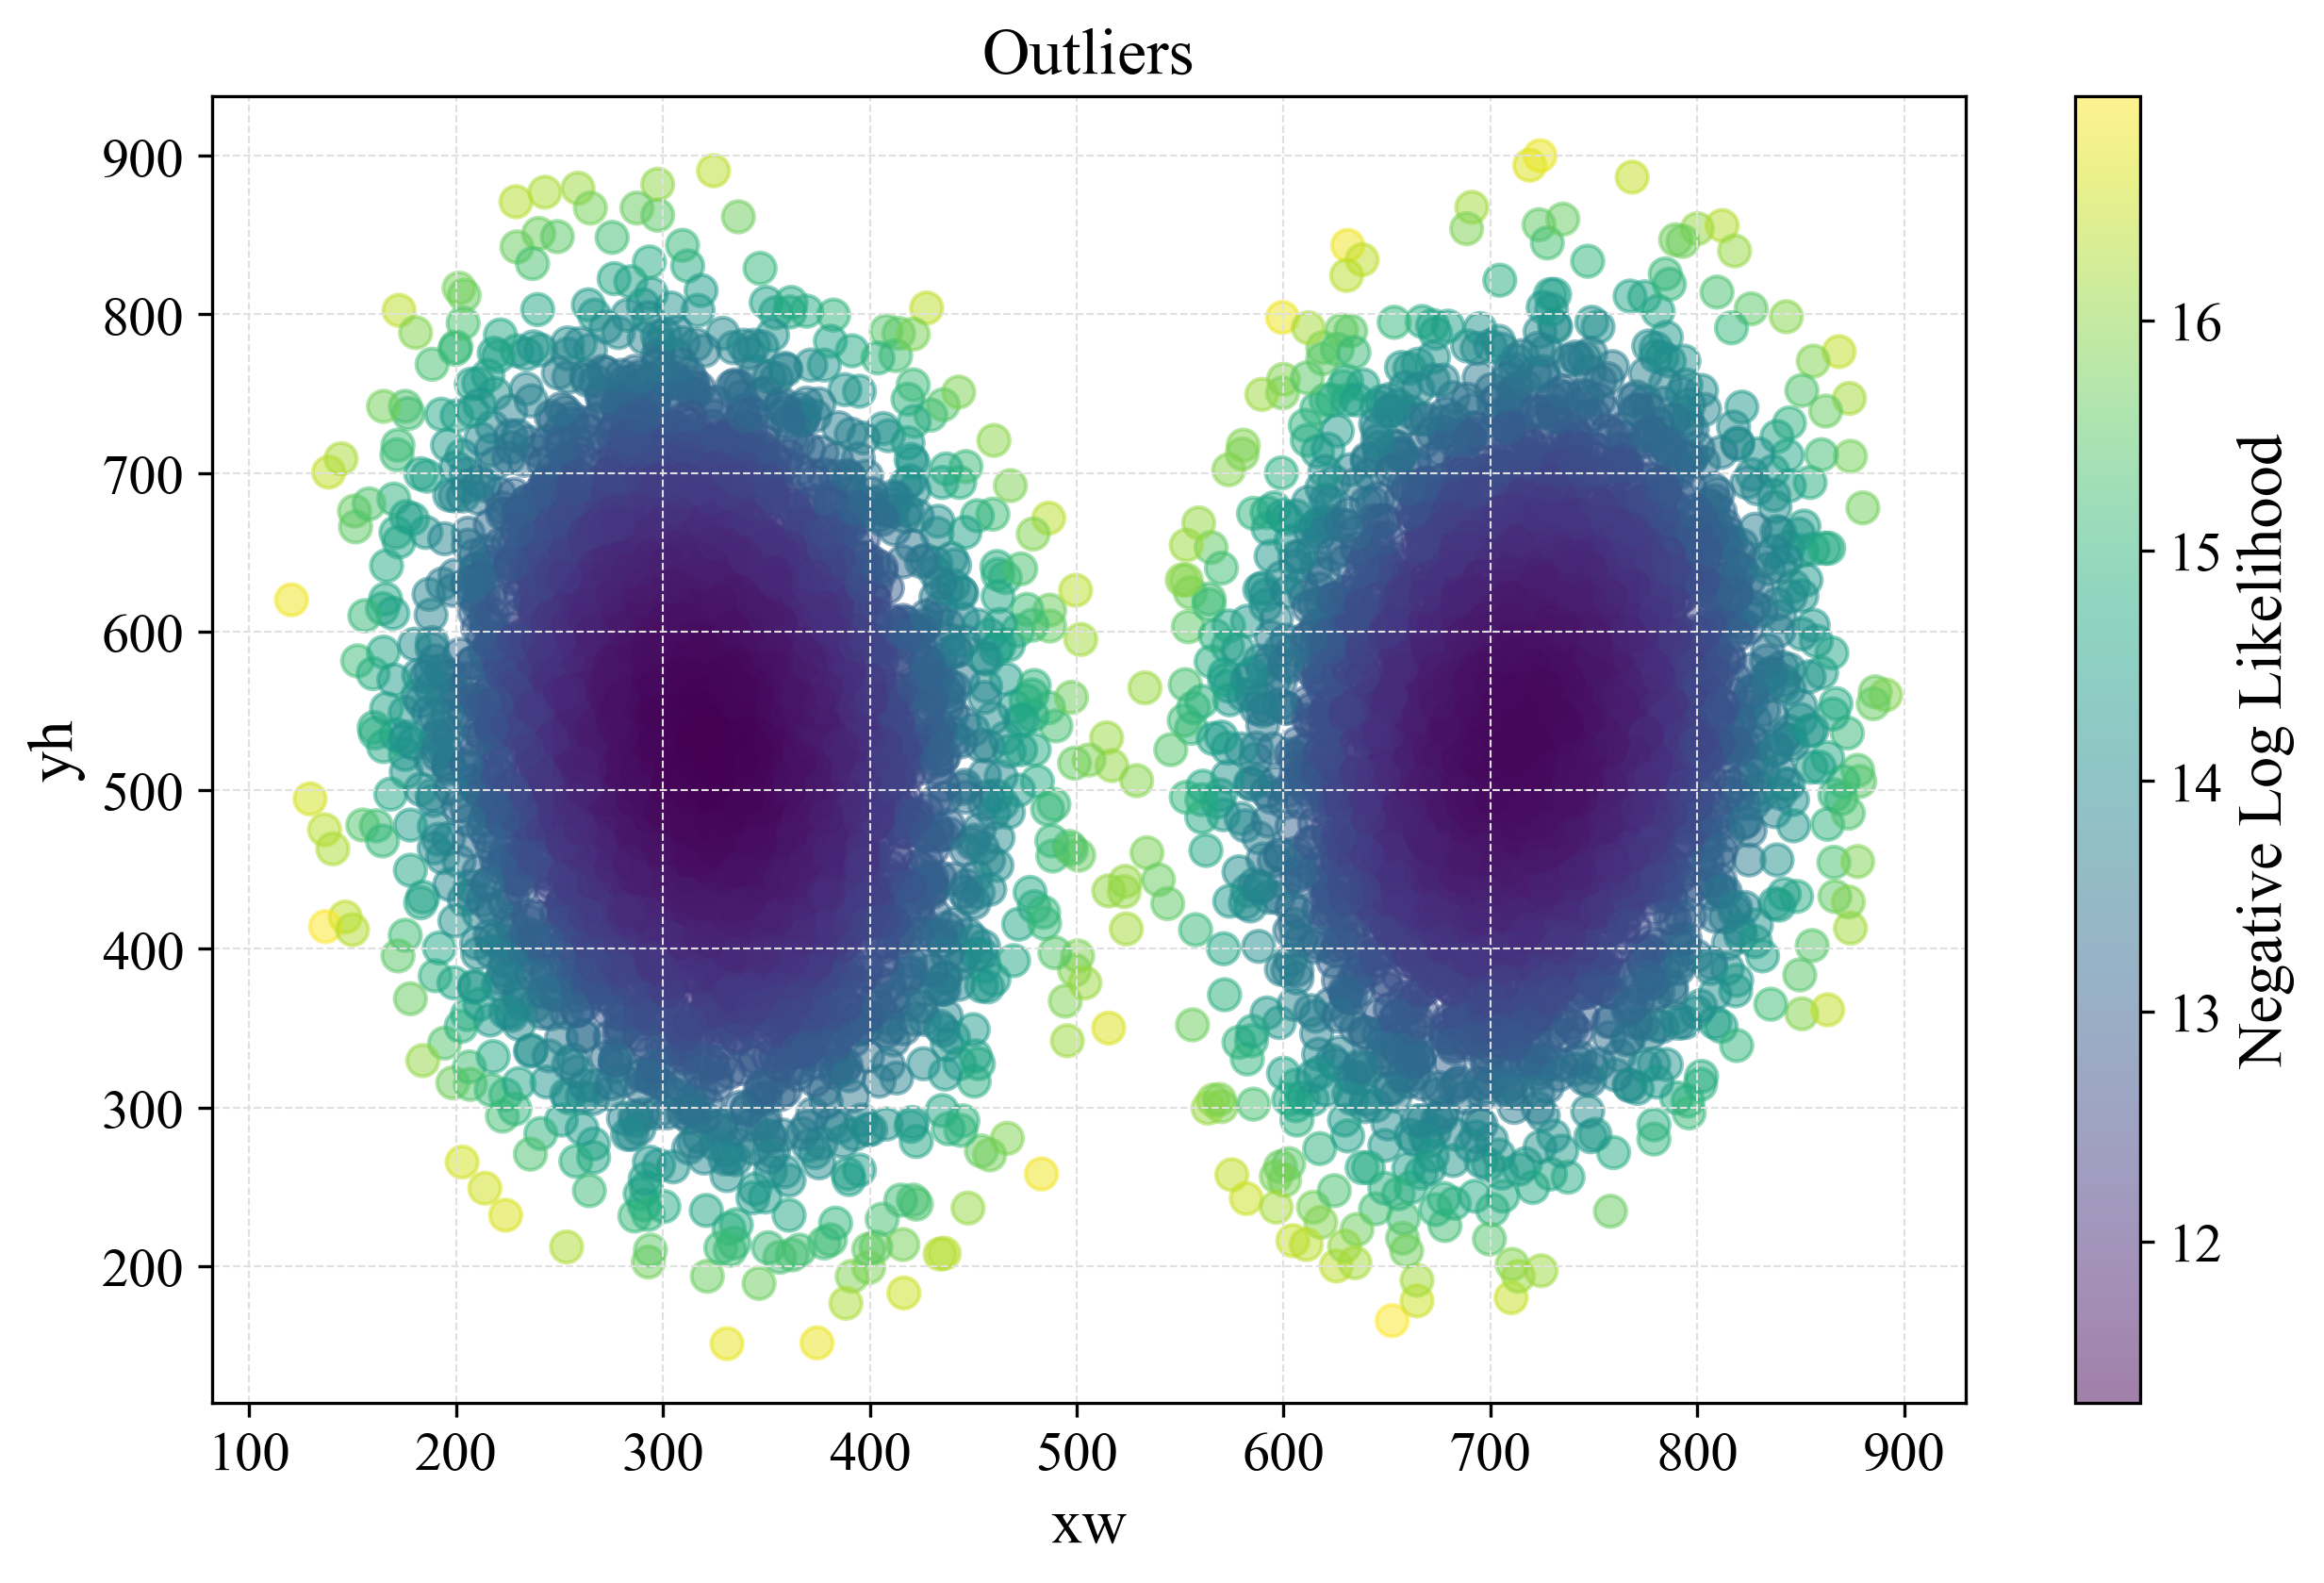
\includegraphics[width = 0.8\textwidth]{figures/Figure22.png}
        \caption{Scatter plot of bounding box centers after final outlier removal}
        \label{fig:cha-2 figure19}
    \end{center}
\end{figure}

The heatmap provides a density representation of the bounding box centers. The color intensity indicates the negative log-likelihood, with higher values representing lower likelihoods (potential outliers). Outliers are indicated by lower density areas (lighter colors), as they are less likely to belong to the main Gaussian components.

\subsection{Visualization of Images}
\label{subsec:chap2 section 1.6}

Visualizing the chest radiographs is a crucial step in understanding the dataset and the differences between normal, abnormal (no lung opacity), and pneumonia (lung opacity) cases. This section presents examples of images from each class with and without bounding boxes.

Figure ~\ref{fig:cha-2 figure20} shows samples of chest radiographs with \emph{Normal} class labels. The images are displayed without any bounding boxes, as these cases do not have pneumonia or lung opacities.

\begin{figure}[H]
    \begin{center}
        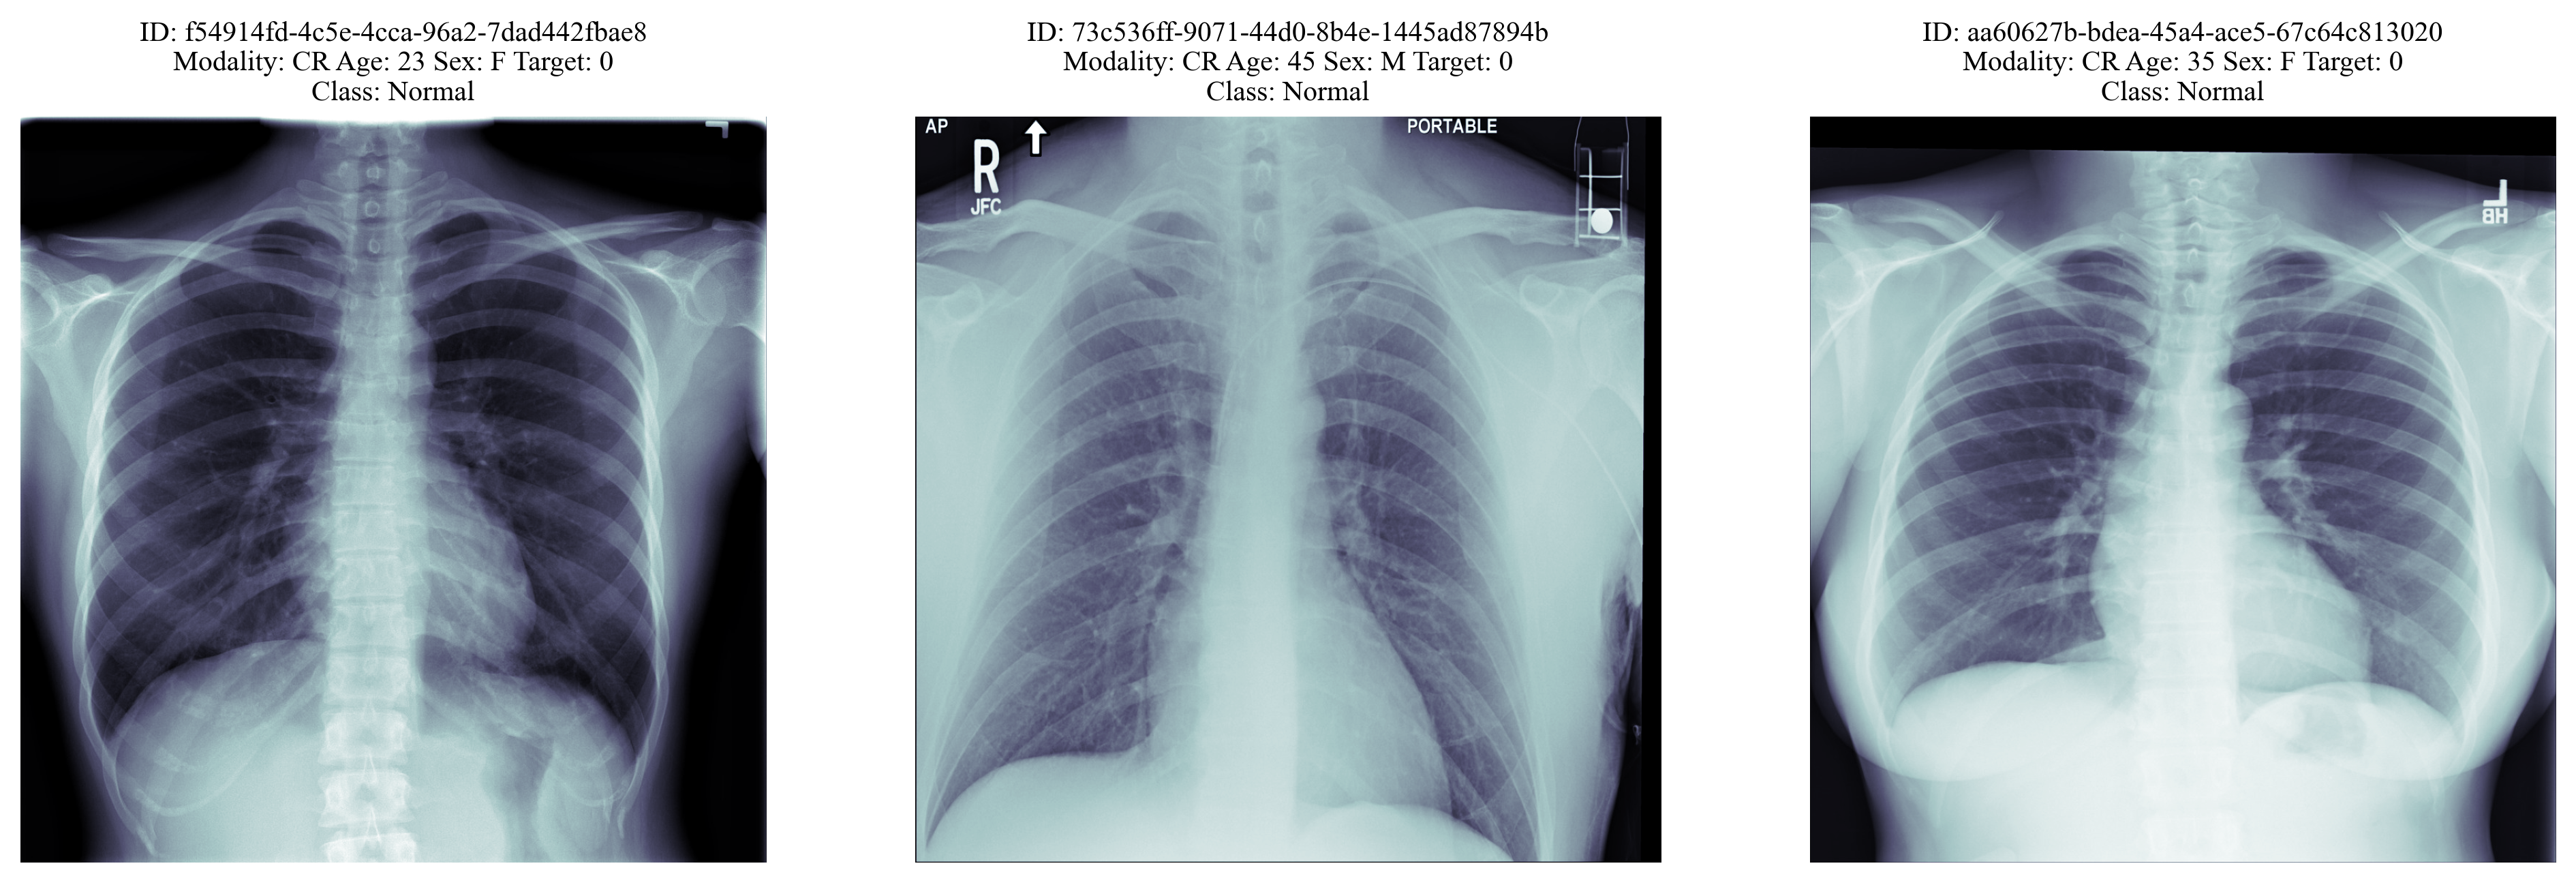
\includegraphics[width = \textwidth]{figures/Figure24.png}
        \caption{Sample images with Normal class labels}
        \label{fig:cha-2 figure20}
    \end{center}
\end{figure}

Figure ~\ref{fig:cha-2 figure21} shows samples of chest radiographs with \emph{No Lung Opacity / Not Normal} class labels. These images have abnormalities that mimic the appearance of pneumonia but do not have lung opacities. The images are displayed without bounding boxes.

\begin{figure}[H]
    \begin{center}
        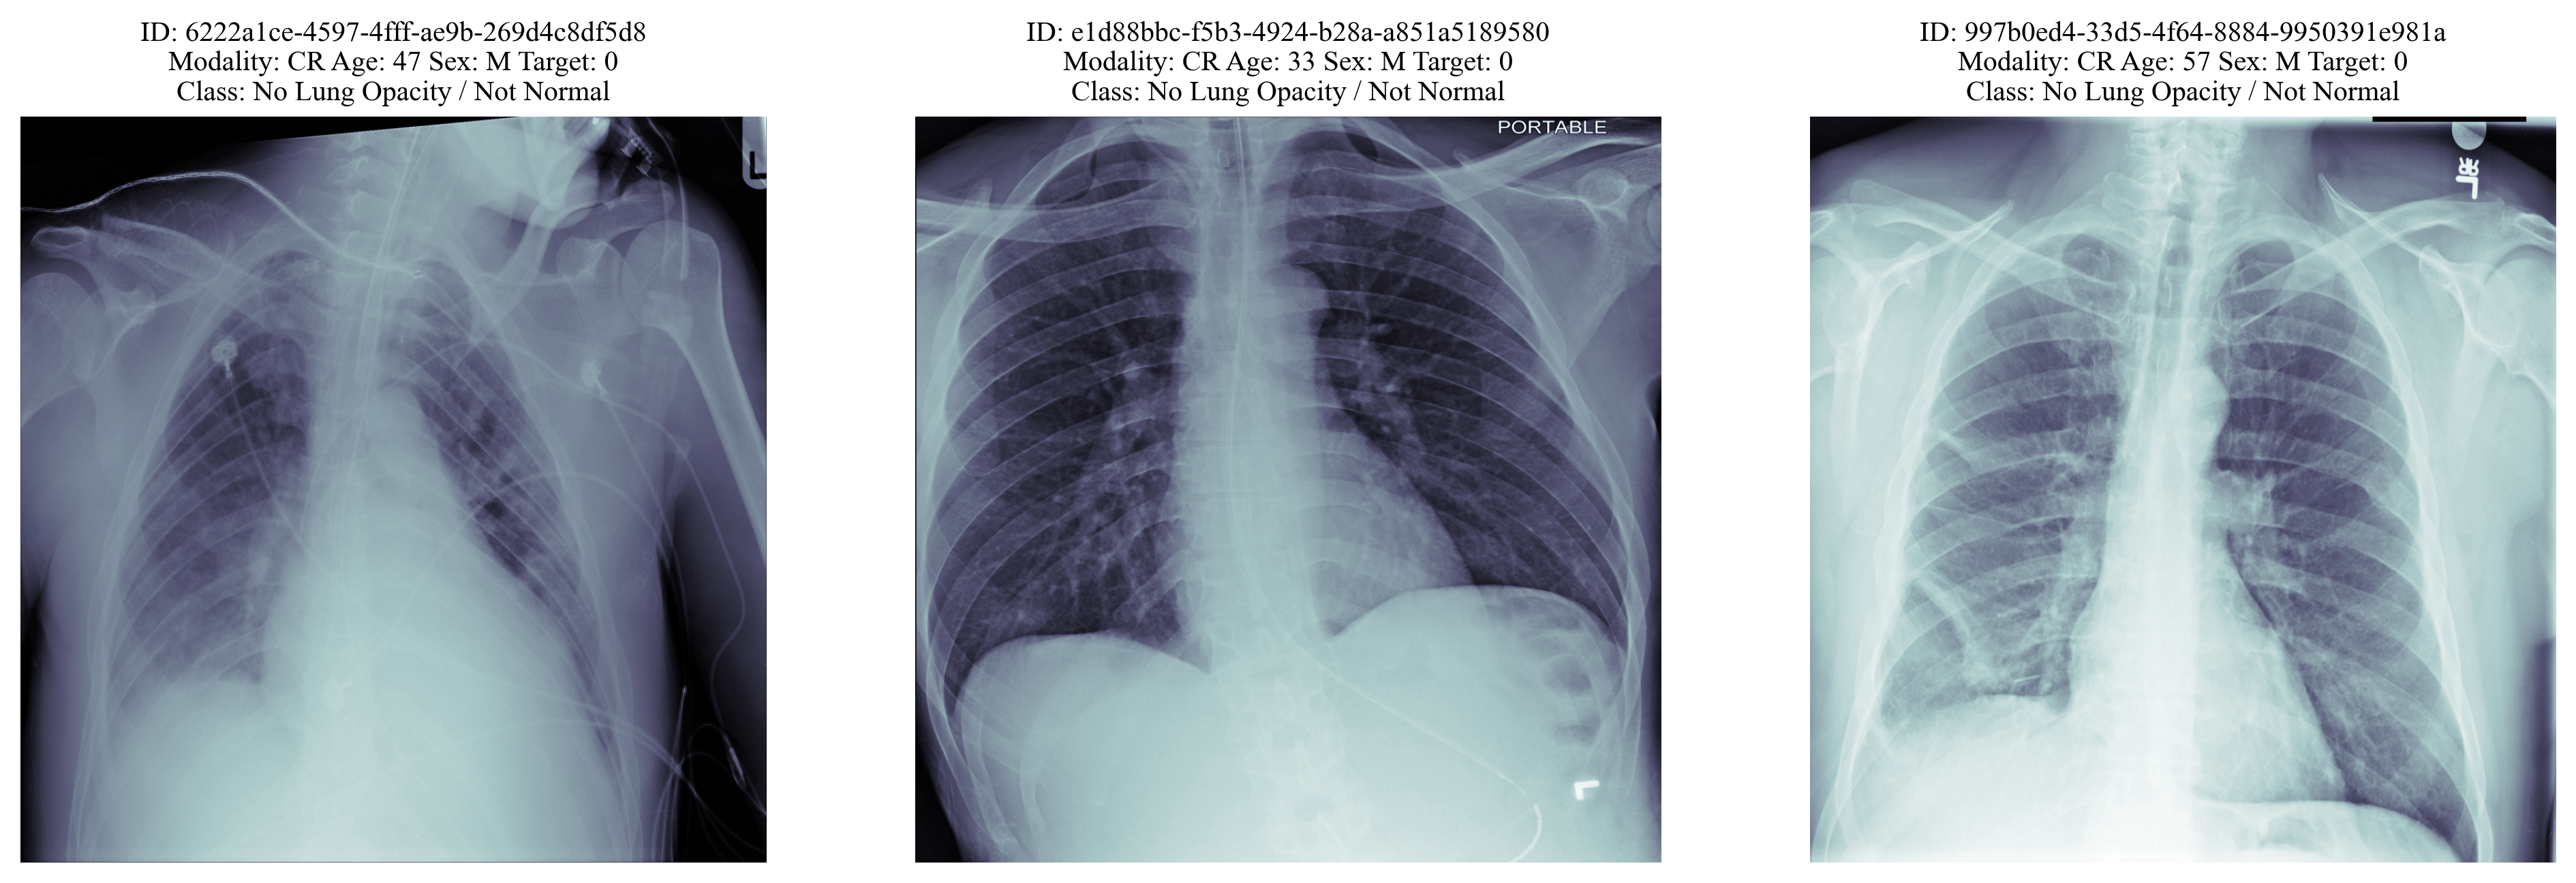
\includegraphics[width = \textwidth]{figures/Figure25.png}
        \caption{Sample images with No Lung Opacity / Not Normal class labels}
        \label{fig:cha-2 figure21}
    \end{center}
\end{figure}

Figure ~\ref{fig:cha-2 figure22} shows samples of chest radiographs with \emph{Lung Opacity} class labels. These images have lung opacities indicative of pneumonia. The images are displayed with bounding boxes that highlight the location of the opacities.

\begin{figure}[H]
    \begin{center}
        
\includegraphics[width = \textwidth]{figures/Figure27.png}
        \caption{Sample images with Lung Opacity class labels}
        \label{fig:cha-2 figure22}
    \end{center}
\end{figure}

\section{Pre-processing}
\label{sec:chap2 section 2}

\subsection{Image Pre-processing}
\label{subsec:chap2 section 2.1}

Pre-processing the image data is a critical step in preparing the dataset for training the deep learning model. The primary goal of pre-processing is to standardize the images, handle missing values or inconsistencies, and ensure that all images are in a suitable format for model training. The code snippet is given in Appendix ~\ref{app:app-A section1}.

This function performs the following key tasks:
\begin{enumerate}
    \item Reading DICOM Images: It iterates over each row in the dataset, reading the DICOM images using the \emph{dcmread} function from the \emph{pydicom} library.
    \item Standardizing Image Channels: It checks the shape of each image and converts it to a 3-channel format if it is not already in this format. This is crucial because DICOM images do not have color channels, and ensuring a consistent shape is important for model training.
    \item Normalization: The pixel values of the images are normalized to a range between 0 and 255. This step enhances the contrast and makes the images more suitable for deep learning.
    \item Resizing Images: Each image is resized to a standard size using OpenCV's \emph{cv2.resize} function. This ensures that all images have the same dimensions, which is a requirement for input to convolutional neural networks (CNNs).
    \item Data Storage: The patient IDs, labels, images, and targets are stored in separate lists and returned as NumPy arrays. These arrays are used as inputs for the deep learning model.
\end{enumerate}

A processed image is depicted in Figure ~\ref{fig:cha-2 figure23}.

\begin{figure}[H]
    \begin{center}
        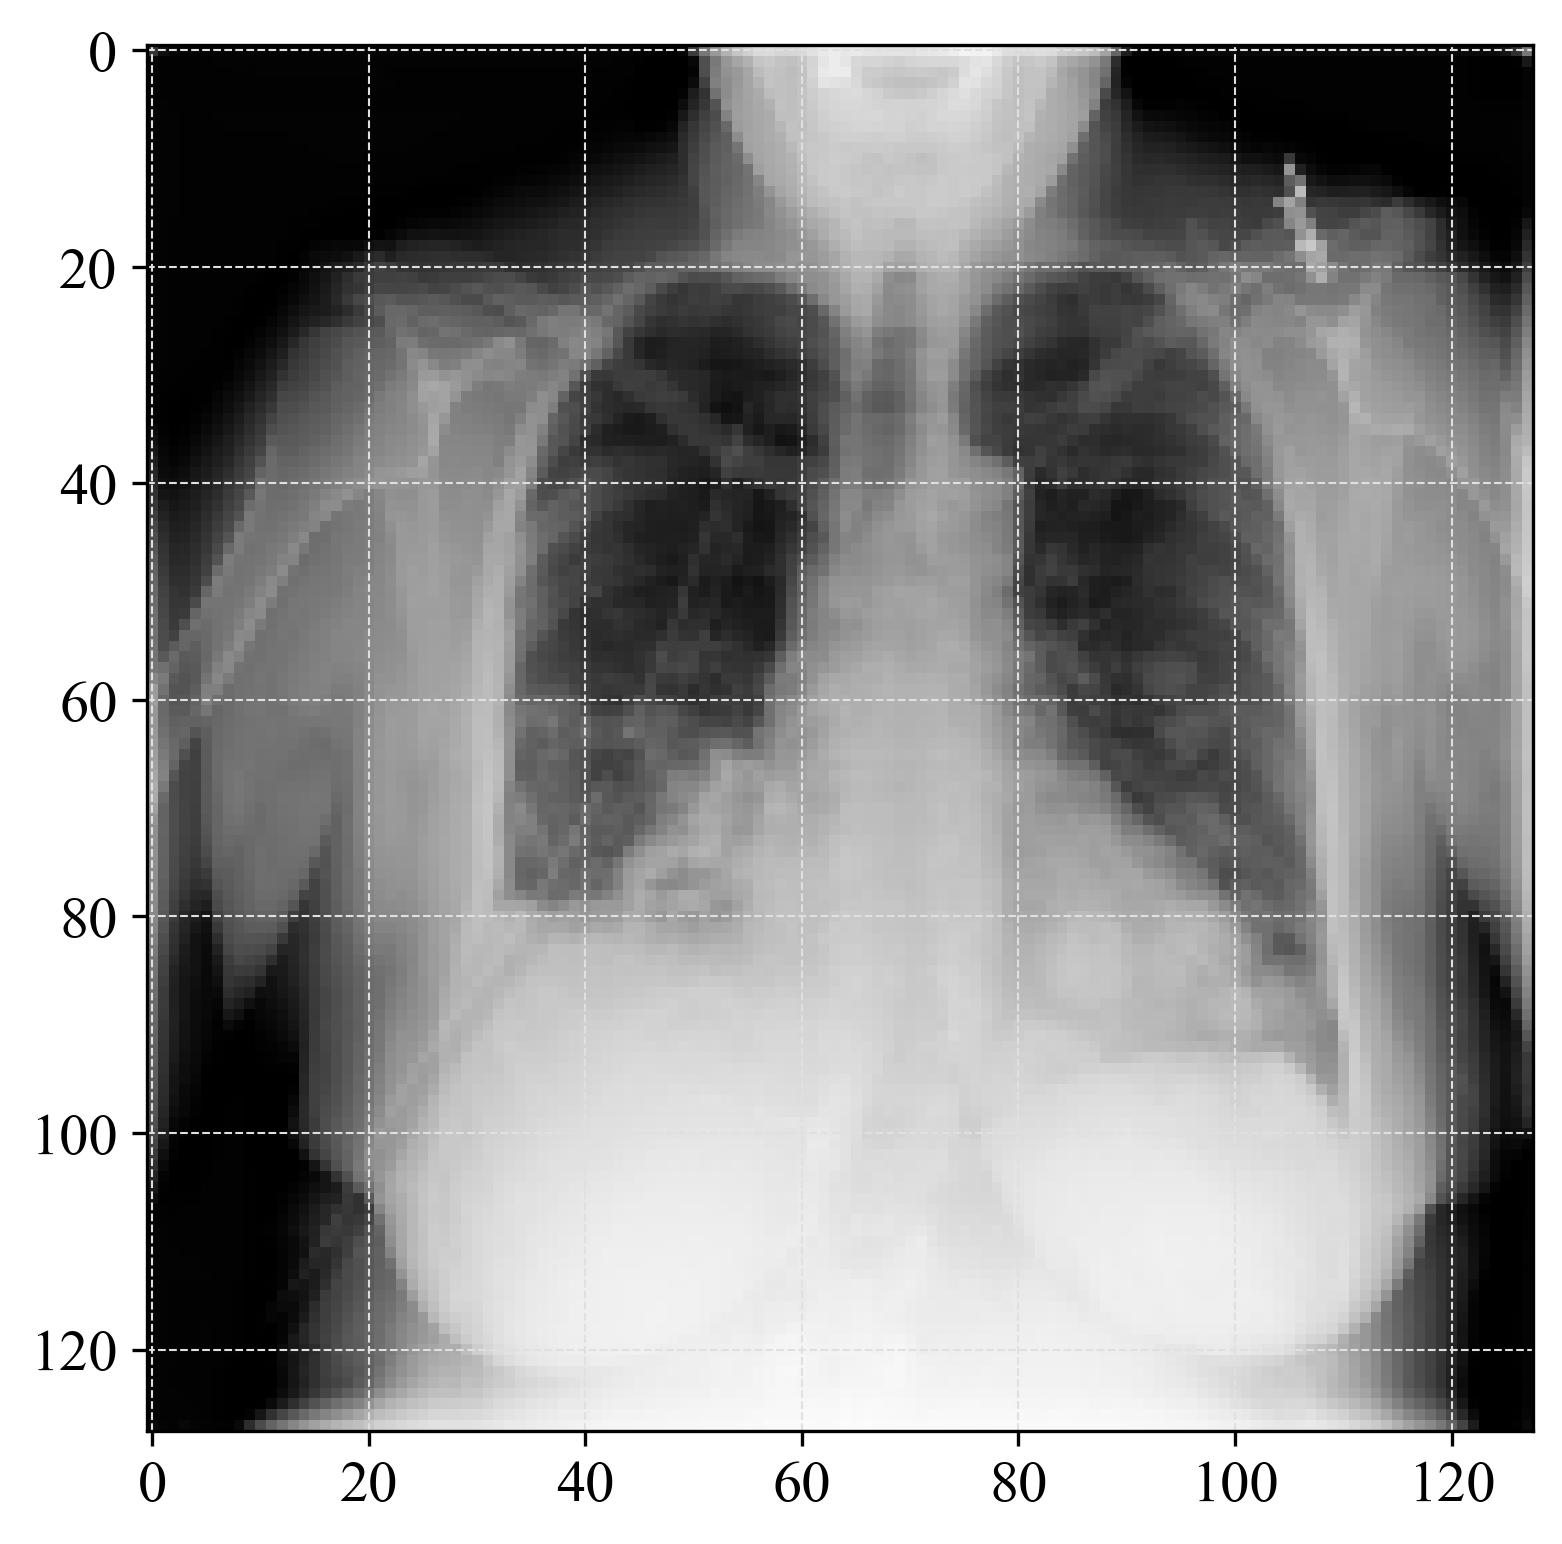
\includegraphics[width = 0.6\textwidth]{figures/Figure28.png}
        \caption{Processed Image after Pre-processing}
        \label{fig:cha-2 figure23}
    \end{center}
\end{figure}

\subsection{Splitting the Dataset}
\label{subsec:chap2 section 2.2}

After pre-processing the image data, the next crucial step is to split the dataset into training and evaluation sets. This allows us to train the deep learning model on one subset of the data while using another subset to evaluate its performance. An 80:20 split was chosen for this task, meaning 80\% of the data is used for training the model, and 20\% is used for evaluation.

The data splitting process was implemented using the \emph{train\_test\_split} function from the \\ \emph{sklearn.model\_selection} module. The function shuffles the data and splits it into training and evaluation sets based on the specified ratio.
\section{Insights and Observations}
\label{sec:chap2 section 3}

\subsection{Summary of EDA Findings}
\label{subsec:chap2 section 3.1}

The exploratory data analysis (EDA) of the chest radiographs dataset provided crucial insights into the data's characteristics, essential for effective model training and evaluation. The dataset comprises images in DICOM format, including metadata such as patient ID, age, sex, and class labels indicating the presence or absence of pneumonia. The class distribution is moderately balanced, with 39\% of the data labeled as "No Lung Opacity / Not Normal", 32\% as "Lung Opacity", and 29\% as "Normal". The age distribution is roughly normal across all classes, peaking around the age of 50 to 60 years. Both male and female patients are included, with a slight predominance of male patients in the "Lung Opacity" class. The dataset contains two primary view positions, PA and AP, evenly distributed. Bounding boxes provided for the "Lung Opacity" class indicate regions of pneumonia, with their centers analyzed to understand typical locations within the radiographs. Initial outliers based on patient age and further outliers based on bounding box centers were detected and handled to ensure data quality. Image pre-processing involved converting images to a consistent 3-channel format, normalizing them, and resizing to a standard size for model training.

\subsection{Impact on Model Development}
\label{subsec:chap2 section 3.2}

The EDA findings significantly influenced the model development process, guiding essential pre-processing steps and data splitting strategies. Understanding the class distributions and patient demographics helped in creating a balanced and representative training dataset, preventing model bias. The analysis of bounding boxes and handling of outliers ensured that the model focused on accurate regions within the radiographs, enhancing its detection capabilities. The decision to split the dataset into training and evaluation sets with an 80:20 ratio provided a robust framework for assessing the model's performance on unseen data, mitigating overfitting. Visualizations of class differences and bounding box locations offered valuable insights into the dataset's complexity, informing the model's architecture and training parameters. By addressing these factors during EDA, we ensured that the deep learning model for pneumonia detection is both well-trained and capable of generalizing effectively to new data, ultimately improving its accuracy and reliability in clinical settings.
